% KLTN template (HCMUS) adapted for the HSGE thesis — English report.
% Build order: clean aux files, then PDFLATEX > BIBTEX > PDFLATEX > PDFLATEX.
%   rm -f *.aux *.bbl *.blg *.log *.out *.toc *.lof *.lot *.run.xml *-blx.bib
%   rm -f Chapter*/*.aux Appendix/*.aux
%   pdflatex -interaction=nonstopmode main.tex && bibtex main
%   pdflatex -interaction=nonstopmode main.tex && pdflatex -interaction=nonstopmode main.tex

\documentclass[oneside,a4paper,14pt]{extreport}

% Vietnamese support (needed for the cover page and names)
\usepackage{cmap}
\usepackage[T5]{fontenc}
\usepackage[utf8]{inputenc}
\DeclareTextSymbolDefault{\DH}{T1}

% Times New Roman (URW Nimbus Roman via vntex, T5-compatible) per Faculty rule
\usepackage{mathptmx}

% Bibliography — IEEE style as required by the Faculty guideline
\usepackage[
	style=ieee,
	sorting=nty,
	backend=bibtex,
	defernumbers=true]{biblatex}
\usepackage[unicode,hidelinks]{hyperref}
\addbibresource{References/references.bib}

\makeatletter
\def\blx@maxline{77}
\makeatother
\AtBeginBibliography{\sloppy}

% Figures
\usepackage{graphicx}
\usepackage{float}
\usepackage{amssymb}
\usepackage[nointegrals]{wasysym}
\graphicspath{ {images/} {Figures/} }

% Source code listings (used sparingly)
\usepackage{listings}
\usepackage{color}
\definecolor{codegreen}{rgb}{0,0.6,0}
\definecolor{codegray}{rgb}{0.5,0.5,0.5}
\definecolor{codepurple}{rgb}{0.58,0,0.82}
\definecolor{backcolour}{rgb}{0.95,0.95,0.92}
\lstdefinestyle{mystyle}{
    backgroundcolor=\color{backcolour},
    commentstyle=\color{codegreen},
    keywordstyle=\color{magenta},
    numberstyle=\tiny\color{codegray},
    stringstyle=\color{codepurple},
    basicstyle=\footnotesize,
    breakatwhitespace=false,
    breaklines=true,
    captionpos=b,
    keepspaces=true,
    numbers=left,
    numbersep=5pt,
    showspaces=false,
    showstringspaces=false,
    showtabs=false,
    tabsize=2
}
\lstset{style=mystyle}

% Mathematics and pseudocode
\usepackage{amsmath}
\usepackage{algorithm}
\usepackage[noend]{algpseudocode}
\makeatletter
\def\BState{\State\hskip-\ALG@thistlm}
\renewcommand{\ALG@name}{Thuật toán}
\makeatother
\numberwithin{algorithm}{chapter}
\renewcommand{\algorithmicrequire}{\textbf{Đầu vào:}}
\renewcommand{\algorithmicensure}{\textbf{Đầu ra:}}

% Tables
\usepackage{multirow}
\usepackage{array}
\usepackage{longtable}
\usepackage{booktabs}
\newcolumntype{L}[1]{>{\raggedright\let\newline\\\arraybackslash\hspace{0pt}}m{#1}}
\newcolumntype{C}[1]{>{\centering\let\newline\\\arraybackslash\hspace{0pt}}m{#1}}
\newcolumntype{R}[1]{>{\raggedleft\let\newline\\\arraybackslash\hspace{0pt}}m{#1}}

% 1.5 line spacing (Faculty requirement)
\usepackage{setspace}
\onehalfspacing

% Soften overfull lines caused by unhyphenatable \texttt words
\emergencystretch=1.5em

% Indent first paragraph of each section
\usepackage{indentfirst}

% Number down to subsubsection (Faculty requirement)
\setcounter{secnumdepth}{3}

% Margins per the Faculty formatting guideline:
% top 3cm, bottom 3.5cm, left 3.5cm, right 2cm, page number centered at bottom
\usepackage[
  top=30mm,
  bottom=35mm,
  left=35mm,
  right=20mm,
  includefoot]{geometry}

% Vietnamese names for chapters/figures/tables
\renewcommand{\chaptername}{Chương}
\renewcommand{\figurename}{Hình}
\renewcommand{\tablename}{Bảng}
\renewcommand{\contentsname}{Mục lục}
\renewcommand{\listfigurename}{Danh sách hình}
\renewcommand{\listtablename}{Danh sách bảng}
\renewcommand{\appendixname}{Phụ lục}

% Base font size 13pt (Faculty guideline allows 13pt or 14pt).
% NOTE: extreport/extsizes has no 13pt option — passing [13pt] to \documentclass
% silently falls back to 10pt. The fontsize package is the correct way.
\usepackage[fontsize=13pt]{fontsize}

% Tables, figures and captions are set single-spaced (body text stays at 1.5).
\usepackage{etoolbox}
\AtBeginEnvironment{table}{\singlespacing}
\AtBeginEnvironment{longtable}{\singlespacing}
\AtBeginEnvironment{figure}{\singlespacing}
\AtBeginEnvironment{algorithm}{\singlespacing}

% Cover page
\usepackage{tikz}
\usetikzlibrary{calc, positioning, arrows.meta, shapes.geometric}
\newcommand\HRule{\rule{\textwidth}{1pt}}

% ======================================================================== %
% Thesis metadata — filled once here, reused everywhere                    %
% ======================================================================== %
\newcommand{\tenSV}{Trương~Bảo~Kiệt~--~22127223~--~Hồ~Tiến~Phát~--~22127321}
\newcommand{\mssv}{22127223~--~22127321}
\newcommand{\tenKL}{Data~Construction~and~Fine-tuning~of~Small~Language~Models~for~Web~AI~Agents}
\newcommand{\tenGVHD}{Assoc.~Prof.~Dr.~Nguyễn~Văn~Vũ}
\newcommand{\tenBM}{Software Engineering}

\begin{document}

% !TEX root = ../main.tex
\newcommand{\titlepageframe}{%
\begin{tikzpicture}[remember picture, overlay]
  \draw[line width=2pt]
    ($(current page.north west) + (2cm,-2cm)$)
    rectangle
    ($(current page.south east) + (-1.5cm,2cm)$);
\end{tikzpicture}}

\begin{titlepage}
\titlepageframe

\begin{center}
{\bfseries TRƯỜNG ĐẠI HỌC KHOA HỌC TỰ NHIÊN\\
KHOA CÔNG NGHỆ THÔNG TIN}\\[2.5cm]

{\bfseries TRƯƠNG BẢO KIỆT - HỒ TIẾN PHÁT}\\[2.5cm]

{\large \bfseries \setlength{\baselineskip}{22pt}
XÂY DỰNG DỮ LIỆU VÀ TINH CHỈNH \\
MÔ HÌNH NGÔN NGỮ NHỎ \\
CHO TÁC NHÂN TRÍ TUỆ NHÂN TẠO TRÊN WEB}\\[4.5cm]

{\bfseries KHÓA LUẬN TỐT NGHIỆP CỬ NHÂN CNTT\\
CHƯƠNG TRÌNH CHẤT LƯỢNG CAO}\\[2.5cm]

\vspace*{\fill}
{\bfseries TP. HỒ CHÍ MINH, THÁNG 08/2026}\\[0.5cm]

\end{center}

\end{titlepage}

\begin{titlepage}
\titlepageframe

\begin{center}

{\bfseries TRƯỜNG ĐẠI HỌC KHOA HỌC TỰ NHIÊN\\
KHOA CÔNG NGHỆ THÔNG TIN}\\[2.5cm]

{\bfseries TRƯƠNG BẢO KIỆT - 22127223\\
HỒ TIẾN PHÁT - 22127321}\\[2.5cm]

{\large \bfseries \setlength{\baselineskip}{22pt}
XÂY DỰNG DỮ LIỆU VÀ TINH CHỈNH \\
MÔ HÌNH NGÔN NGỮ NHỎ \\
CHO TÁC NHÂN TRÍ TUỆ NHÂN TẠO TRÊN WEB}\\[2cm]

{\bfseries KHÓA LUẬN TỐT NGHIỆP CỬ NHÂN CNTT\\
CHƯƠNG TRÌNH CHẤT LƯỢNG CAO}\\[2cm]

{\bfseries GIÁO VIÊN HƯỚNG DẪN}\\
{\bfseries PGS.TS. NGUYỄN VĂN VŨ}\\[1.5cm]

\vspace*{\fill}
{\bfseries TP. HỒ CHÍ MINH, THÁNG 08/2026}\\[0.5cm]

\end{center}

\end{titlepage}

% After the title pages, the advisor's and reviewer's evaluation sheets are
% inserted here when binding the final copy (provided after the defense).

\pagenumbering{roman}

\addcontentsline{toc}{chapter}{Lời cảm ơn}
\chapter*{Lời cảm ơn}

% TODO: cá nhân hóa trước khi nộp.
Chúng em xin gửi lời cảm ơn chân thành đến thầy hướng dẫn, PGS.TS. Nguyễn
Văn Vũ, vì sự tận tình chỉ bảo, kiên nhẫn và những góp ý quý báu trong suốt
quá trình thực hiện khóa luận. Chúng em cũng xin cảm ơn quý thầy cô Khoa
Công nghệ Thông tin, Trường Đại học Khoa học Tự nhiên, ĐHQG-HCM, đã truyền
đạt kiến thức và hỗ trợ chúng em trong những năm học vừa qua.

Cuối cùng, chúng em xin cảm ơn gia đình và bạn bè đã luôn động viên trong
suốt thời gian thực hiện đề tài.

\begin{flushright}
Tp. Hồ Chí Minh, tháng 08 năm 2026\\
\textit{Nhóm sinh viên thực hiện}\\
Trương Bảo Kiệt -- Hồ Tiến Phát
\end{flushright}


% Đề cương chi tiết — bắt buộc theo checklist của Khoa, đặt ngay sau Lời cảm
% ơn và trước Mục lục. Bản nộp SAU bảo vệ phải thay bằng bản scan có chữ ký.
% Số liệu trong Appendix/decuongchitiet.tex là hiện trạng tại thời điểm nộp đề
% cương (370 mẫu, GitLab 10/180 vs 12/180); §2.3.3 của file đó nói rõ điều này
% và trỏ sang Chương 4 cho kết quả cuối, nên hai bản không mâu thuẫn nhau.
% TẠM BỎ khỏi bản build (yêu cầu 19-08) — bỏ dấu %% ở năm dòng dưới để bật lại.
% Bắt buộc bật trước khi nộp: checklist nộp cuốn báo cáo của Khoa có mục "Đề
% cương chi tiết". Quy định cũng ghi rõ đề cương KHÔNG được đánh số trang, và
% số La Mã tiếp tục từ Mục lục — nên khối này tắt folio rồi trả bộ đếm trang về
% giá trị cũ, để Lời cảm ơn = i và Mục lục = ii. Không đưa đề cương vào mục lục
% vì nó không có số trang để trỏ tới.
\newcounter{savedfrontpage}
%\setcounter{savedfrontpage}{\value{page}}
%\clearpage\pagestyle{empty}
%% Đề cương chi tiết — bắt buộc theo checklist nộp cuốn báo cáo của Khoa
% (đặt giữa Lời cảm ơn và Mục lục). Bản nộp TRƯỚC bảo vệ không cần chữ ký;
% bản nộp SAU bảo vệ phải có chữ ký GVHD — khi đó thay toàn bộ nội dung
% file này bằng \includepdf bản scan đã ký.

\chapter*{Đề cương chi tiết}
\markboth{Đề cương chi tiết}{Đề cương chi tiết}

\section*{1.\quad THÔNG TIN CHUNG}

\begin{itemize}
  \item \textbf{Tên đề tài:} Xây dựng dữ liệu và tinh chỉnh mô hình ngôn ngữ
  nhỏ cho tác nhân trí tuệ nhân tạo trên web \\
  \textit{(Data Construction and Fine-tuning of Small Language Models for Web
  AI Agents)}
  \item \textbf{Người hướng dẫn:} PGS.TS. Nguyễn Văn Vũ (Khoa Công nghệ
  Thông tin, Trường Đại học Khoa học Tự nhiên, ĐHQG-HCM)
  \item \textbf{Sinh viên thực hiện:}
  \begin{enumerate}
    \item Trương Bảo Kiệt - MSSV 22127223
    \item Hồ Tiến Phát - MSSV 22127321
  \end{enumerate}
  \item \textbf{Loại đề tài:} Nghiên cứu
  \item \textbf{Thời gian thực hiện:} 01/2026 - 08/2026
\end{itemize}

\section*{2.\quad NỘI DUNG THỰC HIỆN}

\subsection*{2.1\quad Giới thiệu về đề tài}

\subsubsection*{2.1.1\quad Bối cảnh và vấn đề}

Trình duyệt là giao diện chung của hầu hết các dịch vụ trực tuyến, nên một
agent phần mềm thao tác được website \emph{qua chính giao diện người dùng} là
một trong những dạng tự động hóa có phạm vi ứng dụng rộng nhất. Các mô hình
ngôn ngữ lớn (LLM) gần đây đã khiến những web agent như vậy trở nên khả thi:
nhận một bản mô tả dạng văn bản của trang cùng một mục tiêu, mô hình quyết
định được cần click hay gõ gì tiếp theo.

Tuy nhiên, năng lực đó hiện gần như chỉ tồn tại ở các mô hình độc quyền rất
lớn truy cập qua API, và sự phụ thuộc này gây tốn kém theo nhiều cách cộng
dồn. Mỗi bước của mỗi task là một lời gọi API trả phí trong khi task của agent
cần rất nhiều bước; độ trễ bị giới hạn bởi dịch vụ từ xa; toàn bộ nội dung mọi
trang được duyệt (có thể chứa dữ liệu riêng tư hoặc nội bộ) bị gửi cho
bên thứ ba; và bản thân mô hình là một hàng hóa cố định mà người vận hành
không kiểm tra hay cải thiện được.

Mô hình ngôn ngữ nhỏ (SLM, cỡ mười tỷ tham số trở xuống, tự triển khai
được trên một GPU) đảo ngược mọi ràng buộc trên. Thứ chúng thiếu là năng
lực. Ngay cả các mô hình lớn cũng thấy task web thực tế là khó: trên benchmark
WebArena gồm các website đầy đủ chức năng tự triển khai, agent dựa trên GPT-4
chỉ hoàn thành khoảng 14\% số task so với khoảng 78\% của con
người~\cite{zhou2024webarena}. Phương thuốc tiêu chuẩn, tinh chỉnh có giám
sát (SFT) trên các bản mẫu hành vi, lại vấp phải bài toán dữ liệu:
trajectory tương tác có gán mục tiêu trên website đích hầu như không tồn tại,
còn thuê người gán nhãn thì đắt, chậm và phải làm lại cho từng website.

Câu hỏi đề tài đặt ra là: liệu có thể xây dựng một pipeline hoàn toàn tự động
\emph{khám phá} một website không nhãn, \emph{tự nghĩ ra} các task có ý nghĩa
dựa trên những gì nó tìm thấy, \emph{kiểm chứng} nỗ lực nào thực sự thành
công, rồi biên dịch kết quả thành dữ liệu huấn luyện cho một SLM? Nếu được,
chi phí chuyên hóa một SLM cho một website giảm từ một chiến dịch gán nhãn thủ
công xuống thành chi phí tính toán.

\subsubsection*{2.1.2\quad Các nghiên cứu liên quan}

\textbf{WebArena}~\cite{zhou2024webarena} xây dựng môi trường web tự triển
khai với 812 task trên năm loại website, chấm điểm bằng bộ đánh giá tự động
dựa trên trạng thái cuối thay vì khớp hành động. Đề tài dùng WebArena làm cả
môi trường khám phá lẫn benchmark đánh giá, và dùng
BrowserGym~\cite{dechezelles2025browsergym} làm lớp giao tiếp trình duyệt.

\textbf{Go-Browse}~\cite{gandhi2026gobrowse} là công trình gần đề tài nhất:
khám phá website có cấu trúc bằng một graph các trang để sinh dữ liệu huấn
luyện, đạt 21,7\% trên WebArena với mô hình 7B. Tuy nhiên graph của Go-Browse
chỉ ghi \emph{trang}; nó không trừu tượng hóa các năng lực tái sử dụng, nên
task sinh ra vẫn bám phạm vi một trang. Đề tài phân biệt bằng graph
\emph{hai tầng} tách biệt "agent đã ở đâu" khỏi "agent làm được gì", cho phép
ghép chuỗi năng lực thành task dài hạn.

\textbf{SkillWeaver}~\cite{zheng2025skillweaver} và
\textbf{ASI}~\cite{wang2025asi} phát hiện và tích lũy skill tái sử dụng trong
quá trình agent hoạt động. Đề tài kế thừa ý tưởng skill nhưng nâng skill đã
kiểm chứng thành \emph{operator} có precondition/effect tường minh, để có thể
lập kế hoạch bằng tìm kiếm trên graph.

\textbf{NNetNav}~\cite{murty2024nnetnav}, \textbf{OS-Genesis}~\cite{sun2024osgenesis}
và \textbf{AgentTrek}~\cite{xu2024agenttrek} sinh dữ liệu huấn luyện agent tự
động bằng cách tương tác rồi gán nhãn ngược lại mục tiêu. Đề tài khác ở chỗ
mục tiêu không được suy ngược từ một chuỗi hành động bất kỳ mà được
\emph{ghép có chủ đích} từ các năng lực đã kiểm chứng.

\textbf{LoRA}~\cite{hu2022lora} là kỹ thuật tinh chỉnh hiệu quả tham số, chèn
các ma trận phân rã hạng thấp vào lớp Attention thay vì cập nhật toàn bộ trọng
số. Đề tài áp dụng LoRA để fine-tune mô hình nền
Qwen3.5-9B~\cite{yang2025qwen3}, huấn luyện qua
LLaMA-Factory~\cite{zheng2024llamafactory} và phục vụ suy luận bằng
vLLM~\cite{kwon2023vllm}.

Về mặt hình thức hóa, biểu diễn skill của đề tài dựa trên khung
\emph{options} trong học tăng cường~\cite{sutton1999options}, còn biểu diễn
operator dựa trên khung precondition/effect kiểu STRIPS~\cite{fikes1971strips}.
Việc chuẩn hóa mệnh đề dùng sentence embedding~\cite{reimers2019sbert}.

\subsubsection*{2.1.3\quad Hệ thống thực tế khảo sát}

Đề tài khảo sát và thực nghiệm trên họ website tự triển khai của benchmark
WebArena, các bản sao đầy đủ chức năng của phần mềm thật, có dữ liệu thật
và trạng thái thay đổi được:

\begin{itemize}
  \item \textbf{Reddit} (diễn đàn): forum, bài đăng, bình luận, bỏ phiếu,
  trang cá nhân.
  \item \textbf{GitLab} (kho mã nguồn): dự án, issue, merge request, thành
  viên, cài đặt.
  \item \textbf{Shopping} (thương mại điện tử): danh mục, chi tiết sản phẩm,
  giỏ hàng, thanh toán.
  \item \textbf{Shopping Admin} (trang quản trị): đơn hàng, tồn kho, khách
  hàng, báo cáo.
\end{itemize}

\subsection*{2.2\quad Mục tiêu đề tài}

\textbf{Vấn đề nghiên cứu.}

\begin{quote}
Cho (i) một website đang hoạt động, không có bất kỳ nhãn task nào, truy cập
qua trình duyệt tiêu chuẩn, và (ii) một mô hình ngôn ngữ nhỏ đã pretrain,
hãy tạo ra phiên bản fine-tune của mô hình đó có khả năng hoàn thành các
task phát biểu bằng ngôn ngữ tự nhiên trên website, mà không dùng bất kỳ
bản mẫu hay nhãn task nào do con người tạo.
\end{quote}

\textbf{Các mục tiêu cụ thể.} Đề tài theo đuổi năm mục tiêu, tương ứng một--một
với năm thách thức của bài toán:

\begin{itemize}
  \item[\textbf{O1.}] Xây dựng pipeline khám phá tự động thu thập trajectory
  tương tác từ một website không nhãn, bền vững trước cấu trúc trùng lặp và
  trang lỗi, an toàn trên trạng thái dùng chung.
  \item[\textbf{O2.}] Sinh các \emph{semantic task dài hạn đã kiểm chứng} bằng
  cách phát hiện skill tái sử dụng, nâng chúng thành operator lập kế hoạch, và
  ghép chuỗi các operator trên graph.
  \item[\textbf{O3.}] Tinh lọc trajectory thu được thành tập dữ liệu
  fine-tuning qua các cổng kiểm soát chất lượng tự động, dưới nguyên tắc
  \emph{prompt parity} nghiêm ngặt giữa huấn luyện và vận hành.
  \item[\textbf{O4.}] Fine-tune một mô hình ngôn ngữ nhỏ trên tập dữ liệu thu
  được và đánh giá trên bộ task chính thức của bốn website WebArena.
  \item[\textbf{O5.}] Đúc kết kinh nghiệm kỹ thuật khi vận hành LLM agent trên
  website thật thành các bài học và best practice tái sử dụng được.
\end{itemize}

Mã nguồn pipeline, tập dữ liệu thu thập và tài liệu tái lập thực nghiệm dự
kiến được công bố sau khi khóa luận hoàn thành.

\subsection*{2.3\quad Phạm vi của đề tài}

\subsubsection*{2.3.1\quad Các giải pháp được thử nghiệm và so sánh}

\begin{itemize}
  \item \textbf{Baseline:} mô hình nền Qwen3.5-9B-Instruct chưa fine-tune,
  đánh giá trên bộ task chính thức của WebArena; đây là ngưỡng tham chiếu
  cần vượt qua.
  \item \textbf{Giải pháp đề xuất:} chính mô hình đó sau khi fine-tune bằng
  LoRA trên tập dữ liệu do pipeline HSGE tự sinh.
  \item \textbf{So sánh nội bộ (ablation):} dữ liệu khám phá theo graph so với
  khám phá phẳng cùng ngân sách; có và không có cổng judge; có và không có
  bước viết lại suy nghĩ.
\end{itemize}

\subsubsection*{2.3.2\quad Mã nguồn và dữ liệu sẵn có}

\begin{itemize}
  \item \textbf{WebArena}\footnote{\url{https://github.com/web-arena-x/webarena}}:
  website, bộ task và bộ chấm điểm tự động; dùng nguyên trạng làm môi trường
  và benchmark.
  \item \textbf{BrowserGym}\footnote{\url{https://github.com/ServiceNow/BrowserGym}}:
  lớp giao tiếp trình duyệt (accessibility tree, action space, ảnh chụp màn
  hình) trên nền Playwright.
  \item \textbf{Qwen3.5-9B}\footnote{\url{https://huggingface.co/Qwen}}: mô
  hình nền được fine-tune.
  \item \textbf{LLaMA-Factory, vLLM, sentence-transformers}: lần lượt dùng cho
  huấn luyện LoRA, phục vụ suy luận, và mã hóa embedding phục vụ gom cụm skill
  và chuẩn hóa mệnh đề.
\end{itemize}

\subsubsection*{2.3.3\quad Kết quả thực nghiệm đã đạt được}

Tính đến thời điểm lập đề cương này, pipeline đã được cài đặt trọn vẹn và vận
hành trên website thật. Các con số dưới đây là hiện trạng tại thời điểm nộp đề
cương; kết quả cuối cùng của khóa luận được báo cáo ở
Chương~\ref{ch:experiments}:

\begin{itemize}
  \item \textbf{Khám phá:} 12 lượt chạy trên hai instance (Reddit và GitLab),
  thăm 301 node, ghi 1.174 episode (827 task đạt, 330 hỏng, 48 được agent
  tuyên bố bất khả thi).
  \item \textbf{Phát hiện skill:} 37 skill được kiểm chứng và thu nhận, nâng
  thành 35 operator lập kế hoạch có precondition/effect tường minh.
  \item \textbf{Tinh lọc dữ liệu:} tập dữ liệu SFT gồm 370 mẫu (352 huấn
  luyện / 18 kiểm định), dựng dưới ràng buộc prompt parity với agent lúc chạy
  thật.
  \item \textbf{Fine-tuning:} Qwen3.5-9B + LoRA huấn luyện thành công trên GPU
  A100-80GB thuê ngoài (loss huấn luyện 0,32; loss kiểm định 0,24).
  \item \textbf{Đánh giá sơ bộ:} trên bộ task chính thức của GitLab, mô hình
  nền đạt 10/180 và mô hình fine-tune đạt 12/180. Mỗi task mới chỉ được chạy
  \emph{một lần}, nên con số này là tín hiệu định hướng chứ chưa đủ cơ sở
  thống kê để kết luận.
\end{itemize}

Một hạn chế cần nêu rõ: \emph{chưa có semantic task ghép chuỗi nào được thực
thi} trong cả 12 lượt chạy. Thủ tục ghép chuỗi operator đã được cài đặt và có
kiểm thử tất định trên backend mô phỏng, nhưng trên site thật operator graph
gần như không có cạnh, do bước chuẩn hóa mệnh đề bằng độ tương tự embedding
không tách được synonym thật khỏi các cụm từ không liên quan, nên điều kiện
kích hoạt không xảy ra. Khắc phục hạn chế này thuộc phần công việc còn lại
(mục~2.6).

\subsubsection*{2.3.4\quad Những gì không thuộc phạm vi đề tài}

\begin{itemize}
  \item Phương pháp huấn luyện chỉ gồm tinh chỉnh có giám sát với LoRA; học
  tăng cường và tối ưu theo sở thích (DPO) nằm ngoài phạm vi.
  \item Chỉ thực nghiệm trên các instance WebArena tự triển khai; không tương
  tác với website công cộng ngoài benchmark.
  \item Không nghiên cứu tự động hóa cho giao diện native trên di động
  (Android/iOS).
  \item Không giải CAPTCHA hay né tránh cơ chế chống bot.
  \item Không xây dựng hệ thống RPA thương mại đầy đủ, cũng không triển khai
  mô hình như một dịch vụ API công khai; đây là công trình nghiên cứu.
  \item Toàn bộ task bằng tiếng Anh; đa ngữ nằm ngoài phạm vi.
\end{itemize}

\subsection*{2.4\quad Cách tiếp cận dự kiến}

\subsubsection*{2.4.1\quad Kiến trúc tổng thể}

Đề tài đề xuất \textbf{HSGE} (\textit{Hierarchical Skill-Graph Exploration})
một pipeline khám phá website dựa trên graph, vận hành như một vòng lặp
khép kín. Một \emph{explorer} đề xuất các task cụ thể bám trang trên mỗi trang
được thăm; một agent \emph{solver} thử thực hiện chúng trong trình duyệt thật,
sinh ra trajectory. Thành phần phát hiện cắt trajectory thành đoạn, gom cụm
các đoạn lặp lại, trừu tượng hóa mỗi cụm đủ chín thành một \emph{skill} tái sử
dụng, rồi nâng skill đã kiểm chứng thành \emph{operator} lập kế hoạch. Ghép
chuỗi operator trên graph sinh ra các task dài hạn, gọi là \emph{semantic task},
được đưa ngược lại chính solver đó, khép kín vòng lặp.

Ba nguyên tắc thiết kế xuyên suốt: (P1) \emph{kiểm chứng trước khi tái sử
dụng}: không gì được tin ngay lần đầu; (P2) \emph{graph thay vì phẳng}:
tách biệt "agent đã ở đâu" khỏi "agent làm được gì"; (P3) \emph{hệ task hai
tầng}: low-level task dẫn dắt khám phá, semantic task cung cấp dữ liệu dài
hạn.

% Không dùng môi trường float `table`: đề cương là phần chèn hành chính, bảng
% của nó không được đánh số chung với bảng các chương, cũng không vào Danh
% sách bảng. (`\caption*` không dùng được vì package `float` phá nó.)
% minipage giữ tiêu đề và bảng trên cùng một trang (center thường vẫn ngắt được)
\begin{center}
\begin{minipage}{\textwidth}
\centering
\textbf{Sáu giai đoạn của pipeline HSGE.}
\vspace{0.6em}

\small
\begin{tabular}{@{}L{3.6cm} L{9.2cm}@{}}
\toprule
\textbf{Giai đoạn} & \textbf{Chức năng chính} \\
\midrule
Biểu diễn graph hai tầng & Tầng thấp: trạng thái trang + cạnh trajectory.
Tầng cao: skill dạng option $\langle I, \pi, \beta \rangle$ + operator có
precondition/effect \\
\addlinespace
Khám phá có định hướng & Hàng đợi ưu tiên frontier (URL đã đi tới so với href
khai thác, có trần theo template); explorer đề xuất low-level task; solver
thực thi trong trình duyệt thật \\
\addlinespace
Phát hiện skill & Cắt đoạn $\rightarrow$ gom cụm trực tuyến $\rightarrow$
trừu tượng hóa thành SkillCard tham số hóa $\rightarrow$ kiểm chứng bằng thực
thi lại trong ngữ cảnh mới \\
\addlinespace
Sinh semantic task & Induction operator nhận biết từ vựng, chuẩn hóa mệnh đề,
cổng chặn tautology; ghép chuỗi effect $\rightarrow$ precondition thành goal
task \\
\addlinespace
Tinh lọc dữ liệu & Judge độc lập chấm lại thành công tự tuyên bố; viết lại suy
nghĩ; dựng dataset dưới ràng buộc prompt parity \\
\addlinespace
Fine-tune SLM & LoRA trên Qwen3.5-9B; phục vụ bằng vLLM; đánh giá bằng bộ chấm
chính thức của WebArena \\
\bottomrule
\end{tabular}
\end{minipage}
\end{center}

\subsubsection*{2.4.2\quad Khám phá có định hướng theo graph}

Frontier được quản lý bằng hàng đợi ưu tiên hai tầng. Tầng 0 là các URL mà
solver thực sự đi tới khi giải task, được nạp thẳng. Tầng 1 là các liên kết
khai thác từ trang, phải qua một trần theo \emph{khuôn} URL (các đường dẫn
chỉ khác nhau ở phần định danh được quy về cùng một khuôn) để những trang
gần trùng nhau không làm ngập frontier. Node có nội dung trùng với node đã
thăm bị bỏ qua; node gây lỗi điều hướng được ghi nhận và bỏ qua thay vì làm
hỏng cả lượt chạy.

Trên mỗi trang, explorer đề xuất các task cụ thể có phân loại (tra cứu thông
tin / điều hướng / thay đổi trạng thái) và ghi nhớ những task đã đề xuất để
tránh lặp. Solver thực thi từng task trong action space cố định gồm click, gõ,
chọn, nhấn phím, điều hướng, thao tác tab, cùng hai kết cục tuyên bố là hoàn
thành và bất khả thi.

\subsubsection*{2.4.3\quad Phát hiện và kiểm chứng skill}

Mỗi trajectory được cắt thành các đoạn con tại các điểm đổi ngữ cảnh, gom cụm
trực tuyến bằng ngưỡng cosine trên embedding, và mỗi cụm lặp lại đủ số lần sẽ
được trừu tượng hóa thành một SkillCard tham số hóa. Skill chỉ được thu nhận
sau khi thực thi lại thành công trong các ngữ cảnh chưa gặp, theo nguyên tắc P1.

\subsubsection*{2.4.4\quad Các độ đo đánh giá}

Độ đo chính là \textbf{tỷ lệ hoàn thành task} (task completion rate) trên bộ
task chính thức của WebArena, chấm bằng bộ đánh giá tự động của benchmark dựa
trên trạng thái cuối, so sánh mô hình fine-tune với chính mô hình nền. Các độ
đo phụ gồm tỷ lệ thành công theo loại task, tỷ lệ episode được judge xác nhận,
và các thống kê về dữ liệu thu thập (số skill, số operator, số cạnh trong
operator graph). Kết quả được lặp lại nhiều lượt để báo cáo trung bình kèm độ
lệch chuẩn và khoảng tin cậy, thay vì một lượt chạy đơn.

\subsubsection*{2.4.5\quad Công nghệ, công cụ và tài nguyên}

\begin{itemize}
  \item \textbf{Ngôn ngữ:} Python $\geq$ 3.11.
  \item \textbf{Trình duyệt:} Playwright + Chromium, qua BrowserGym.
  \item \textbf{LLM vận hành pipeline:} API thương mại, định tuyến theo vai
  trò (explorer, solver, segmenter, abstractor, verifier, operator inducer,
  judge).
  \item \textbf{Huấn luyện và phục vụ:} LLaMA-Factory (LoRA), vLLM.
  \item \textbf{Tài nguyên GPU:} GPU đám mây thuê ngoài, NVIDIA A100-80GB, cho
  fine-tuning và phục vụ suy luận khi đánh giá.
\end{itemize}

\subsection*{2.5\quad Kết quả dự kiến}

\textbf{Mã nguồn mới tạo:}
\begin{itemize}
  \item Pipeline HSGE hoàn chỉnh: khám phá có định hướng theo graph, phát hiện
  và kiểm chứng skill, induction và ghép chuỗi operator.
  \item Bộ công cụ tinh lọc dữ liệu: judge chấm lại episode, bộ viết lại suy
  nghĩ, trình dựng dataset tuân thủ prompt parity.
  \item Bộ script huấn luyện, phục vụ và đánh giá đầu--cuối trên WebArena.
\end{itemize}

\textbf{Dữ liệu và mô hình:}
\begin{itemize}
  \item Tập dữ liệu SFT gồm các trajectory tương tác web có gán mục tiêu, thu
  thập hoàn toàn tự động, kèm siêu dữ liệu về skill và operator.
  \item Checkpoint LoRA của mô hình web agent 9B đã fine-tune.
  \item Bảng so sánh mô hình nền và mô hình fine-tune trên bộ task chính thức
  của bốn website WebArena.
\end{itemize}

\textbf{Tài liệu kỹ thuật:}
\begin{itemize}
  \item Hướng dẫn cài đặt và chạy pipeline từ khám phá đến đánh giá.
  \item Hướng dẫn tái lập thực nghiệm với các lệnh cụ thể.
  \item Báo cáo kinh nghiệm kỹ thuật khi vận hành LLM agent trên website thật.
\end{itemize}

\subsection*{2.6\quad Kế hoạch thực hiện}

\renewcommand{\arraystretch}{1.25}
\begin{longtable}{@{}C{1.0cm} L{5.6cm} C{1.75cm} C{1.75cm} L{2.6cm}@{}}
\caption*{\textbf{Kế hoạch thực hiện khóa luận.}} \\
\toprule
\textbf{STT} & \textbf{Công việc} & \textbf{Bắt đầu} & \textbf{Kết thúc} &
\textbf{Trạng thái} \\
\midrule
\endfirsthead
\toprule
\textbf{STT} & \textbf{Công việc} & \textbf{Bắt đầu} & \textbf{Kết thúc} &
\textbf{Trạng thái} \\
\midrule
\endhead
\bottomrule
\endfoot
1 & Nhận đề tài; khảo sát tài liệu về web agent, khám phá skill và sinh dữ
liệu tự động & 01/2026 & 01/2026 & Hoàn thành \\
\addlinespace
2 & Thiết kế kiến trúc HSGE: graph hai tầng, biểu diễn skill và operator &
02/2026 & 02/2026 & Hoàn thành \\
\addlinespace
3 & Triển khai môi trường WebArena tự host; xây lớp trình duyệt và action
space & 02/2026 & 03/2026 & Hoàn thành \\
\addlinespace
4 & Nộp đơn đăng ký thực hiện đề tài & \multicolumn{2}{C{3.6cm}}{Theo lịch Khoa} &
Hoàn thành \\
\addlinespace
5 & Cài đặt vòng khám phá: quản lý frontier, explorer, solver & 03/2026 &
04/2026 & Hoàn thành \\
\addlinespace
6 & Nộp đề cương cho Khoa & \multicolumn{2}{C{3.6cm}}{Theo lịch Khoa} & Hoàn thành \\
\addlinespace
7 & Cài đặt phát hiện skill: cắt đoạn, gom cụm, trừu tượng hóa, kiểm chứng &
04/2026 & 05/2026 & Hoàn thành \\
\addlinespace
8 & Cài đặt induction operator và ghép chuỗi thành semantic task & 05/2026 &
05/2026 & Hoàn thành \\
\addlinespace
9 & Thu thập dữ liệu trên Reddit và GitLab (12 lượt chạy, 1.174 episode) &
05/2026 & 06/2026 & Hoàn thành \\
\addlinespace
10 & Tinh lọc dữ liệu và dựng tập SFT theo prompt parity & 06/2026 & 06/2026 &
Hoàn thành \\
\addlinespace
11 & Fine-tune Qwen3.5-9B bằng LoRA; dựng hạ tầng phục vụ và đánh giá &
06/2026 & 07/2026 & Hoàn thành \\
\addlinespace
12 & Đánh giá trên bộ task chính thức của GitLab & 07/2026 & 07/2026 & Hoàn
thành \\
\addlinespace
13 & Viết báo cáo khóa luận (Chương 1--3, 5--6, phụ lục) & 06/2026 & 07/2026 &
Hoàn thành \\
\addlinespace
14 & Khắc phục hợp nhất mệnh đề để kích hoạt ghép chuỗi operator; chạy lại thu
thập & 07/2026 & 08/2026 & Đang thực hiện \\
\addlinespace
15 & Đánh giá trên Shopping, Shopping Admin và Reddit & 07/2026 & 08/2026 &
Đang thực hiện \\
\addlinespace
16 & Lặp lại thống kê nhiều lượt và nghiên cứu ablation & 08/2026 & 08/2026 &
Chưa bắt đầu \\
\addlinespace
17 & Hoàn thiện Chương 4 và toàn bộ báo cáo & 08/2026 & 08/2026 & Chưa bắt
đầu \\
\addlinespace
18 & Nộp đơn đăng ký bảo vệ và bảo vệ khóa luận &
\multicolumn{2}{C{3.6cm}}{Theo lịch Khoa (08/2026)} & Chưa bắt đầu \\
\end{longtable}

\vspace{1.5cm}

\noindent
\begin{tabular}{@{}C{6.6cm} C{6.6cm}@{}}
\textbf{XÁC NHẬN CỦA NGƯỜI HƯỚNG DẪN} &
\textbf{TP. Hồ Chí Minh, ngày \ \ \ \ tháng \ \ \ \ năm \ \ \ \ } \\[4pt]
 & \textbf{NHÓM SINH VIÊN THỰC HIỆN} \\[4pt]
\textit{(Ký và ghi rõ họ tên)} & \textit{(Ký và ghi rõ họ tên)} \\
\end{tabular}

\clearpage

%\clearpage\pagestyle{plain}
%\setcounter{page}{\value{savedfrontpage}}

\addcontentsline{toc}{chapter}{Tóm lược nội dung các chương}
\chapter*{Tóm lược nội dung các chương}

\paragraph{Chương 1 - Mở đầu.} Trình bày động lực của việc dùng mô hình ngôn
ngữ nhỏ (SLM) làm web agent, phát biểu bài toán tự động sinh dữ liệu huấn
luyện chất lượng cao từ một website không có nhãn và nêu mục tiêu, đóng góp,
phạm vi của khóa luận.

\paragraph{Chương 2 - Kiến thức nền tảng và công trình liên quan.} Giới
thiệu bài toán web agent và benchmark WebArena, sau đó khảo sát các hướng:
web agent dựa trên LLM, khám phá skill và workflow, sinh dữ liệu huấn luyện
tự động và SLM trong vai trò web agent; cuối chương là phần định vị khóa luận so với
từng hướng đã giới thiệu.

\paragraph{Chương 3 - Phương pháp đề xuất.} Trình bày HSGE, một pipeline
khám phá website dựa trên đồ thị: biểu diễn website bằng đồ thị hai tầng, khám
phá có định hướng với các low-level task do LLM đề xuất, phát hiện và kiểm
chứng skill, sinh semantic task bằng cách ghép chuỗi các operator, tinh lọc
dữ liệu và fine-tune một SLM bằng LoRA.

\paragraph{Chương 4 - Thực nghiệm.} Mô tả môi trường thực nghiệm trên các
website thuộc benchmark WebArena tự triển khai; báo cáo kết quả thu thập dữ liệu và
kết quả fine-tuning; đánh giá SLM đã fine-tune so với mô hình gốc trên bộ task
chính thức của benchmark WebArena trên bốn domain: Shopping, Shopping Admin, GitLab và Reddit.

\paragraph{Chương 5 - Thảo luận.} Trả lời lần lượt bốn câu hỏi nghiên cứu đặt ra ở Chương 4, tóm tắt các bài học kỹ thuật rút ra khi vận hành LLM agent trên website thật (phần đầy đủ ở Phụ lục E), đồng thời trình bày những hạn chế và các yếu tố có thể ảnh hưởng đến độ tin cậy của kết quả nghiên cứu.

\paragraph{Chương 6 - Kết luận.} Tổng hợp những kết quả và đóng góp chính của đề tài, đánh giá kết quả đạt được so với các mục tiêu nghiên cứu ban đầu, đồng thời đề xuất các hướng nghiên cứu và phát triển trong tương lai.


% Table of contents, list of figures, list of tables
\clearpage
\phantomsection
\addcontentsline{toc}{chapter}{Mục lục}
\tableofcontents
\listoffigures
\listoftables

\chapter*{Bảng thuật ngữ và từ viết tắt}
\addcontentsline{toc}{chapter}{Bảng thuật ngữ và từ viết tắt}

Khóa luận giữ nguyên một số thuật ngữ chuyên ngành bằng tiếng Anh khi bản
dịch tiếng Việt chưa phổ biến hoặc dễ gây hiểu nhầm. Bảng dưới đây chú thích
ý nghĩa của các thuật ngữ đó (xếp theo thứ tự bảng chữ cái), tiếp theo là
bảng các từ viết tắt.

\section*{Bảng chú thích thuật ngữ}

\begin{longtable}{L{4.2cm} L{9.8cm}}
\toprule
\textbf{Thuật ngữ} & \textbf{Giải nghĩa} \\
\midrule
accessibility tree (axtree) & Cây trợ năng: biểu diễn dạng văn bản của các
phần tử giao diện đang hiển thị trên một trang web, mỗi phần tử kèm một mã
định danh; là ``quan sát'' mà agent nhìn thấy thay cho ảnh chụp màn hình. \\
action space & Không gian hành động: tập hữu hạn các thao tác agent được
phép thực hiện (click, điền form, điều hướng, \dots). \\
agent & Tác nhân phần mềm tự trị: chương trình tự quan sát môi trường,
suy luận và hành động để đạt một mục tiêu. \\
benchmark & Bộ chuẩn đánh giá: môi trường + tập task + thang đo thống nhất
để so sánh các phương pháp. \\
best practice & Kinh nghiệm thực hành tốt đã được kiểm chứng, nên áp dụng
lại trong các dự án tương tự. \\
chat template & Khuôn dạng hội thoại mà một mô hình ngôn ngữ được huấn luyện
để đọc (cách đánh dấu vai trò, lượt nói, chế độ suy nghĩ). \\
crawl / crawling & Duyệt và thu thập trang web tự động theo liên kết. \\
curriculum & Trình tự huấn luyện sắp xếp dữ liệu từ dễ đến khó. \\
fine-tune / fine-tuning & Tinh chỉnh: huấn luyện tiếp một mô hình đã
pretrain trên dữ liệu chuyên biệt để chuyên hóa nó cho một nhiệm vụ. \\
frontier & Biên khám phá: hàng đợi các URL ứng viên chưa thăm, quyết định
``đi đâu tiếp theo'' trong quá trình khám phá website. \\
judge & Bộ chấm độc lập: một LLM thứ hai kiểm tra lại các episode mà agent
tự tuyên bố thành công. \\
low-level task & Task mức thấp: nhiệm vụ ngắn, gắn với một trang cụ thể, do
LLM đề xuất khi khám phá (phân biệt với semantic task). \\
operator & Toán tử lập kế hoạch: một skill được nâng lên dạng
$\langle$precondition, effect$\rangle$ (điều kiện tiên quyết, hiệu ứng) để
có thể ghép chuỗi bằng thuật toán lập kế hoạch. \\
option & Khung hình thức hóa skill trong học tăng cường: bộ ba $\langle I,
\pi, \beta \rangle$ gồm tập khởi đầu, chính sách và điều kiện kết thúc. \\
pipeline & Chuỗi xử lý: dãy các bước tự động nối tiếp nhau, đầu ra của bước
trước là đầu vào của bước sau. \\
precondition / effect & Điều kiện tiên quyết / hiệu ứng của một operator,
biểu diễn bằng các mệnh đề ngôn ngữ tự nhiên đã được chuẩn hóa. \\
prompt & Toàn bộ văn bản đầu vào đưa cho mô hình ngôn ngữ trong một lần
gọi (bao gồm chỉ dẫn hệ thống, quan sát, lịch sử). \\
prompt parity & Nguyên tắc ``đồng nhất prompt'': prompt trong dữ liệu huấn
luyện phải trùng khớp từng cấu trúc với prompt agent nhìn thấy lúc chạy
thật. \\
self-host / self-hosted & Tự triển khai trên hạ tầng của mình thay vì dùng
dịch vụ bên thứ ba. \\
semantic task & Task ngữ nghĩa: nhiệm vụ dài hạn được sinh ra từ operator
graph bằng cách ghép chuỗi. \\
skill & Kỹ năng: một hành vi tái sử dụng được, có tham số, được phát hiện
từ các trajectory lặp lại và kiểm chứng trước khi đưa vào thư viện. \\
task & Nhiệm vụ giao cho agent, phát biểu bằng ngôn ngữ tự nhiên. \\
trajectory & Quỹ đạo tương tác: chuỗi các cặp (quan sát, hành động) sinh ra
khi agent thực hiện một task. \\
web agent & Tác nhân web: agent thao tác website qua giao diện người dùng
(đọc trang, click, gõ phím) như một người dùng thật. \\
workflow & Chuỗi thao tác nghiệp vụ lặp lại theo một trình tự quen thuộc. \\
world model & Mô hình thế giới: mô hình học cách dự đoán quan sát kế tiếp
của môi trường, dùng để sinh dữ liệu mô phỏng. \\
wrap-up call & Lời gọi LLM ``chốt hạ'' cuối episode khi hết ngân sách bước,
chỉ được phép trả lời hoàn thành hoặc bất khả thi. \\
\bottomrule
\end{longtable}

\section*{Bảng từ viết tắt}

\begin{longtable}{L{3.5cm} L{10.5cm}}
\toprule
\textbf{Viết tắt} & \textbf{Nghĩa đầy đủ} \\
\midrule
API & Application Programming Interface - giao diện lập trình ứng dụng \\
AWM & Agent Workflow Memory \\
BFS & Breadth-First Search - tìm kiếm theo chiều rộng \\
CI & Confidence Interval - khoảng tin cậy \\
CoT & Chain-of-Thought - chuỗi suy luận \\
DFS & Depth-First Search - tìm kiếm theo chiều sâu \\
DOM & Document Object Model - mô hình đối tượng tài liệu \\
HSGE & Hierarchical Skill-Graph Exploration - khám phá dựa trên graph kỹ
năng phân tầng (phương pháp của khóa luận) \\
LLM & Large Language Model - mô hình ngôn ngữ lớn \\
LoRA & Low-Rank Adaptation - tinh chỉnh hạng thấp \\
MDP & Markov Decision Process - quá trình quyết định Markov \\
NL & Natural Language - ngôn ngữ tự nhiên \\
POMDP & Partially Observable MDP - MDP quan sát được một phần \\
RL & Reinforcement Learning - học tăng cường \\
SFT & Supervised Fine-Tuning - tinh chỉnh có giám sát \\
SLM & Small Language Model - mô hình ngôn ngữ nhỏ \\
SoM & Set-of-Marks - kỹ thuật đánh dấu phần tử trên ảnh chụp màn hình \\
URL & Uniform Resource Locator - địa chỉ tài nguyên web \\
VLM & Vision-Language Model - mô hình thị giác-ngôn ngữ \\
\bottomrule
\end{longtable}


\addcontentsline{toc}{chapter}{Tóm tắt}
\chapter*{Tóm tắt}

Các tác nhân tự trị thao tác website qua giao diện người dùng có tiềm năng
tự động hóa nhiều công việc trực tuyến lặp lại. Tuy nhiên, các web agent
hiện nay chủ yếu phụ thuộc vào mô hình ngôn ngữ lớn độc quyền, dẫn đến chi
phí vận hành cao và rủi ro về quyền riêng tư. Mô hình ngôn ngữ nhỏ có thể
tự triển khai là một lựa chọn thay thế, nhưng hiệu năng còn hạn chế do
thiếu dữ liệu tương tác được gán nhãn và kiểm soát chất lượng.

Đề tài hướng đến xây dựng một phương pháp tự động khám phá website không có
nhãn và sinh dữ liệu huấn luyện chất lượng cao nhằm cải thiện khả năng thực
hiện tác vụ web của mô hình ngôn ngữ nhỏ.

Khóa luận đề xuất HSGE (Hierarchical Skill-Graph Exploration), một pipeline
vừa khám phá website vừa xây dựng đồ thị kỹ năng hai tầng. Các tác vụ mức
thấp do LLM đề xuất được thực thi để thu thập trajectory; từ đó, các kỹ
năng có khả năng tái sử dụng được phát hiện, kiểm chứng và chuyển thành các
operator lập kế hoạch. Việc kết hợp các operator cho phép sinh các tác vụ
dài hạn có ý nghĩa và đã được xác minh. Dữ liệu tiếp tục được kiểm soát
bằng LLM judge, bước viết lại suy luận và được chuyển thành tập dữ liệu
tinh chỉnh có giám sát phù hợp với prompt của agent khi vận hành.

Qwen3.5-9B được fine-tune bằng LoRA trên dữ liệu thu thập từ các website
WebArena tự triển khai. Trên nhóm tác vụ GitLab, mô hình sau fine-tune đạt
tỷ lệ hoàn thành 6{,}67\%, so với 5{,}56\% của mô hình gốc. Do mỗi tác vụ
mới được đánh giá một lần, kết quả hiện được xem là tín hiệu ban đầu; các
website Shopping, Shopping Admin và Reddit đang tiếp tục được đánh giá.

Đề tài đóng góp một pipeline thu thập dữ liệu tự động, tập dữ liệu đã tinh
lọc và các kinh nghiệm kỹ thuật hỗ trợ triển khai web agent sử dụng mô hình
nhỏ trên website thực tế.


\clearpage

\pagenumbering{arabic}

% Main chapters
\chapter{Mở đầu}
\label{ch:intro}

Chương này gồm bảy phần: (1) động lực của việc dùng mô hình ngôn ngữ nhỏ làm web agent; (2) phát biểu bài toán; (3) các thách thức; (4) mục tiêu và đóng góp; (5) phạm vi; (6) kết quả đạt được; và (7) bố cục của khóa luận.

\section{Bối cảnh và động lực}
\label{sec:intro-context}

Hãy hình dung một người quản lý cửa hàng trực tuyến, mỗi sáng đều lặp lại một chuỗi thao tác dường như không thay đổi trên trang quản trị: mở danh sách đơn hàng mới, kiểm tra đơn nào cần xử lý gấp, cập nhật trạng thái và trả lời những khách hàng đang chờ. Những thao tác này không đòi hỏi kiến thức chuyên môn hay khả năng suy luận phức tạp; phần lớn thông tin cần thiết đã được hiển thị trực tiếp trên giao diện. Thế nhưng, ngày qua ngày, con người vẫn phải tự mình thực hiện lại những công việc đó. Tình trạng tương tự xuất hiện trong vô số quy trình khác trên diễn đàn, trang tin tức, hệ thống quản trị hay các dịch vụ trực tuyến. Điểm chung của chúng là đều được thực hiện thông qua trình duyệt - một giao diện thống nhất để con người tiếp cận và điều khiển các dịch vụ web. Vì vậy, một agent có khả năng thao tác với website \emph{thông qua chính giao diện người dùng} có tiềm năng trở thành một dạng tự động hóa có phạm vi ứng dụng đặc biệt rộng.

Sự phát triển mạnh mẽ của các mô hình ngôn ngữ lớn (LLM) trong những năm gần đây đã tạo tiền đề để hiện thực hóa khả năng này. Thay vì phải lập trình cứng từng chuỗi thao tác, một web agent có thể nhận vào mục tiêu ở dạng ngôn ngữ tự nhiên, quan sát trạng thái của website, suy luận bước hành động tiếp theo và liên tục tương tác với giao diện cho đến khi hoàn thành nhiệm vụ. Cách tiếp cận này đã cho phép các agent thực hiện những chuỗi thao tác ngày càng phức tạp trên các môi trường web mô phỏng nhiều dịch vụ thực tế~\cite{sodhi2024step, yang2024agentoccam}.

Tuy nhiên, năng lực đó hiện vẫn phụ thuộc phần lớn vào các mô hình độc quyền có quy mô rất lớn và thường được cung cấp thông qua API. Sự phụ thuộc này tạo ra nhiều rào cản khi đưa web agent vào vận hành thực tế. Trước hết, một task thường bao gồm nhiều bước quan sát và tương tác, khiến chi phí tích lũy từ hàng loạt lần gọi API có thể trở nên đáng kể. Bên cạnh đó, độ trễ của máy chủ từ xa làm tăng thời gian hoàn thành task, đặc biệt đối với những quy trình dài. Đặc biệt hơn, việc gửi toàn bộ nội dung quan sát được từ website về máy chủ của bên thứ ba cũng đặt ra những lo ngại nghiêm trọng về quyền riêng tư, nhất là trong các hệ thống chứa dữ liệu nội bộ hoặc thông tin nhạy cảm. Cuối cùng, việc không kiểm soát được trọng số của mô hình khiến người triển khai khó có thể trực tiếp kiểm tra, điều chỉnh hoặc chuyên biệt hóa năng lực của agent cho một môi trường cụ thể.

Mô hình ngôn ngữ nhỏ (Small Language Model — SLM) vì thế trở thành một hướng tiếp cận hấp dẫn để giảm bớt những rào cản trên. Theo~\cite{belcak2025slm}, SLM chủ yếu được phân biệt bởi khả năng triển khai trên các thiết bị tiêu dùng phổ thông; trên thực tế, các mô hình có quy mô dưới mười tỷ tham số thường được xếp vào nhóm này. So với các LLM lớn, SLM có chi phí suy luận thấp hơn, có thể chạy cục bộ để hạn chế việc dữ liệu rời khỏi hệ thống, đồng thời cho phép người triển khai toàn quyền kiểm soát trọng số và thực hiện fine-tuning cho từng nhu cầu cụ thể.

Dẫu vậy, lợi thế về chi phí và khả năng triển khai đi kèm với một đánh đổi lớn về năng lực. Đây không phải là một bài toán dễ dàng ngay cả đối với những mô hình lớn nhất hiện nay. Trên WebArena - một benchmark gồm các bản sao website thực với đầy đủ chức năng và các task yêu cầu agent thực hiện nhiều bước tương tác — agent sử dụng GPT-4 chỉ hoàn thành khoảng 14\% số task tại thời điểm benchmark được công bố, trong khi con người đạt tới 78\%~\cite{zhou2024webarena}. Khoảng cách này cho thấy việc sử dụng trực tiếp một SLM chưa được chuyên biệt hóa khó có thể đáp ứng yêu cầu của các tác vụ web thực tế. Muốn thu hẹp khoảng cách đó, SLM cần được huấn luyện để học cách quan sát giao diện, lựa chọn hành động và phối hợp nhiều thao tác thành một chuỗi hoàn chỉnh.

Một hướng tiếp cận tự nhiên là fine-tuning có giám sát (Supervised Fine-Tuning — SFT) từ các trajectory thể hiện hành vi đúng của agent~\cite{lai2024autowebglm}. Tuy nhiên, cách tiếp cận này ngay lập tức đưa bài toán về một nút thắt khác: \textbf{dữ liệu huấn luyện}. Để một SLM có thể thực hiện tốt task trên một website cụ thể, cần có những trajectory mô tả chính xác cách hoàn thành các task trên website đó. Trong khi đó, các trajectory được gán nhãn mục tiêu trên từng website gần như không sẵn có ở quy mô lớn. Tự xây dựng chúng nhờ sức của con người lại đòi hỏi một lượng lớn thời gian và chi phí, đồng thời dữ liệu được tạo ra cho một website thường khó tái sử dụng trực tiếp cho website khác. Đây là một rào cản có tính hệ thống: khi mỗi website mới lại đòi hỏi một quy trình thu thập và gán nhãn dữ liệu gần như từ đầu, chi phí chuyên biệt hóa agent sẽ tăng theo số lượng môi trường cần hỗ trợ.

Chi phí này đã được thể hiện rõ trong các nghiên cứu trước. AutoWebGLM cần 20 người gán nhãn làm việc trong một tháng để xây dựng tập dữ liệu duyệt web của họ~\cite{lai2024autowebglm}. Ngược lại, Synatra cho thấy dữ liệu tổng hợp có thể giảm đáng kể chi phí tạo mẫu, với chi phí cho một mẫu tổng hợp chỉ khoảng 3\% so với một mẫu do con người tạo~\cite{ou2024synatra}. Những kết quả này gợi ý rằng thay vì tiếp tục mở rộng quy mô gán nhãn thủ công, một hướng đi khả thi hơn là \textbf{tự động hóa chính quá trình tạo dữ liệu huấn luyện}.

Đây chính là bài toán mà khóa luận này tập trung giải quyết. Mục tiêu là xây dựng một pipeline có khả năng tự động đi từ một website chưa được biết trước đến một tập dữ liệu có thể sử dụng để chuyên biệt hóa SLM. Pipeline thực hiện bốn bước chính: \emph{khám phá} website để tìm hiểu khả năng tương tác, \emph{tự tổng hợp} các task có ý nghĩa từ những gì đã khám phá, \emph{kiểm chứng} kết quả thực hiện và cuối cùng \emph{chuyển đổi} các trajectory hợp lệ thành dữ liệu huấn luyện. Với cách tiếp cận này, chi phí chuyên biệt hóa agent được chuyển từ một quy trình phụ thuộc nhiều vào nhân công sang một quy trình chủ yếu dựa trên chi phí tính toán, qua đó mở ra khả năng mở rộng sang nhiều website và nhiều môi trường khác nhau.

Tuy nhiên, tự động hóa việc khám phá không đơn giản là để agent tương tác ngẫu nhiên với website và ghi lại mọi trajectory thu được. Một chiến lược khám phá thiếu định hướng dễ dẫn đến việc lặp lại những thao tác quen thuộc, bỏ sót các chức năng quan trọng hoặc tạo ra những trajectory dài nhưng ít giá trị huấn luyện. Do đó, vấn đề cốt lõi của nghiên cứu không chỉ là \emph{khám phá được bao nhiêu}, mà còn là \emph{tích lũy và sử dụng tri thức đã khám phá như thế nào để tạo ra những task mới có giá trị}.

Từ đó, khóa luận đề xuất xây dựng một \emph{skill graph} để làm cấu trúc trung gian lưu trữ tri thức thu được trong quá trình khám phá. Mỗi skill đã được kiểm chứng được biểu diễn cùng với \emph{precondition} và \emph{effect} mà nó tạo ra trên trạng thái website. Thay vì xem mỗi trajectory là một chuỗi thao tác độc lập, hệ thống có thể xem chúng như những thành phần có thể tái sử dụng. Các skill trong đồ thị sau đó được \emph{ghép nối} dựa trên quan hệ giữa precondition và effect để hình thành những task dài hơn, đa dạng hơn và có ngữ nghĩa hoàn chỉnh.

Theo hướng tiếp cận này, quá trình tạo dữ liệu không còn là việc đơn thuần thu thập thật nhiều trajectory, mà trở thành một quá trình \textbf{khám phá, tích lũy, kiểm chứng và tái tổ hợp tri thức}. Đây là nền tảng để xây dựng một pipeline có khả năng tự động tạo ra dữ liệu huấn luyện chất lượng cao, qua đó giảm sự phụ thuộc vào gán nhãn thủ công và hỗ trợ việc chuyên biệt hóa SLM cho các môi trường web khác nhau với chi phí thấp hơn.

\section{Phát biểu bài toán}
\label{sec:intro-problem}

Bài toán của khóa luận được phát biểu như sau.

\begin{quote}
  \textbf{Cho} (i) một website đang hoạt động,
  truy cập được qua trình duyệt tiêu chuẩn, và (ii) một mô hình ngôn ngữ nhỏ đã
  được huấn luyện, \textbf{hãy tạo ra} phiên bản fine-tune của mô hình đó để nó có khả
  năng hoàn thành các task phát biểu bằng ngôn ngữ tự nhiên trên website,
  \textbf{mà không dùng} đến3 dữ liệu huấn luyện có sẵn hoặc do con người tạo.
\end{quote}

Giao diện tương tác của agent được tuân
theo các thiết lập tiêu chuẩn của bài toán web agent. Cụ thể, ở mỗi bước,
mô hình sẽ phân tích trạng thái môi trường thông qua URL hiện tại và
accessibility tree - bản mô tả cấu trúc văn bản của giao diện người dùng
đang hiển thị. Tiếp đó, hệ thống sẽ quyết định và thực thi một hành động thuộc
action space đã được định nghĩa từ trước, bao gồm: nhấp chuột,
nhập văn bản, chọn menu, điều hướng, hoặc báo cáo trạng thái task (đã hoàn thành
hoặc bất khả thi). Khi đó, một \emph{trajectory} chính là chuỗi tuần tự các cặp
(quan sát, hành động) được sinh ra trong suốt quá trình agent thực hiện một mục tiêu cụ thể.

Điểm mấu chốt nằm ở việc xây dựng tập dữ liệu huấn luyện. Quá trình fine-tuning cần một tập dữ liệu
$D = \{(g_i, \tau_i)\}$ gồm các mục tiêu kèm trajectory thành công. Vì vậy
câu hỏi thực chất là câu hỏi \emph{sinh dữ liệu}: làm thế nào để tự động tạo ra
các mục tiêu $g_i$ có ý nghĩa trên website này và thu thập các trajectory
$\tau_i$ tương ứng, đồng thời bảo đảm rằng chúng thực sự hoàn thành các mục tiêu đó (có thể kiểm chứng được)?
Chất lượng của phương pháp được đánh giá thông qua mục tiêu cuối cùng: mô hình sau fine-tune được đánh giá theo
\emph{tỷ lệ hoàn thành task} trên bộ task chính thức, chấm điểm tự động,
của benchmark WebArena~\cite{zhou2024webarena}, so với chính mô hình đó
trước khi fine-tune.

\section{Thách thức}
\label{sec:intro-challenges}

Quá trình tự động hóa việc thu thập dữ liệu và huấn luyện web agent phải đối mặt với năm thách thức kỹ thuật cốt lõi:

\begin{enumerate}
  \item \textbf{Khó khăn trong việc thu thập dữ liệu chất lượng cao.} Việc huấn luyện web agent đòi hỏi tập dữ liệu trajectory tương tác với giao diện (GUI) với quy mô lớn và độ chính xác cao. Dữ liệu do con người trực tiếp thao tác và gán nhãn có thể đảm bảo tính chuẩn xác nhưng đòi hỏi chi phí nhân lực và thời gian rất lớn, không thể mở rộng quy mô một cách bền vững. Ngược lại, các phương pháp tự động sinh dữ liệu từ tri thức gián tiếp hoặc tài liệu hướng dẫn tĩnh trên Internet không phản ánh được tính động và các ràng buộc trạng thái thực tế của môi trường web, dẫn đến hiệu năng hạn chế khi triển khai.
  \item \textbf{Thiếu hiểu biết trước về môi trường triển khai.} Các web agent thường không có tri thức về cấu trúc, sơ đồ điều hướng và luồng chức năng của website cần thực hiện tác vụ. Khi hoạt động trên các website lạ, agent gặp khó khăn trong việc xác định các trang cần duyệt để đạt trạng thái đích. Các phương pháp khám phá không có cấu trúc dễ bị rơi vào trạng thái lặp lại thao tác tại các trang dễ tiếp cận, đồng thời bỏ sót các chức năng nằm sâu trong cấu trúc phân cấp của website.
  \item \textbf{Khả năng chuyển giao (transfer) kém.} Tri thức tương tác và các trajectory thu thập từ một website cụ thể có tính đặc thù cao theo cấu trúc DOM và luồng nghiệp vụ riêng của website đó, khiến khả năng chuyển giao sang các môi trường web khác bị suy giảm rõ rệt. Do sự khác biệt lớn về phân phối giao diện giữa các ứng dụng, mô hình cần được học và thích ứng trực tiếp từ chính môi trường mà agent sẽ vận hành thực tế.
  \item \textbf{Kiểm chứng tính đúng đắn.} Trong quy trình tự sinh dữ liệu không có sự giám sát của con người, agent tự đề xuất task và tự thực thi hành động. Nếu hệ thống ghi nhận thành công chỉ dựa trên phán đoán tự thân của agent, tập dữ liệu sẽ chứa nhiều trajectory không đạt yêu cầu (chẳng hạn như việc agent tuyên bố hoàn thành task mà không tạo ra bất kỳ tác động nào lên trạng thái của trang). Việc đưa các mẫu dữ liệu này vào huấn luyện sẽ dạy mô hình thói quen báo hoàn thành sớm hoặc bỏ cuộc.
  \item \textbf{Ghép các task ngắn thành semantic task.} Các cơ chế đề xuất task dựa trên trạng thái của một trang đơn lẻ chỉ tạo ra các task cục bộ với phạm vi ngắn hạn (từ một đến hai bước thao tác). Trong khi đó, các yêu cầu thực tế của người dùng thường là những semantic task nhiều bước, đòi hỏi sự phối hợp tuần tự giữa nhiều skill qua các trạng thái trang khác nhau. Việc xây dựng các task dài hạn có ý nghĩa đòi hỏi phải mô hình hóa được quan hệ phụ thuộc tiền điều kiện (precondition) và hiệu ứng (effect) giữa các skill độc lập, vốn là thông tin không thể suy luận từ một trang riêng lẻ.
\end{enumerate}

\section{Mục tiêu và đóng góp}
\label{sec:intro-contrib}

Khóa luận theo đuổi năm mục tiêu:

\begin{enumerate}
  \item[\textbf{O1.}] \textbf{Khám phá tự động:} Xây dựng cơ chế khám phá có cấu trúc dựa trên đồ thị nhằm tự động thu thập các trajectory tương tác từ các website thực tế mà không cần dữ liệu mẫu hay tri thức từ con người.
  \item[\textbf{O2.}] \textbf{Sinh semantic task:} Phát triển phương pháp tự động phát hiện và trừu tượng hóa các skill có thể tái sử dụng thành các planning operator, từ đó ghép chuỗi chúng trên đồ thị để tạo ra các semantic task có ý nghĩa nghiệp vụ trên website đang khám phá.
  \item[\textbf{O3.}] \textbf{Kiểm chứng và tinh lọc dữ liệu:} Thiết lập quy trình tinh lọc dữ liệu tự động với các chốt chặn kiểm tra tính đúng đắn đa tầng, đồng thời đảm bảo tính nhất quán giữa dữ liệu huấn luyện và suy luận theo nguyên tắc \emph{prompt parity}.
  \item[\textbf{O4.}] \textbf{Fine-tuning và đánh giá mô hình:} Fine-tune mô hình ngôn ngữ nhỏ (SLM) trên tập dữ liệu tương tác đã sinh từ luồng khám phá và đánh giá năng lực giải quyết task của mô hình đó trên bộ chuẩn WebArena.
  \item[\textbf{O5.}] \textbf{Tổng kết kinh nghiệm thực tiễn:} Phân tích những hạn chế thực tế (đặc biệt ở execution layer) và đúc kết các bài học kỹ thuật thành bộ hướng dẫn thực hành tốt (best practices) khi xây dựng web agent.
\end{enumerate}

Bảng~\ref{tab:contrib} phân định rõ ranh giới giữa những tài nguyên khóa luận kế thừa và những đóng góp mới. Nhìn chung, khóa luận mang lại năm đóng góp cốt lõi. Đầu tiên là phương pháp HSGE: một chu trình khám phá và ghép chuỗi dựa trên đồ thị với kiến trúc task hai tầng. Trong kiến trúc đó, các low-level task do LLM đề xuất dẫn dắt quá trình khám phá, còn các semantic task sinh ra từ operator graph cung cấp dữ liệu dài hạn. Thứ hai là bộ tinh lọc dữ liệu tự động, gồm các cổng chất lượng chấm lại từng episode ngay trong vòng lặp thu thập, được tích hợp vào một trình dựng dữ liệu tuân thủ nguyên tắc prompt parity. Ba đóng góp còn lại là: một mô hình web agent 9B đã fine-tune cùng tập dữ liệu đã thu; kết quả đánh giá mô hình đó trên bộ task WebArena chính thức; và một báo cáo kinh nghiệm vận hành các chu trình tương tự.

\begin{table}[htbp]
  \centering
  \caption[Tài nguyên kế thừa và đóng góp của khóa luận]{Phân định tài nguyên kế thừa và các đóng góp cốt lõi của khóa luận.}
  \label{tab:contrib}
  \small
  \begin{tabular}{@{}L{6.4cm} L{6.8cm}@{}}
    \toprule
    \textbf{Tài nguyên có sẵn (sử dụng nguyên bản)} & \textbf{Đóng góp của khóa luận} \\
    \midrule
    Các website, task và hệ thống đánh giá của WebArena~\cite{zhou2024webarena};
    giao diện trình duyệt BrowserGym~\cite{dechezelles2025browsergym} &
    Chu trình HSGE: đồ thị hai tầng, khám phá có định hướng, phát hiện và kiểm
    chứng skill (Chương~\ref{ch:method}) \\
    \addlinespace
    Mô hình gốc Qwen3.5-9B~\cite{qwen2026qwen35}; LoRA~\cite{hu2022lora};
    LLaMA-Factory~\cite{zheng2024llamafactory}; vLLM~\cite{kwon2023vllm} &
    Sinh semantic task bằng cách ghép chuỗi operator, kết hợp cơ chế induction nhận thức từ vựng và cổng chặn tautology (Mục~\ref{sec:method-semantic}) \\
    \addlinespace
    Bộ mã hóa sentence embedding~\cite{reimers2019sbert};
    khung hình thức options, STRIPS và các công trình nâng options thành operator
    ký hiệu~\cite{sutton1999options,fikes1971strips,konidaris2009skillchaining,konidaris2018skills2symbols} &
    Tinh lọc dữ liệu tự động (LLM judge, cấu trúc lại suy luận) và trình dựng dataset
    prompt-parity (Mục~\ref{sec:method-data}); tập dữ liệu và mô hình
    fine-tune (Chương~\ref{ch:experiments}); báo cáo kinh nghiệm kỹ thuật
    (Mục~\ref{sec:disc-lessons}, Phụ lục~\ref{app:lessons}) \\
    \bottomrule
  \end{tabular}
\end{table}
\section{Câu hỏi nghiên cứu}
\label{sec:intro-rq}

Năm mục tiêu nghiên cứu trên được cụ thể hóa thành bốn câu hỏi nghiên cứu (Research Questions). Toàn bộ thiết kế thực nghiệm và phân tích ở Chương~\ref{ch:experiments} và Chương~\ref{ch:discussion} được xây dựng nhằm trả lời các câu hỏi này:

\begin{enumerate}
  \item[\textbf{CH1.}] \textbf{Hiệu quả thu thập dữ liệu và chi phí khám phá:} Pipeline khám phá tự động thu thập được bao nhiêu dữ liệu và tri thức có cấu trúc (skill, operator, semantic task) khi vận hành trên các website thực tế, tỷ lệ dữ liệu hợp lệ vượt qua các cổng kiểm soát chất lượng là bao nhiêu, và mức chi phí API/tài nguyên tính toán trên mỗi trajectory đạt được lợi thế kinh tế như thế nào?
  \item[\textbf{CH2.}] \textbf{Mức độ cải thiện năng lực của mô hình ngôn ngữ nhỏ:} Việc fine-tune trên tập dữ liệu tương tác tự sinh nâng cao hiệu năng của mô hình ngôn ngữ nhỏ (SLM) ở mức độ nào trên các website mục tiêu, và sự cải thiện này chủ yếu đến từ năng lực suy luận hành động hay khả năng tuân thủ định dạng tương tác?
  \item[\textbf{CH3.}] \textbf{So sánh tương quan về hiệu năng và chi phí với các giải pháp hiện hành:} Hiệu năng của mô hình sau fine-tune định vị ở đâu so với các hệ thống mã nguồn mở dưới 10 tỷ tham số hiện nay trên bộ chuẩn WebArena, và pipeline HSGE đạt được lợi thế gì về mặt chi phí thu thập dữ liệu (với chi phí API chỉ khoảng 0{,}0358\,USD mỗi trajectory) khi so sánh với các công trình cùng hướng tiếp cận như Go-Browse?
  \item[\textbf{CH4.}] \textbf{Phân tích nguyên nhân thất bại và điểm nghẽn hệ thống:} Những yếu tố nào chi phối chủ yếu đến các ca thất bại của agent, và đâu là các rào cản kỹ thuật cốt lõi (đặc biệt ở execution layer và cơ chế phục hồi lỗi) ảnh hưởng trực tiếp đến tỷ lệ hoàn thành task của web agent?
\end{enumerate}

Bảng~\ref{tab:rqmap} chỉ ra nơi mỗi câu hỏi nghiên cứu được đo lường thực nghiệm và nơi được phân tích trả lời chi tiết.

\begin{table}[htbp]
  \centering
  \caption[Bảng ánh xạ câu hỏi nghiên cứu]{Ánh xạ giữa bốn câu hỏi nghiên
  cứu, mục tiêu tương ứng, số liệu dùng để trả lời và mục trả lời.}
  \label{tab:rqmap}
  \small
  \begin{tabular}{@{}l L{3.5cm} L{4.3cm} L{2.7cm}@{}}
    \toprule
    \textbf{Câu hỏi} & \textbf{Mục tiêu} & \textbf{Số liệu dùng để trả lời} &
    \textbf{Trả lời ở} \\
    \midrule
    CH1 & O1, O2 &
    Mục~\ref{sec:exp-data}, \ref{sec:exp-cost-explore} (Bảng~\ref{tab:runs}, \ref{tab:dataset}, \ref{tab:apicost}) &
    Mục~\ref{sec:disc-results} \\
    \addlinespace
    CH2 & O3, O4 &
    Mục~\ref{sec:exp-main}, \ref{sec:exp-baseline}
    (Bảng~\ref{tab:baseline}, \ref{tab:profile}) &
    Mục~\ref{sec:disc-results} \\
    \addlinespace
    CH3 & O4 &
    Mục~\ref{sec:exp-main}, \ref{sec:exp-cost-explore} (Bảng~\ref{tab:related}, \ref{tab:apicost}) &
    Mục~\ref{sec:disc-results}, \ref{sec:disc-related} \\
    \addlinespace
    CH4 & O1--O5 &
    Mục~\ref{sec:exp-analysis} (Bảng~\ref{tab:crosssite}, \ref{tab:failures}) &
    Mục~\ref{sec:disc-results} \\
    \bottomrule
  \end{tabular}
\end{table}

\section{Phạm vi}
\label{sec:intro-scope}

Để đảm bảo tính tập trung và khả năng kiểm soát thực nghiệm, khóa luận xác định phạm vi nghiên cứu theo bốn khía cạnh sau:

\begin{enumerate}
  \item \textbf{Môi trường thực nghiệm và benchmark:} Nghiên cứu được tiến hành trên bốn website được nhóm tự triển khai (self-hosted) thuộc benchmark WebArena~\cite{zhou2024webarena} bao gồm: \emph{Shopping (Magento), Shopping Admin, GitLab} và \emph{Reddit (Postmill)}, với tổng cộng 655 task dùng để đánh giá mô hình và có bộ chấm tự động. Nghiên cứu loại trừ website \emph{Map} do đặc thù tương tác bản đồ đòi hỏi phải xử lý về mặt thị giác. Agent vận hành dựa trên các phiên đăng nhập chuẩn đã được cấu hình sẵn; việc giải CAPTCHA, vượt cơ chế chống bot hay tương tác với các dịch vụ web công cộng bên ngoài nằm ngoài phạm vi đề tài.
  \item \textbf{Không gian quan sát và hành động:} Agent sử dụng không gian quan sát dựa trên cây tiếp cận (Accessibility Tree) đã làm phẳng của BrowserGym~\cite{dechezelles2025browsergym}, kết hợp với URL và lịch sử thao tác; không sử dụng ảnh chụp màn hình (screenshot) làm đầu vào cho mô hình ngôn ngữ trong quá trình fine-tuning và suy luận. Không gian hành động tuân thủ theo tiêu chuẩn của trình duyệt (\texttt{click}, \texttt{fill}, \texttt{press\_key}, \texttt{go\_back}, \dots).
  \item \textbf{Mô hình và phương pháp huấn luyện:} Khóa luận tập trung vào phương pháp tinh chỉnh tham số hiệu quả (LoRA SFT) trên mô hình ngôn ngữ nhỏ (SLM) mã nguồn mở phân khúc dưới 10 tỷ tham số (cụ thể là Qwen3.5-9B), với ngôn ngữ là tiếng Anh. Các kỹ thuật học tăng cường (RL), tối ưu theo sở thích (DPO/PPO/GRPO) hay huấn luyện mô hình đa phương thái (VLM) không thuộc phạm vi nghiên cứu này.
  \item \textbf{Ranh giới thực nghiệm:} Xuất phát từ giới hạn về ngân sách nghiên cứu và tài nguyên tính toán trong phạm vi một khóa luận ở bậc đại học, đề tài ưu tiên hoàn thành trọn vẹn chu trình thực nghiệm từ đầu đến cuối (HSGE) và đánh giá sự cải thiện năng lực của mô hình SLM sau fine-tune trên benchmark WebArena. Việc thực hiện các thực nghiệm ablation cô lập biến số quy mô lớn trên từng module độc lập (đòi hỏi lặp lại toàn bộ quá trình thu thập và nhân bội ngân sách API/GPU) nằm ngoài phạm vi khả thi của đề tài và được định hướng như công việc tương lai.
\end{enumerate}

\section{Kết quả đạt được}
\label{sec:intro-results}

Quá trình triển khai thực nghiệm agent HSGE trên bốn website thuộc benchmark WebArena đã mang lại các kết quả định lượng và phát hiện khoa học cốt lõi sau:

\textbf{1. Khối lượng dữ liệu và tri thức tự động thu thập:}
Pipeline khám phá đã duyệt qua 455 trang web (node), ghi nhận 3981 episode tương tác, từ đó phát hiện 146 skill có thể tái sử dụng và quy nạp thành công 57 operator (Bảng~\ref{tab:runs}). Trên cơ sở đó, hệ thống tự động sinh và giải 142 semantic task nhiều bước. Sau khi đi qua các cổng kiểm soát chất lượng tự động, 1760 trajectory hợp lệ được chuyển đổi thành 9007 mẫu dữ liệu (gồm 8554 mẫu train và 453 mẫu validation) mà không cần đến bất kỳ sự can thiệp hay gán nhãn thủ công nào từ con người (Bảng~\ref{tab:dataset}).

\textbf{2. Cải thiện hiệu năng của mô hình ngôn ngữ nhỏ (Phát hiện 1):}
Mô hình Qwen3.5-9B sau khi fine-tune bằng LoRA trên tập dữ liệu tự sinh đạt tỷ lệ hoàn thành tác vụ \textbf{24,6\%} trên toàn bộ 655 task chính thức của bốn website, tăng \textbf{+11,3 điểm phần trăm} so với mô hình gốc chưa fine-tune (13,3\%). Mức cải thiện này đạt ý nghĩa thống kê trên cả bốn website theo kiểm định McNemar theo cặp ($p < 0{,}001$, Bảng~\ref{tab:baseline}). Khi đối sánh với các mô hình cùng phân khúc dưới 10 tỷ tham số, kết quả này vượt qua NNetNav-7B (19,1\%), GPT-4o-mini (20,0\%) và đạt mức tương đương với Go-Browse-7B (22,6\%) (Bảng~\ref{tab:related}).

\textbf{3. Cải thiện đồng thời cả tính chuẩn xác về cú pháp lệnh lẫn năng lực suy luận chọn hành động (Phát hiện 2):}
Phân tích chi tiết chân dung lỗi cho thấy sự cải thiện hiệu năng của mô hình đến từ hai khía cạnh rõ rệt:
\begin{itemize}
  \item \emph{Khả năng tuân thủ định dạng và cú pháp hành động:} Mô hình học được cách xuất ra câu lệnh Python hợp lệ mà trình duyệt có thể thực thi được, giảm tỷ lệ phiên bị hủy do lỗi cú pháp từ 26,0\% ở mô hình gốc xuống chỉ còn 0,6\% sau khi fine-tune (đóng góp trực tiếp vào 47 task giải được thêm).
  \item \emph{Năng lực suy luận và lựa chọn hành động:} Trên tập 485 task mà mô hình gốc vốn đã xuất đúng cú pháp, tỷ lệ giải thành công của mô hình sau fine-tune vẫn tăng từ 17,9\% lên 23,5\% với ý nghĩa thống kê ($p = 0{,}003$). Điều này chứng minh dữ liệu huấn luyện thực sự giúp mô hình nâng cao năng lực ra quyết định trên trang web, chứ không chỉ đơn thuần là học cách bắt chước khuôn mẫu cú pháp bên ngoài.
\end{itemize}

\textbf{4. Rào cản cốt lõi nằm ở tầng thực thi thay vì quy mô dữ liệu (Phát hiện 3):}
Thống kê thất bại chỉ ra rằng từ 85\% đến 96\% số episode không hoàn thành có ít nhất một hành động bị trình duyệt từ chối (chủ yếu do lỗi timeout khi tương tác với các phần tử DOM phức tạp) (Bảng~\ref{tab:failures}). Ngoài ra, website có lượng dữ liệu huấn luyện lớn nhất (Shopping Admin, chiếm 41,9\%) lại chỉ xếp thứ ba về tỷ lệ thành công (Bảng~\ref{tab:crosssite}). Điều này cho thấy việc tiếp tục tăng khối lượng dữ liệu thuần túy sẽ mang lại hiệu quả biên giảm dần; hướng đầu tư quan trọng tiếp theo là nâng cao độ tin cậy của tầng thực thi (execution layer) và trang bị cơ chế tự phục hồi sau lỗi thao tác.

\textbf{5. Hiệu quả kinh tế và tính khả thi trong điều kiện tài nguyên giới hạn:}
Toàn bộ giai đoạn khám phá và thu thập dữ liệu được thực hiện với chi phí gọi API là \textbf{36,48 USD} (trung bình khoảng \textbf{0,0358 USD} cho mỗi trajectory thành công đưa vào tập huấn luyện, Bảng~\ref{tab:apicost}). So với mức chi phí API $\approx 0{,}0976$ USD/trajectory của Go-Browse~\cite{gandhi2026gobrowse} (tổng cộng 975,57 USD), chu trình HSGE có chi phí thu thập rẻ hơn \textbf{gần 2,7 lần} trên mỗi mẫu dữ liệu thành công, đồng thời tiết kiệm hàng trăm lần so với quy trình gán nhãn thủ công tiêu tốn hàng nghìn USD~\cite{lai2024autowebglm}. Kết quả này chứng minh tính khả thi kinh tế vượt trội của phương pháp, mở ra cơ hội tiếp cận cho các nhóm nghiên cứu có nguồn lực tài chính hạn chế ở quy mô luận văn.

\textbf{6. Sản phẩm bàn giao và giới hạn nghiên cứu:}
Đề tài bàn giao bốn hiện vật hoàn chỉnh gồm: mã nguồn của agent HSGE; bộ dữ liệu 9007 mẫu; checkpoint mô hình đã fine-tune; và báo cáo kinh nghiệm vận hành thực tế (Phụ lục~\ref{app:lessons}). Do giới hạn tài nguyên của một khóa luận đại học, các kết quả đối chứng được thu thập từ một lượt chạy chuẩn hóa trên 655 task của benchmark; các thực nghiệm ablation lặp lại nhiều lần được đề xuất cho các nghiên cứu tiếp theo.

\section{Bố cục khóa luận}
\label{sec:intro-organization}

Chương 1 tóm tắt lộ trình nghiên cứu và vị trí của từng
chương trên lộ trình đó. Chương~\ref{ch:related} trình bày kiến thức nền và
định vị khóa luận giữa các công trình liên quan. Chương~\ref{ch:method}
trình bày trọn vẹn pipeline HSGE, từ khám phá đến mô hình đã fine-tune.
Chương~\ref{ch:experiments} đánh giá pipeline: dữ liệu nó thu thập, mô hình
nó tạo ra, và hiệu năng của mô hình đó trên benchmark chính thức.
Chương~\ref{ch:discussion} trả lời lần lượt các câu hỏi nghiên cứu và tóm
tắt các bài học kỹ thuật, phần đầy đủ nằm ở Phụ lục~\ref{app:lessons}. Chương~\ref{ch:conclusion} kết luận và nêu hướng phát triển.
Hình~\ref{fig:bigpicture} tóm tắt lộ trình đó và vị trí của từng chương
trên lộ trình.

\begin{figure}[H]
  \centering
  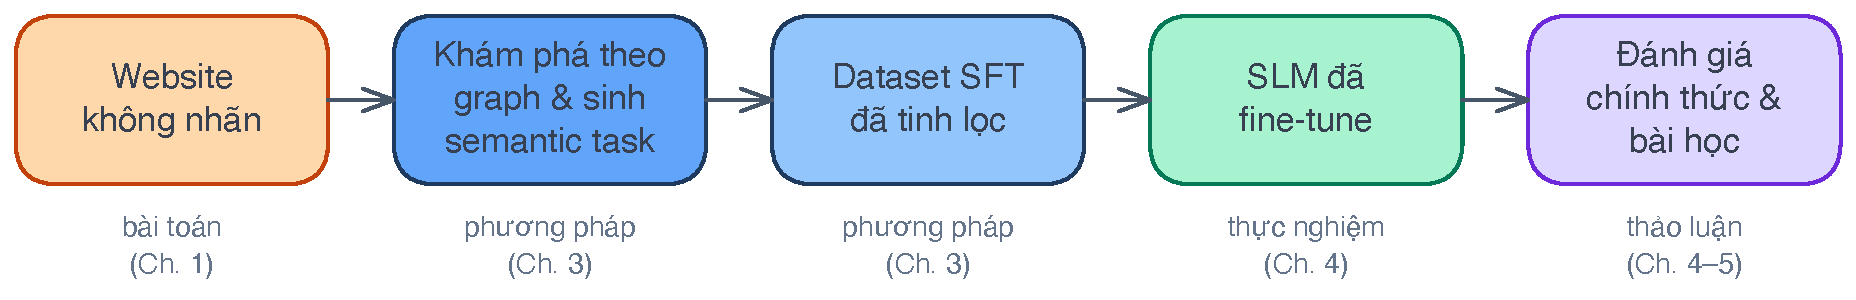
\includegraphics[width=\textwidth]{Figures/fig_roadmap.pdf}
  \caption[Lộ trình nghiên cứu của khóa luận]{Lộ trình nghiên cứu: từ một
    website không nhãn đến một mô hình ngôn ngữ nhỏ được đánh giá chính thức,
  cùng các chương phụ trách từng giai đoạn.}
  \label{fig:bigpicture}
\end{figure}

\vspace{0.5em}
\noindent
Ở chương~2, chúng tôi sẽ đặt lộ trình này vào bức tranh các nghiên cứu hiện có.


\chapter{Kiến thức nền tảng và công trình liên quan}
\label{ch:related}

Chương này (1) giới thiệu bài toán web agent và hạ tầng benchmark dùng
xuyên suốt khóa luận, sau đó khảo sát các công trình liên quan về (2) web
agent dựa trên LLM, (3) khám phá skill và workflow, (4) sinh dữ liệu huấn
luyện tự động cho agent, và (5) mô hình ngôn ngữ nhỏ trong vai trò agent,
trước khi (6) định vị khóa luận so với các hướng nghiên cứu này. Trong mỗi
chủ đề, các công trình được trình bày từ cũ đến mới.

\section{Kiến thức nền tảng}
\label{sec:rel-background}

\subsection{Bài toán web agent}

Một web agent nhận mục tiêu bằng ngôn ngữ tự nhiên và phải hoàn thành nó
bằng cách thao tác website như một người dùng: đọc trang rồi click, gõ và
điều hướng. Trong cách hình thức hóa dạng văn bản đã thành chuẩn, quan sát
là bản tuần tự hóa của accessibility tree, còn action space là một tập nhỏ
các thao tác giao diện có tham số (Mục~\ref{sec:method-graph} nêu bản cụ
thể hóa của chúng tôi). Chính sách của agent thường được xây trên khuôn mẫu
ReAct~\cite{yao2023react}: đan xen suy luận dạng văn bản với hành động, để
mỗi quyết định dựa trên một dòng suy nghĩ tường minh về trạng thái hiện
tại.

\subsection{Benchmark và môi trường}

Hạ tầng đánh giá phát triển theo hướng ngày càng sát thực tế.
WebShop~\cite{yao2022webshop} đưa ra một trang thương mại điện tử mô phỏng
với hơn một triệu sản phẩm thật và các chỉ dẫn mua sắm thu thập từ cộng
đồng; tuy nhiên, nó chỉ có một website đơn giản hóa với một thể loại task.
Mind2Web~\cite{deng2023mind2web} mở rộng lên hơn 2{.}000 task trên 137
website thật, nhưng đánh giá bằng cách phát lại các bản chụp website đã
lưu, nên agent được chấm theo độ khớp với chuỗi hành động ghi sẵn thay vì
theo việc thật sự đạt mục tiêu trong môi trường sống.
WebArena~\cite{zhou2024webarena} khép lại khoảng trống này bằng các bản sao
website đầy đủ chức năng, tự triển khai (một cửa hàng trực tuyến, trang
quản trị của nó, một instance GitLab và một diễn đàn kiểu Reddit), cùng
812 task dài hạn được chấm bằng \emph{bộ chấm tự động} trên trạng thái cuối.
Kết quả chủ đạo của nó định khung cho cả lĩnh vực: agent tốt nhất dựa trên
GPT-4 đạt 14{,}41\% tỷ lệ hoàn thành, so với 78{,}24\% của con người. Khóa
luận này dùng WebArena vừa làm môi trường khám phá vừa làm đích đánh giá
chính thức. Cuối cùng, hệ sinh thái
BrowserGym~\cite{dechezelles2025browsergym} chuẩn hóa giao diện quan sát và
hành động giữa các benchmark; runtime của chúng tôi xây trên nền này.

\subsection{Tinh chỉnh tiết kiệm tham số}

Fine-tune toàn bộ một mô hình 9B tham số vẫn rất tốn bộ nhớ.
LoRA~\cite{hu2022lora} thay vào đó đóng băng trọng số pretrain và chỉ huấn
luyện các ma trận cập nhật hạng thấp cộng thêm, giảm số tham số huấn luyện
đi nhiều bậc mà chất lượng hầu như không đổi; adapter sau đó có thể gộp
ngược vào trọng số gốc để serving. Toàn bộ fine-tuning trong khóa luận dùng
LoRA.

\section{Web agent dựa trên LLM}
\label{sec:rel-llm-agents}

Làn sóng đầu tiên của thời kỳ WebArena cải thiện \emph{kiến trúc agent}
quanh một mô hình lớn cố định. SteP~\cite{sodhi2024step} tổ chức một chồng
(stack) các chính sách LLM, tự động đẩy vào và lấy ra các chính sách con
(đăng nhập, tìm kiếm, điền form) như trạng thái điều khiển; nó vượt xa
baseline nguyên khối của WebArena. Tuy nhiên, thư viện chính sách của SteP
được thiết kế thủ công cho từng họ website, tái nhập chính công sức con
người mà lĩnh vực đang muốn loại bỏ.
AgentOccam~\cite{yang2024agentoccam} cho thấy chỉ cần tinh chỉnh cẩn thận
không gian quan sát và hành động, không cần bất kỳ bộ máy lập kế hoạch
nào, đã vượt nhiều hệ thống cầu kỳ đương thời trên WebArena, một minh
chứng tỉnh táo rằng phần lớn ``tiến bộ agent'' thực ra là kỹ thuật giao
diện. Tuy nhiên, cả hai hướng đều chung hai đặc điểm cấu trúc: chúng coi mô
hình là hàng hóa cố định (thường là hạng GPT-4, trả phí theo lời gọi), và
không để lại sản phẩm bền vững nào: những gì học được về một website
không sống sót qua episode. Với người vận hành cần agent rẻ, riêng tư và
cải thiện được, prompt khéo hơn trên mô hình độc quyền không giải quyết
ràng buộc; nó củng cố ràng buộc.

\section{Khám phá skill và workflow}
\label{sec:rel-skills}

Ý tưởng agent nên tích lũy các hành vi tái sử dụng có gốc rễ sâu. Khung
options~\cite{sutton1999options} hình thức hóa một skill thành bộ ba (tập
khởi đầu, chính sách, điều kiện kết thúc), còn STRIPS~\cite{fikes1971strips}
cho thấy các năng lực mô tả bằng precondition và effect hỗ trợ lập kế hoạch
ký hiệu, cả hai khung hình thức mà HSGE kế thừa trực tiếp
(Mục~\ref{sec:method-graph}).

Trong kỷ nguyên LLM, Voyager~\cite{wang2024voyager} minh họa việc học skill
suốt đời trong Minecraft: một thư viện ngày càng lớn các skill dạng mã thực
thi, mỗi skill được kiểm chứng bằng thực thi trước khi thu nhận. Tuy nhiên,
môi trường của nó có chân lý nền lập trình được (trạng thái game) mà
website không có, và skill của nó phục vụ runtime của một agent chứ không
phục vụ pipeline huấn luyện nào.
Synapse~\cite{zheng2024synapse} lưu nguyên trajectory làm mẫu (exemplar) và
truy xuất theo độ tương đồng để đưa vào prompt. Tuy nhiên, bộ nhớ
trajectory là phẳng: các mẫu không ghép được với nhau, và không gì phân
biệt một trajectory đã kiểm chứng với một trajectory ăn may.
Agent Workflow Memory~\cite{wang2024awm} rút ra các quy trình lặp lại
(workflow) từ trajectory quá khứ rồi tiêm vào prompt các lần sau, cải thiện
đáng kể tỷ lệ thành công trên WebArena. Tuy nhiên, workflow được lưu dưới
dạng văn bản phẳng, thu nhận không qua cổng kiểm chứng tường minh, và chỉ
được tiêu thụ như gợi ý lúc chạy; mô hình bên dưới không hề tốt lên.
Gần đây nhất, skill induction dạng lập trình~\cite{wang2025asi} nâng các
chuỗi hành động lặp lại thành hàm thực thi được, kiểm chứng ngay khi dùng,
ghép các hành động nguyên thủy thành những lời gọi ở mức cao hơn.
SkillWeaver~\cite{zheng2025skillweaver} đi xa hơn: agent tự khám phá, luyện
tập và tinh luyện skill thành các API gọi được thông qua khám phá lặp, cải
thiện đáng kể hiệu năng WebArena nhờ tái sử dụng và thậm chí chuyển giao
skill giữa các agent. Tuy nhiên, ở tất cả các hệ thống này, skill sinh ra
đều phục vụ việc tái sử dụng lúc suy luận bởi một mô hình lớn; không hệ nào
biến cấu trúc skill thành \emph{dữ liệu huấn luyện}.

HSGE đi theo hướng ngược lại: skill được phát hiện và kiểm chứng trên cùng
tinh thần, nhưng mục đích của chúng là được nâng thành các operator lập kế
hoạch mà các phép ghép chuỗi sẽ \emph{sinh ra} những task dài hạn để huấn
luyện một mô hình nhỏ.

\section{Sinh dữ liệu huấn luyện tự động cho agent}
\label{sec:rel-datagen}

Hướng nghiên cứu gần khóa luận nhất là sinh dữ liệu huấn luyện agent không
cần gán nhãn thủ công, phân nhánh theo nguồn dữ liệu.

\subsection{Từ tri thức gián tiếp}

Synatra~\cite{ou2024synatra} chuyển tri thức gián tiếp (các bài hướng
dẫn, tài liệu hướng dẫn thao tác trên mạng) thành bản mẫu tổng hợp ở quy mô lớn, tạo
ra 100k trajectory với chi phí thấp. Tuy nhiên, các bản mẫu được dựng
offline, không hề chạm vào website sống, nên không gì bảo đảm chúng thực
thi được trên môi trường thật.
AgentTrek~\cite{xu2024agenttrek} cải thiện độ bám thực tế bằng cách phát
lại các bài hướng dẫn web trong trình duyệt thật, có VLM kiểm chứng từng
lần phát lại. Tuy nhiên, độ phủ của nó bị chặn bởi những gì đã có bài hướng
dẫn: các quy trình chưa ai viết ra (bao gồm mọi thứ đặc thù của một
website riêng hoặc mới triển khai) nằm ngoài tầm với.

\subsection{Từ khám phá tự động}

Họ thứ hai, giống HSGE, để agent tự khám phá môi trường đích và chế tạo
task từ những gì tìm thấy.
NNetNav~\cite{murty2024nnetnav} khám phá website rồi gán nhãn hồi tố các
episode tương tác bằng chỉ dẫn, cắt tỉa những nhánh không chấp nhận nhãn
sub-task có nghĩa; fine-tune Llama-3.1-8B trên các bản mẫu này đạt trên
16\% trên WebArena. Tuy nhiên, khám phá là các rollout không cấu trúc:
những gì agent học được về năng lực của website bị vứt bỏ thay vì tích lũy,
mỗi episode lại bắt đầu từ con số không.
OS-Genesis~\cite{sun2024osgenesis} áp cùng ý tưởng tổng hợp ngược cho
trajectory GUI: tương tác trước, suy ra task sau. Tuy nhiên, task được suy
theo từng chuỗi tương tác, không có cơ chế ghép các năng lực phát hiện ở
các episode khác nhau.
PAE~\cite{zhou2024pae} khép vòng bằng học tăng cường: một bộ đề xuất task,
một chính sách hành động và một VLM đánh giá mà phán quyết trở thành phần
thưởng. Tuy nhiên, việc đề xuất task chỉ dựa trên ngữ cảnh cục bộ, và RL
trên phần thưởng nhị phân thưa vừa ngốn mẫu vừa nặng hạ tầng so với SFT.
InSTA~\cite{trabucco2025insta} đẩy công thức này lên bề rộng internet, sinh
task cho 150k website sống bằng LLM ở cả khâu sinh lẫn khâu chấm. Tuy
nhiên, bề rộng đánh đổi với chiều sâu: một lượt quét qua nhiều website
không thể khám phá các task nhiều bước, ghép nhiều năng lực, vốn đòi hỏi
tri thức bền vững về một website.
WebRL~\cite{qi2025webrl} tiến hóa một curriculum từ chính các thất bại của
agent, huấn luyện các mô hình mở trên WebArena-Lite với mức cải thiện mạnh,
còn WebAgent-R1~\cite{wei2025webagentr1} huấn luyện mô hình mở đầu--cuối
bằng học tăng cường nhiều lượt trên các rollout song song. Tuy nhiên, cả
hai đều giả định sẵn một phân phối task ban đầu để cải thiện, và vòng tự
tiến hóa của chúng cần bộ máy RL trực tuyến mà SFT tránh được. Một hướng bổ
trợ thay hẳn website sống: WebEvolver~\cite{fang2025webevolver} đồng tiến
hóa một world model với agent để sinh rollout tổng hợp mà không chạm môi
trường thật. Tuy nhiên, một trình mô phỏng học được thừa kế độ phủ của dữ
liệu đã huấn luyện nó, và trajectory của nó chỉ đáng tin ngang độ trung
thực của world model.

Gần khóa luận nhất, Go-Browse~\cite{gandhi2026gobrowse} đóng khung việc thu
thập dữ liệu thành tìm kiếm trên graph của một website: các trang đã thăm
trở thành các node thăm lại được, nên khám phá tái sử dụng thông tin giữa
các episode. Một mô hình 7B fine-tune trên dữ liệu thu được đạt 21{,}7\%
trên WebArena, state of the art cho mô hình dưới 10B tại thời điểm công
bố. Go-Browse xác nhận đúng tiền đề cốt lõi của khóa luận: khám phá
\emph{có cấu trúc} thắng rollout không cấu trúc về chất lượng dữ liệu. Tuy
nhiên, graph của nó là graph \emph{của các trang}, và task của nó vẫn là
các đề xuất bám trang được giải từ những trang đó. HSGE bổ sung một tầng
thứ hai mà Go-Browse không xây: các skill đã kiểm chứng được nâng thành
operator lập kế hoạch với precondition/effect chuẩn hóa. Các chuỗi đi qua
những operator đó sinh ra \emph{semantic task}: những mục tiêu trải dài
trên các năng lực phát hiện ở các episode khác nhau, điều mà không đề xuất
bám trang nào tạo ra được (Mục~\ref{sec:method-semantic}).

\section{Mô hình ngôn ngữ nhỏ trong vai trò agent}
\label{sec:rel-slm}

Luận điểm rằng mô hình nhỏ xứng đáng được đầu tư ngày càng được phát biểu
tường minh: một position paper gần đây~\cite{belcak2025slm} lập luận rằng
phần lớn các lời gọi agent đều hẹp và lặp lại, khiến SLM (rẻ hơn mười
đến ba mươi lần khi serving và fine-tune được trong vài giờ) là nền tảng
hợp lý về kinh tế cho các hệ thống agent.
Về thực nghiệm, AutoWebGLM~\cite{lai2024autowebglm} xây một web agent triển
khai được trên backbone 6B thông qua SFT theo curriculum và học theo sở
thích. Tuy nhiên, dữ liệu huấn luyện của nó khởi động từ các mẫu gán nhãn
thủ công và curriculum dựng tay. Các hệ thống dựa trên khám phá ở mục trước
cung cấp đúng nguồn dữ liệu còn thiếu: mô hình 8B của NNetNav và 7B của
Go-Browse cho thấy bản mẫu thu thập tự động dịch chuyển đáng kể mô hình nhỏ
trên WebArena, còn WebRL đẩy xa hơn bằng RL. Tuy nhiên, xuyên suốt các công
trình này, nút thắt nhất quán là pipeline dữ liệu chứ không phải bộ tối ưu
và đó chính là thành phần khóa luận thiết kế lại. Mô hình đích của
chúng tôi là Qwen3.5-9B, một mô hình trọng số mở gần đây mà họ mô hình được
tài liệu hóa trong báo cáo kỹ thuật Qwen3~\cite{yang2025qwen3}.

\section{Định vị khóa luận}
\label{sec:rel-positioning}

Bảng~\ref{tab:positioning} định vị HSGE theo năm trục: dữ liệu có đến từ
tương tác sống với website đích không; khám phá có được cấu trúc hóa bằng
một biểu diễn bền vững không; skill tái sử dụng có được kiểm chứng trước
khi dùng lại không; task dài hạn có được sinh bằng cách \emph{ghép} các
năng lực đã khám phá không; và pipeline có huấn luyện một mô hình nhỏ
không.

\begin{table}[H]
\centering
\caption[Định vị HSGE so với các hệ thống liên quan gần nhất]{Định vị HSGE
so với các hệ thống liên quan gần nhất. \CIRCLE{} = có,
\LEFTcircle{} = một phần, - = không.}
\label{tab:positioning}
\small
\begin{tabular}{@{}L{3.2cm} C{1.7cm} C{2.0cm} C{1.9cm} C{2.1cm} C{1.6cm}@{}}
\toprule
\textbf{Hệ thống} & \textbf{Tương tác sống} & \textbf{Khám phá có cấu trúc}
& \textbf{Skill kiểm chứng} & \textbf{Task dài hạn ghép chuỗi}
& \textbf{Huấn luyện SLM} \\
\midrule
Synapse~\cite{zheng2024synapse} & - & - & - & - & - \\
AWM~\cite{wang2024awm} & \CIRCLE & - & - & - & - \\
ASI~\cite{wang2025asi} & \CIRCLE & - & \CIRCLE & \LEFTcircle & - \\
SkillWeaver~\cite{zheng2025skillweaver} & \CIRCLE & - & \CIRCLE & \LEFTcircle & - \\
Synatra~\cite{ou2024synatra} & - & - & - & - & \CIRCLE \\
AgentTrek~\cite{xu2024agenttrek} & \CIRCLE & - & - & - & \CIRCLE \\
NNetNav~\cite{murty2024nnetnav} & \CIRCLE & - & - & - & \CIRCLE \\
OS-Genesis~\cite{sun2024osgenesis} & \CIRCLE & - & - & - & \CIRCLE \\
PAE~\cite{zhou2024pae} & \CIRCLE & - & - & - & \CIRCLE \\
WebRL~\cite{qi2025webrl} & \CIRCLE & \LEFTcircle & - & - & \CIRCLE \\
Go-Browse~\cite{gandhi2026gobrowse} & \CIRCLE & \CIRCLE & - & - & \CIRCLE \\
\textbf{HSGE (của chúng tôi)} & \CIRCLE & \CIRCLE & \CIRCLE & \CIRCLE & \CIRCLE \\
\bottomrule
\end{tabular}
\end{table}

Tóm lại, hướng kiến trúc agent chủ yếu cải thiện chiến lược prompting và điều phối quanh các mô hình lớn cố định. Phương pháp khám phá kỹ năng có khả năng tích lũy tri thức có cấu trúc, nhưng phần lớn chỉ sử dụng tri thức này trong giai đoạn suy luận. Trong khi đó, phương pháp sinh dữ liệu hướng đến huấn luyện mô hình nhỏ thường thực hiện khám phá theo cách thiếu cấu trúc hoặc chỉ tổ chức thông tin ở cấp độ trang. Theo hiểu biết của chúng tôi, hướng tiếp cận kết hợp các kỹ năng đã được kiểm chứng, ghép chúng thành các tác vụ ngữ nghĩa dài hạn và sử dụng những tác vụ này để huấn luyện mô hình ngôn ngữ nhỏ vẫn chưa được nghiên cứu đầy đủ. Đây chính là khoảng trống mà khóa luận hướng đến giải quyết.


\vspace{1em}
\noindent
Chương tiếp theo trình bày phương pháp lấp vào vị trí đó.


\chapter{Phương pháp đề xuất}
\label{ch:method}

Chương này trình bày chi tiết về HSGE (Hierarchical Skill-Graph Exploration) -- chuỗi xử lý (pipeline) do nhóm nghiên cứu đề xuất nhằm chuyển đổi một website chưa được gán nhãn thành tập dữ liệu huấn luyện cho các mô hình ngôn ngữ nhỏ. Nội dung chương được cấu trúc thành các phần chính bao gồm: (1) tổng quan về pipeline và các nguyên tắc thiết kế lõi; (2) cơ chế biểu diễn đồ thị hai tầng làm nền tảng cho toàn bộ phương pháp; (3) quá trình khám phá có định hướng dựa trên đồ thị thông qua các tác vụ mức thấp (low-level task) do LLM đề xuất; (4) phương pháp phát hiện và kiểm chứng các kỹ năng (skill) có khả năng tái sử dụng; (5) cơ chế sinh các tác vụ ngữ nghĩa (\emph{semantic task}) dài hạn thông qua việc ghép chuỗi các toán tử (operator) lập kế hoạch; (6) quy trình tinh lọc quỹ đạo tương tác (trajectory) để xây dựng tập dữ liệu tinh chỉnh (fine-tuning); (7) thực hiện tinh chỉnh mô hình SLM mục tiêu; và cuối cùng là (8) một số ghi chú trong quá trình cài đặt và hiện thực hóa hệ thống.

\section{Tổng quan}
\label{sec:method-overview}

Đầu vào của hệ thống HSGE là một website đang hoạt động nhưng chưa được gán nhãn tác vụ (task), kết hợp cùng một biên khám phá (frontier) được khởi tạo từ một hoặc một vài URL hạt giống. Đầu ra là một tập dữ liệu tinh chỉnh có giám sát (SFT) bao gồm các quỹ đạo tương tác (trajectory) hướng mục tiêu, và sản phẩm cuối cùng là một mô hình ngôn ngữ nhỏ đã được tinh chỉnh (fine-tuned) trên tập dữ liệu này. Hình~\ref{fig:pipeline} thể hiện kiến trúc tổng thể của hệ thống.

\begin{figure}[htbp]
\centering
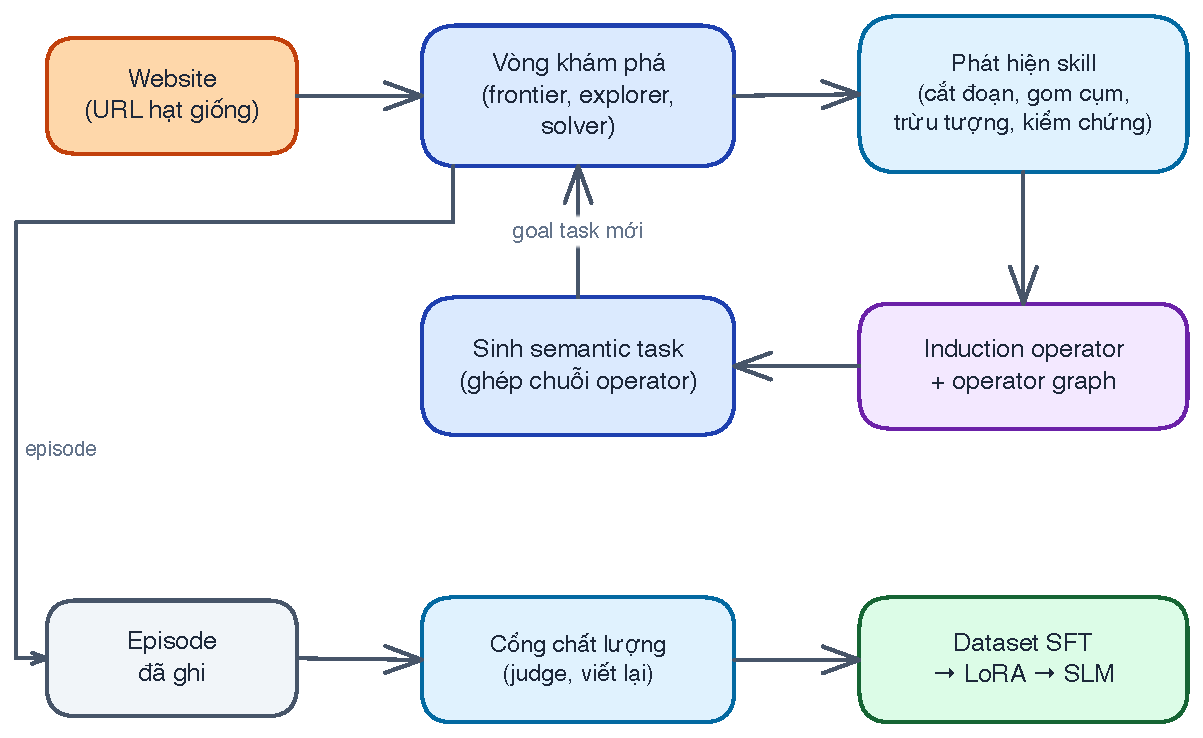
\includegraphics[width=\textwidth]{Figures/fig_pipeline.pdf}
\caption[Tổng quan pipeline HSGE]{Tổng quan chuỗi xử lý (pipeline) HSGE. Vòng lặp khám phá thực thi các tác vụ mức thấp (low-level task) do LLM đề xuất trên các trang thuộc frontier; các kỹ năng (skill) phát hiện được sẽ được nâng cấp thành các toán tử (operator) lập kế hoạch, sau đó quá trình ghép chuỗi các toán tử này sẽ tạo ra các tác vụ ngữ nghĩa (semantic task) để phản hồi ngược lại cho vòng khám phá. Mọi phiên tương tác (episode) được ghi nhận đều phải vượt qua các cổng kiểm duyệt chất lượng tự động trước khi trở thành dữ liệu huấn luyện.}
\label{fig:pipeline}
\end{figure}

Chuỗi xử lý (pipeline) này vận hành dưới dạng một vòng lặp khép kín. Tại mỗi trang được truy cập, một mô-đun khám phá (\emph{explorer}) sẽ đề xuất các tác vụ cụ thể gắn liền với nội dung của trang đó. Tiếp theo, một tác nhân giải quyết (\emph{solver} agent) sẽ thử nghiệm thực thi các tác vụ này trên trình duyệt thực, qua đó tạo ra các quỹ đạo tương tác. Thành phần phát hiện (discovery) chịu trách nhiệm phân cắt các quỹ đạo này thành từng đoạn nhỏ, gom cụm các đoạn có tính lặp lại, rồi trừu tượng hóa những cụm đã đạt độ chín thành các kỹ năng (\emph{skill}) có khả năng tái sử dụng.

Kế tiếp, hệ thống nâng cấp các skill đã qua kiểm chứng thành các toán tử (\emph{operator}) lập kế hoạch với điều kiện tiên quyết (precondition) và hiệu ứng (effect) được xác định rõ ràng. Quá trình ghép chuỗi các toán tử trên đồ thị sẽ kiến tạo nên các tác vụ mục tiêu dài hạn, được gọi là tác vụ ngữ nghĩa (\emph{semantic task}). Các tác vụ này sau đó được đưa ngược lại cho chính solver, tạo thành một vòng lặp khép kín. Mọi tác vụ được thử nghiệm, bất kể ở mức thấp hay mức ngữ nghĩa, đều được ghi nhận thành một phiên (episode). Các episode này còn phải vượt qua những cổng kiểm duyệt chất lượng tự động trước khi được biên dịch thành tập dữ liệu SFT phục vụ cho quá trình tinh chỉnh SLM mục tiêu.

Trong một lượt chạy, ba loại phiên tương tác được ghi nhận và được đánh dấu
riêng biệt, vì chúng khác nhau về điểm xuất phát chứ không chỉ về nội dung tác
vụ. Phiên \texttt{LOCAL} là một tác vụ mức thấp được giải ngay tại trang đang
xét, tức tác nhân đã đứng sẵn ở đúng nơi cần thao tác. Phiên
\texttt{UNPREFIXED} là chính tác vụ đó được giải lại một lần nữa từ trang chủ,
nên quỹ đạo bao gồm cả phần điều hướng tìm đường (Mục~\ref{sec:method-unprefixed}).
Phiên \texttt{GOAL} là một tác vụ ngữ nghĩa nhiều bước, sinh từ chuỗi operator
hoặc từ seed năng lực của website (Mục~\ref{sec:method-semantic}). Ba nhãn này
đi theo dữ liệu tới tận bước dựng tập huấn luyện, nơi chúng trở thành ba mức
độ khó của curriculum.

Quá trình thiết kế pipeline được định hướng bởi ba nguyên tắc xuyên suốt:

\begin{itemize}
  \item \textbf{P1: Kiểm chứng trước khi tái sử dụng.} Không có thông tin nào được mặc nhiên tin cậy ngay ở lần xuất hiện đầu tiên. Một skill chỉ được hệ thống thu nhận sau khi chứng minh được tính lặp lại qua các trajectory độc lập; một trạng thái tự tuyên bố thành công phải được đánh giá lại bởi một mô-đun giám khảo (judge) độc lập; và một toán tử sẽ bị loại bỏ nếu hiệu ứng của nó rỗng nghĩa.
  \item \textbf{P2: Cấu trúc đồ thị thay vì bộ nhớ phẳng.} Thay vì lưu trữ thông tin dưới dạng một tập hợp rời rạc các trang hoặc bộ nhớ phẳng, HSGE duy trì một cấu trúc đồ thị hai tầng (Mục~\ref{sec:method-graph}). Tầng thấp ghi nhận \emph{vị trí} agent đã từng đi qua; trong khi tầng cao ghi nhận những \emph{hành động} agent có thể thực hiện, cũng như cách thức các năng lực này liên kết với nhau.
  \item \textbf{P3: Hệ thống tác vụ hai tầng.} Các tác vụ mức thấp (\emph{low-level task}) do LLM đề xuất (Mục~\ref{sec:method-exploration}) đóng vai trò định hướng quá trình khám phá và cung cấp nguyên liệu thô cho việc phát hiện skill. Trong khi đó, các tác vụ ngữ nghĩa (\emph{semantic task}) (Mục~\ref{sec:method-semantic}) biểu diễn những mục tiêu nhiều bước mà không một trang web đơn lẻ nào có thể trực tiếp gợi ý. Tầng ngữ nghĩa được cấp bởi hai nguồn độc lập nhau: ghép chuỗi các năng lực đã kiểm chứng theo hướng từ dưới lên, và seed năng lực của website theo hướng từ trên xuống. Việc duy trì đồng thời hai nguồn là một quyết định thiết kế có chủ đích, xuất phát từ thực nghiệm: nguồn từ dưới lên chỉ hoạt động khi đồ thị toán tử đã có cạnh, một điều kiện thưa hơn dự kiến rất nhiều (Mục~\ref{sec:disc-operators}).
\end{itemize}

\section{Biểu diễn đồ thị hai tầng}
\label{sec:method-graph}

Hình~\ref{fig:twolevel} minh họa cấu trúc biểu diễn được đề xuất trong mục này. Tầng thấp ghi lại quá trình tương tác thực tế: các trang web mà agent đã truy cập và những hành động nó thực hiện giữa các trang đó. Tầng cao lưu trữ các năng lực có khả năng tái sử dụng: các kỹ năng (skill) được trừu tượng hóa từ quá trình tương tác, cùng với các cạnh toán tử (operator) chỉ ra cách thức chúng có thể được ghép nối với nhau.

\begin{figure}[htbp]
\centering
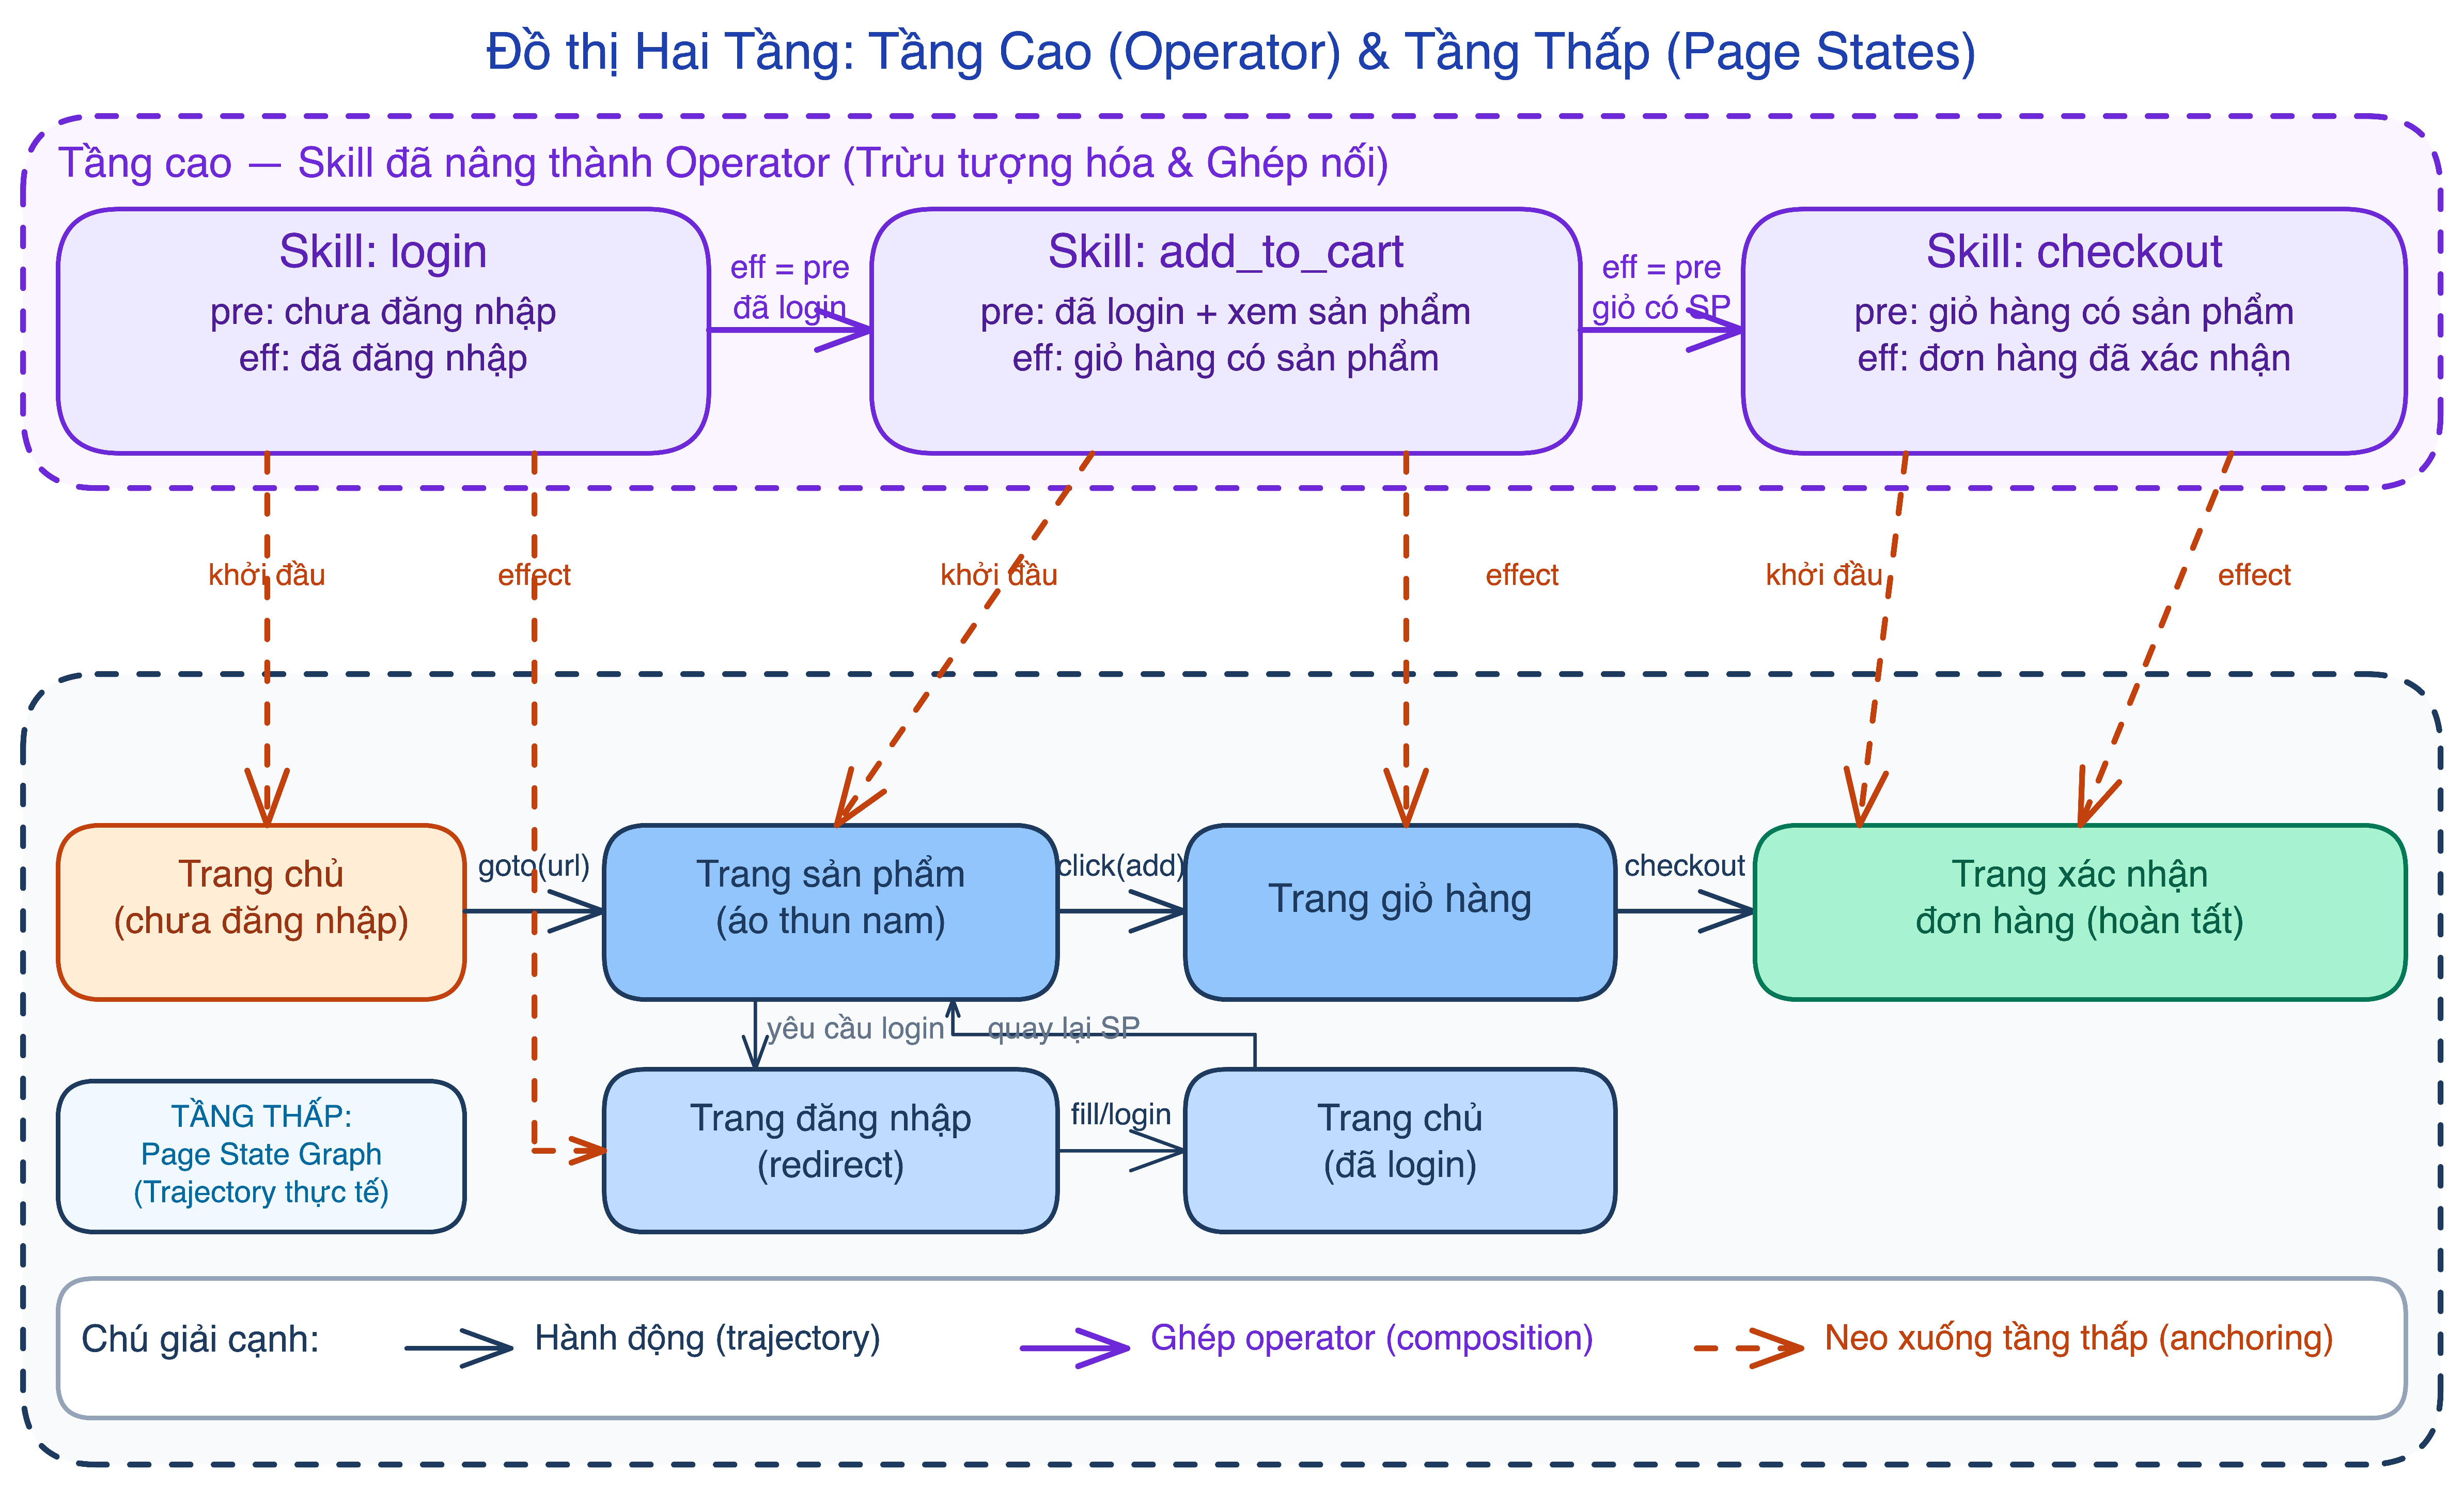
\includegraphics[width=0.95\textwidth]{Figures/fig_twolevel.pdf}
\caption[Đồ thị hai tầng]{Đồ thị hai tầng. Tầng thấp ghi nhận các trạng thái trang (page state) đã thăm và các cạnh quỹ đạo tương tác (hành động) giữa chúng; tầng cao biểu diễn các skill được nâng cấp thành các operator lập kế hoạch và nối với nhau bằng các cạnh ghép (nơi effect của operator trước khớp với precondition của operator sau). Các skill được neo vào tầng thấp thông qua các liên kết trừu tượng hóa và initiation/effect.}
\label{fig:twolevel}
\end{figure}

\subsection{Mô hình hóa website như một quá trình quyết định}

Chúng tôi mô hình hóa website như một Quá trình Quyết định Markov quan sát được một phần (POMDP)~\cite{kaelbling1998pomdp}: agent không bao giờ nhìn thấy toàn bộ trạng thái của máy chủ, mà chỉ thấy phần giao diện đang được hiển thị. Tại mỗi bước, agent nhận được một quan sát $o = (u, x)$, trong đó $u$ là URL hiện tại và $x$ là \emph{cây trợ năng} (accessibility tree - axtree) của trang. Axtree đóng vai trò như một bản tuần tự hóa dưới dạng văn bản (text serialization) của các phần tử giao diện đang hiển thị, trong đó mỗi phần tử được gắn một mã định danh ổn định.

Cách biểu diễn quan sát bằng axtree và việc quy các thao tác giao diện về một tập lệnh hữu hạn không phải là đóng góp của khóa luận: đây là quy ước chuẩn của WebArena~\cite{zhou2024webarena} và bộ công cụ BrowserGym~\cite{dechezelles2025browsergym} mà HSGE kế thừa. Trên nền đó, agent tương tác với môi trường thông qua một không gian hành động cố định $\mathcal{A}$ (Bảng~\ref{tab:actions}). Không gian này gồm các thao tác với phần tử, điều hướng, quản lý tab và hai hành động kết thúc phiên: trả lời người dùng hoặc tuyên bố tác vụ bất khả thi. Một \emph{quỹ đạo tương tác} (trajectory) là chuỗi $\tau = \langle (o_0, a_0), (o_1, a_1), \dots \rangle$ được sinh ra trong quá trình thực thi một tác vụ.

\begin{table}[H]
\centering
\caption[Action space của solver]{Không gian hành động của solver. Các đối số phần tử tham chiếu mã định danh hiển thị trong accessibility tree. Nhóm ba hành động không tác động lên trạng thái trang được tách riêng vì chúng chỉ tồn tại để gỡ bế tắc thao tác, và về sau chính sự phân biệt này quyết định một cổng lọc dữ liệu (Mục~\ref{sec:method-data}).}
\label{tab:actions}
\small
\begin{tabular}{@{}L{5.4cm} L{7.8cm}@{}}
\toprule
\textbf{Hành động} & \textbf{Ý nghĩa} \\
\midrule
\texttt{click(id)} & Nhấn vào phần tử \texttt{id}. \\
\texttt{fill(id, text)} & Nhập chuỗi \texttt{text} vào ô \texttt{id}. \\
\texttt{select\_option(id, opt)} & Chọn tùy chọn \texttt{opt} trong danh sách thả xuống \texttt{id}. \\
\texttt{press(id, key)} & Gửi phím tắt đến phần tử \texttt{id}. \\
\texttt{goto(path)}, \texttt{go\_back()} & Điều hướng tới một đường dẫn \emph{tương đối} trên chính website hiện tại / Quay lại trang trước. \\
\texttt{new\_tab()}, \texttt{tab\_focus(i)}, \texttt{tab\_close()} & Quản lý tab trình duyệt. \\
\addlinespace
\texttt{scroll(dx, dy)} & Cuộn trang; dùng để đưa một phần tử ngoài khung nhìn vào trạng thái thao tác được. \\
\texttt{hover(id)} & Di chuột lên phần tử \texttt{id}. \\
\texttt{noop(ms)} & Chờ trang ổn định. \\
\addlinespace
\texttt{send\_msg\_to\_user(text)} & Kết thúc: Phản hồi câu trả lời hoặc báo cáo hoàn thành. \\
\texttt{report\_infeasible(reason)} & Kết thúc: Khẳng định tác vụ không thể thực hiện. \\
\bottomrule
\end{tabular}
\end{table}

Ba hành động \texttt{scroll}, \texttt{hover} và \texttt{noop} vốn được lớp
thực thi hỗ trợ ngay từ đầu nhưng ban đầu không được mô tả trong prompt, nên
mô hình không bao giờ dùng tới. Hệ quả là khi một thao tác thất bại vì phần tử
chưa ở trạng thái sẵn sàng, phương án duy nhất mà mô hình còn lại là nhấn
lại chính phần tử đó. Việc bổ sung chúng vào tài liệu hành động, kèm chỉ dẫn
tường minh rằng một lỗi quá hạn chờ nghĩa là phần tử có tồn tại nhưng chưa
thao tác được, là một sửa chữa xuất phát từ số liệu của lần chạy thật
(Mục~\ref{sec:exp-analysis}).

Một chi tiết khác của không gian hành động là \texttt{goto} luôn nhận đường
dẫn tương đối. Địa chỉ máy chủ của một bản triển khai WebArena chỉ là ngẫu
nhiên của nơi nó được dựng lên, trong khi dữ liệu của khóa luận được thu thập
trên một máy chủ và được đánh giá trên một máy chủ hoàn toàn khác. Vì vậy, mọi
URL xuất hiện trong prompt cũng như mọi đích đến của \texttt{goto} đều được
lược bỏ phần gốc (origin) trước khi hiển thị hoặc trước khi trở thành đích
huấn luyện, và phần gốc của trang hiện tại chỉ được ghép trở lại ngay trước
thời điểm hành động được thực thi. Phép biến đổi hai chiều này được áp dụng
thống nhất ở cả ba nơi (solver lúc chạy thật, bộ dựng dataset và bộ viết lại
suy nghĩ), nhờ đó một hành động \texttt{goto} học được trên một bản triển khai
vẫn chạy đúng trên một bản triển khai khác.

\subsection{Tầng thấp: Trạng thái trang và cạnh quỹ đạo}

Tầng thấp của đồ thị lưu giữ các bước tương tác cụ thể: các node đại diện cho những trạng thái trang đã thăm (được định danh bởi URL và giá trị băm (hash) của axtree ban đầu); các cạnh thể hiện những hành động mà agent đã thực sự thực thi giữa các trạng thái đó. Việc băm (hashing) nội dung trang thay vì chỉ dựa vào URL là một cơ chế thiết yếu trong thực tế: hai URL khác nhau thường trỏ đến cùng một nội dung giao diện; nếu chỉ dùng URL, việc thăm lại chúng sẽ làm lãng phí ngân sách khám phá vào những nội dung mà agent đã biết.

\subsection{Tầng cao: Biểu diễn skill như các option}

Một \emph{skill} được định nghĩa là một hành vi có khả năng tái sử dụng và được tham số hóa. Khái niệm này được hình thức hóa dựa trên khung options~\cite{sutton1999options} thành bộ ba $\sigma = \langle I, \pi, \beta \rangle$: tập khởi đầu $I$ (các trạng thái trang mà skill có thể được kích hoạt), chính sách $\pi$ (thủ tục hành động) và điều kiện kết thúc $\beta$. Cụ thể, HSGE biểu diễn mỗi skill thông qua một \emph{thẻ kỹ năng} (skill card). Thẻ này gồm tên, mô tả bằng ngôn ngữ tự nhiên, danh sách các tham số được định kiểu (ví dụ: chuỗi tìm kiếm hoặc giá trị điền form), cùng các liên kết trỏ về những đoạn quỹ đạo thành phần mà từ đó skill được trừu tượng hóa. Các node skill kết nối với trạng thái ở tầng thấp thông qua cạnh khởi đầu và cạnh hiệu ứng, đồng thời nối kết với nhau thông qua cạnh ghép chuỗi để hình thành nên đồ thị tầng cao.

\subsection{Toán tử lập kế hoạch: Precondition và Effect}

Việc lập kế hoạch trực tiếp trên các skill thô là không khả thi do điều kiện áp dụng của chúng chỉ tồn tại ở dạng ngầm định. Do đó, HSGE nâng cấp mỗi skill đã qua kiểm chứng thành một toán tử (\emph{operator}) theo mô hình STRIPS cổ điển~\cite{fikes1971strips}: $\omega = \langle \mathit{pre}, \mathit{eff} \rangle$. Ở đây $\mathit{pre}$ và $\mathit{eff}$ là các tập mệnh đề bằng ngôn ngữ tự nhiên, chẳng hạn ``người dùng đang xem danh sách issue của một dự án''.

Điểm khác biệt so với các bộ lập kế hoạch truyền thống là từ vựng của các mệnh đề không được cố định từ trước. Thay vào đó, các mệnh đề này do LLM tự sinh trong quá trình quy nạp (induction), sau đó được \emph{chuẩn hóa} thành các mã định danh ổn định thông qua một bộ gom cụm dựa trên vector nhúng (embedding) (Mục~\ref{sec:method-semantic}). Cơ chế này đảm bảo rằng các cách diễn đạt khác nhau của cùng một điều kiện sẽ được quy về một mệnh đề duy nhất. Trên nền đó, một \emph{đồ thị toán tử} (operator graph) sẽ hình thành một cạnh nối từ $\omega_1$ sang $\omega_2$ khi một hiệu ứng (effect) của $\omega_1$ thỏa mãn điều kiện tiên quyết (precondition) của $\omega_2$. Các đường đi trên đồ thị này chính là các kế hoạch đa kỹ năng (multi-skill) có thể thực thi được.

\subsection{Phân loại thuật ngữ tác vụ}

Xuyên suốt khóa luận, chúng tôi định nghĩa hai phân cấp tác vụ riêng biệt. \emph{Tác vụ mức thấp} (low-level task) là những chỉ dẫn ngắn, gắn liền với một trang web cụ thể do mô-đun explorer đề xuất trong quá trình thăm trang (ví dụ: ``mở merge request được cập nhật gần nhất''). Ngược lại, \emph{tác vụ ngữ nghĩa} (semantic task) là những mục tiêu dài hạn được kiến tạo từ đồ thị toán tử bằng cách ghép chuỗi ít nhất hai operator. Loại tác vụ này phụ thuộc hoàn toàn vào cấu trúc của đồ thị và chính là sản phẩm cốt lõi của phương pháp đề xuất.

\section{Khám phá có định hướng theo đồ thị}
\label{sec:method-exploration}

Quá trình khám phá tại mỗi bước cần giải quyết ba câu hỏi cốt lõi: di chuyển đến \emph{đâu} tiếp theo, thử nghiệm \emph{điều gì} tại đó, và thực thi \emph{như thế nào}. Hệ thống HSGE phân bổ ba nhiệm vụ này lần lượt cho các thành phần: biên khám phá (frontier), mô-đun đề xuất (explorer) và tác nhân giải quyết (solver).

\subsection{Quản lý frontier}
\label{sec:method-frontier}

\begin{figure}[htbp]
\centering
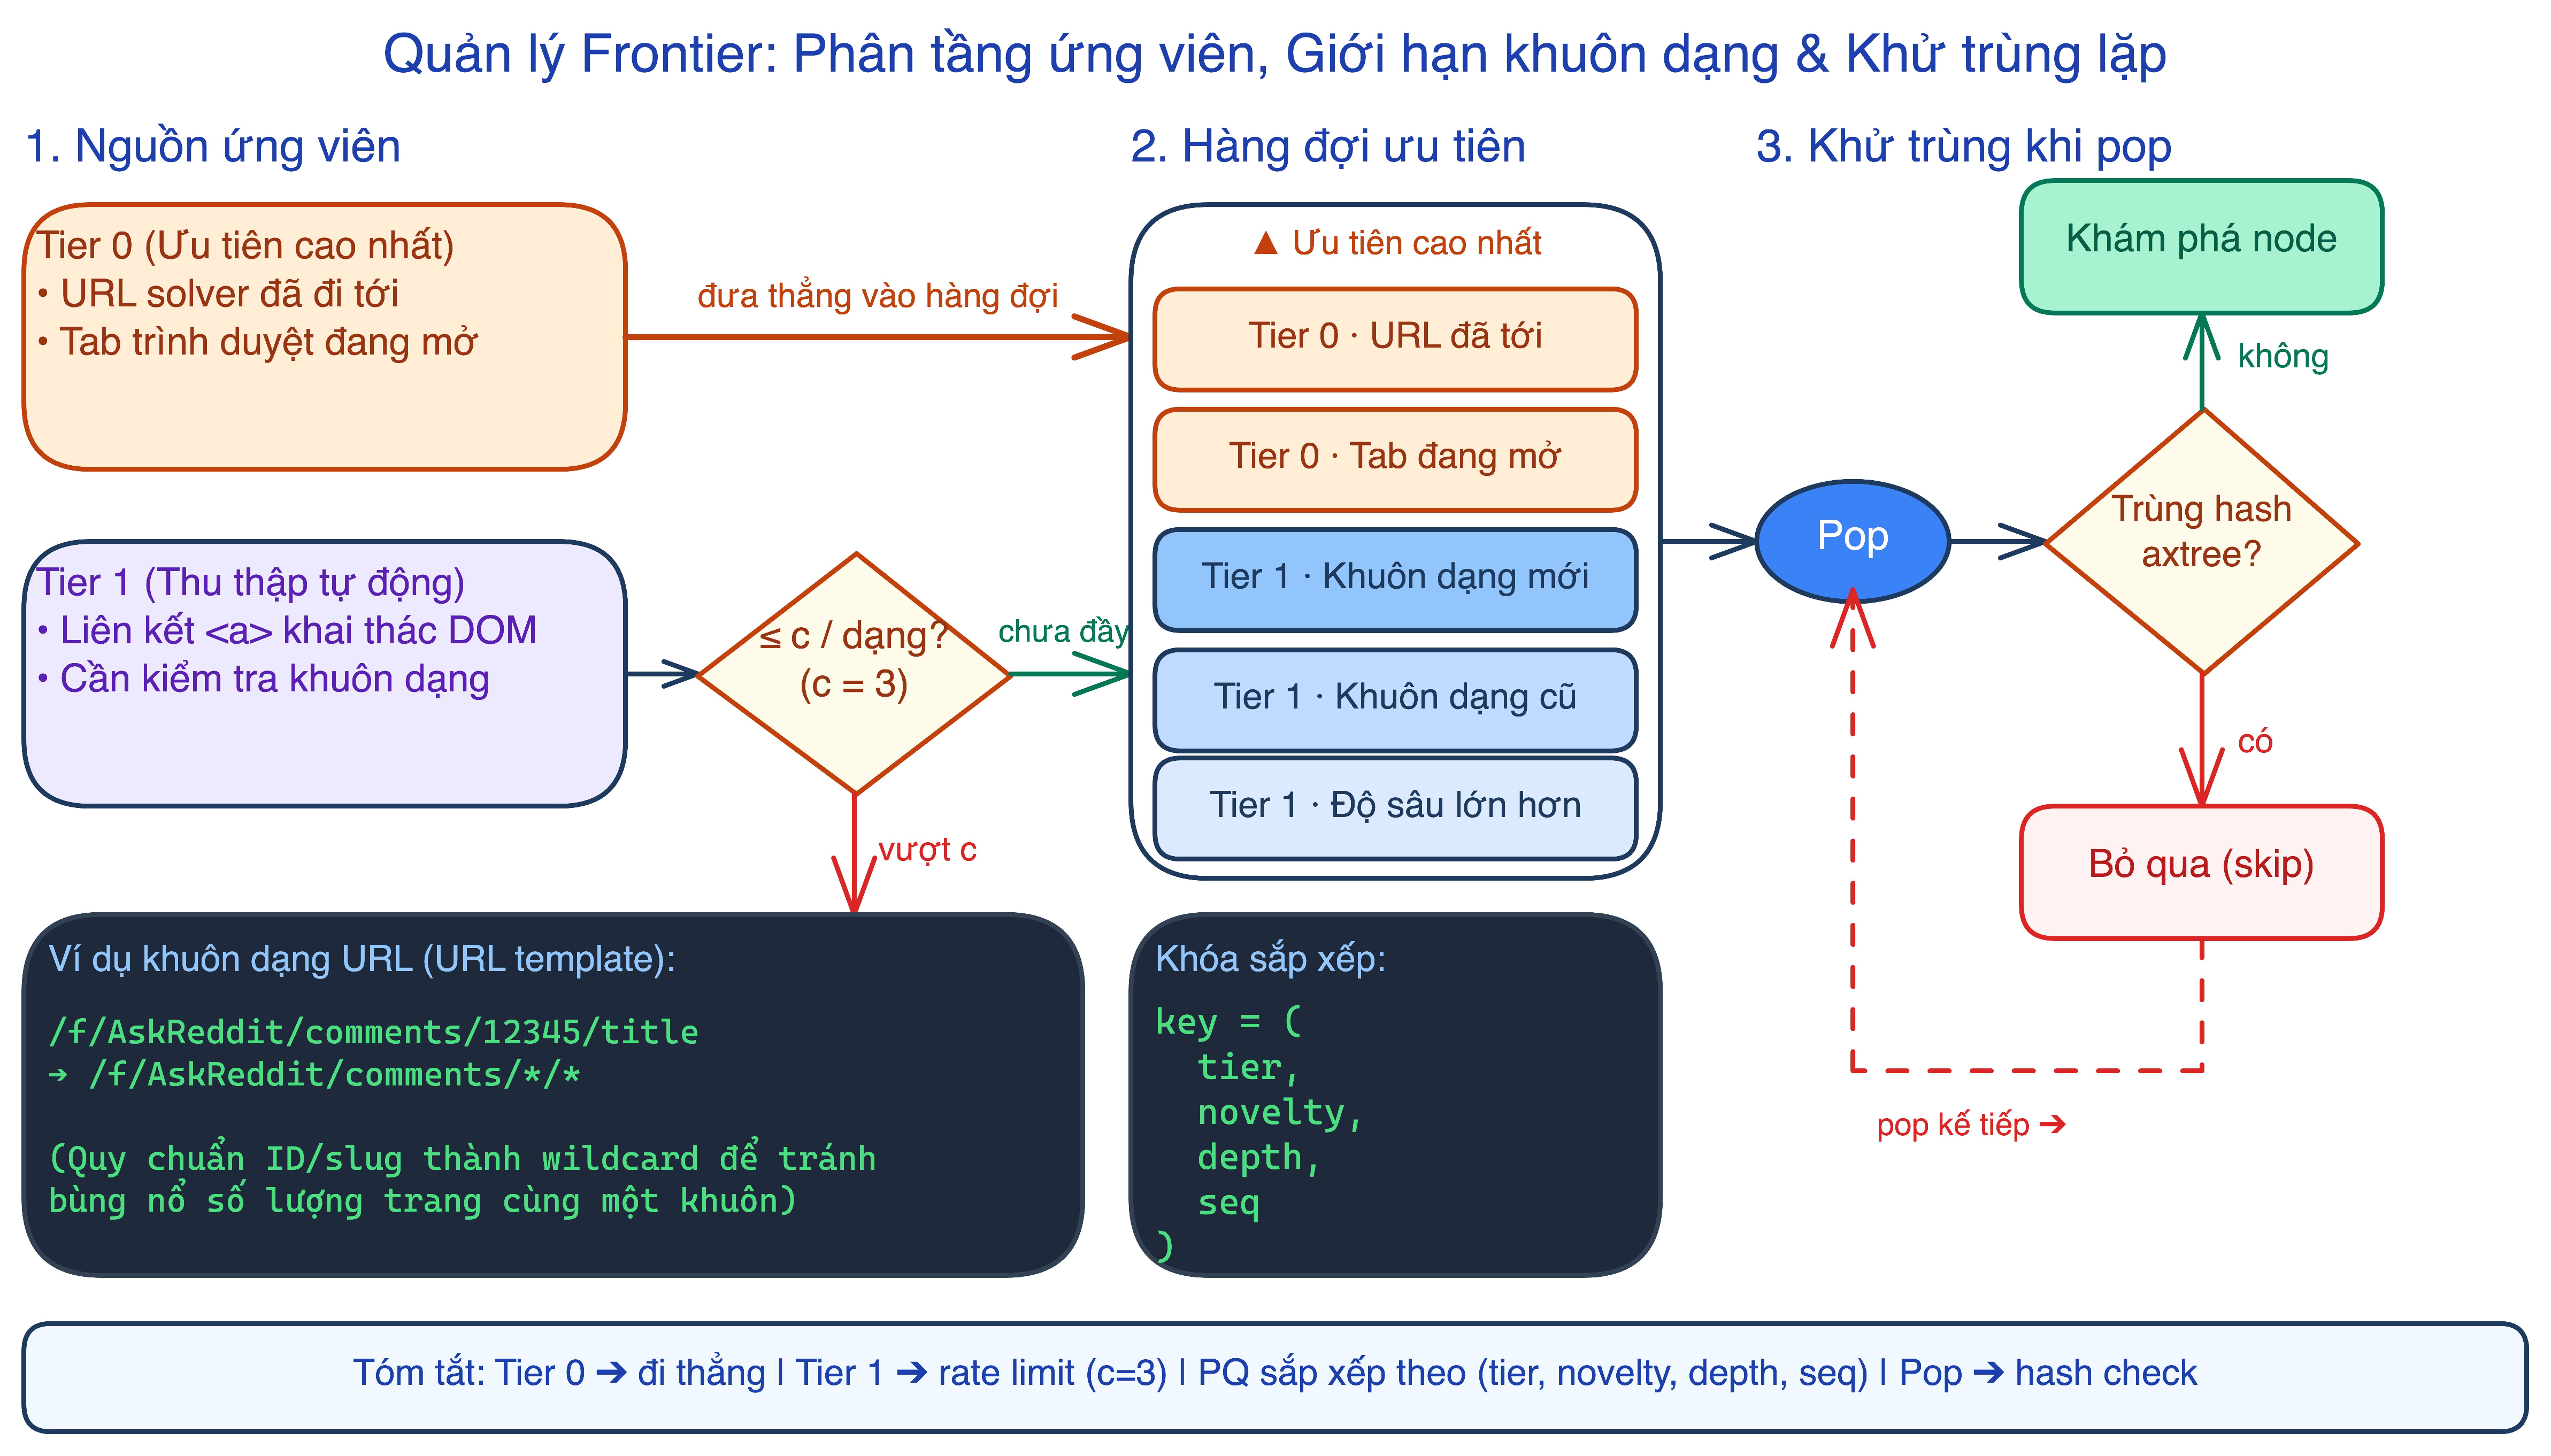
\includegraphics[width=\textwidth]{Figures/fig_frontier.pdf}
\caption[Quản lý frontier]{Quản lý frontier. Hai tầng ứng viên được xử lý theo các cơ chế khác nhau: URL mà solver thực tế đã truy cập được đưa trực tiếp vào hàng đợi, trong khi các siêu liên kết (hyperlink) khai thác từ trang phải vượt qua rào lọc theo khuôn dạng (template). Hàng đợi sắp xếp các ứng viên ưu tiên theo tầng, tiếp đến là độ mới của định dạng URL, và cuối cùng là độ sâu. Một node khi được lấy ra vẫn sẽ bị bỏ qua nếu nội dung trang có giá trị băm (hash) trùng lặp với một trang đã thăm trước đó.}
\label{fig:frontier}
\end{figure}

Frontier được cấu trúc như một hàng đợi ưu tiên dành cho các URL ứng viên, phân làm hai tầng (Hình~\ref{fig:frontier}). \emph{Tầng 0} bao gồm các URL mà agent thực tế đã truy cập khi giải quyết tác vụ, cùng với các trang đang mở trên tab; việc agent truy cập thành công bản thân nó đã là minh chứng cho mức độ liên quan của trang, nên nhóm này luôn được lấy ra trước. \emph{Tầng 1} lưu trữ các siêu liên kết được trích xuất từ cấu trúc DOM của mỗi trang đã thăm. Việc khai thác hyperlink là bắt buộc; nếu không, sự mở rộng của biên khám phá sẽ phụ thuộc hoàn toàn vào các thao tác điều hướng sinh ra khi giải quyết tác vụ. Điều này dẫn đến một rủi ro hệ thống (sẽ được phân tích kỹ hơn ở Chương~\ref{ch:discussion}): nếu một trang web chỉ bao gồm các tác vụ tra cứu thông tin, nó sẽ không cung cấp thêm bất kỳ URL mới nào cho biên khám phá.

Tuy nhiên, số lượng liên kết được trích xuất thường rất ồ ạt và dễ bị áp đảo bởi các trang có cấu trúc tương đồng (ví dụ: mọi bài đăng, bình luận, trang cá nhân trên một diễn đàn thường dùng chung một khuôn mẫu trang). Để ngăn chặn tình trạng quá tải hàng đợi, mỗi URL sẽ được chuẩn hóa thành một \emph{khuôn dạng URL} (URL template): loại bỏ giao thức (scheme), chuỗi truy vấn (query) và phân mảnh (fragment); các đoạn đường dẫn đóng vai trò định danh cùng mọi thành phần phía sau sẽ được thay thế bằng ký tự đại diện. Ví dụ:
\begin{center}
\texttt{/f/AskReddit/comments/12345/title}
$\;\rightarrow\;$
\texttt{/f/AskReddit/comments/*/*}.
\end{center}
Mỗi template chỉ được phép truy cập tối đa $c$ trang; các lượt chạy trong khóa luận dùng $c = 3$ cho tầng 1, và toàn bộ tham số chạy cùng giá trị đã dùng được liệt kê ở Phụ lục~\ref{app:design-params}. Giới hạn này được kiểm tra theo cơ chế đánh giá lười (lazy evaluation) ngay tại thời điểm lấy URL ra khỏi hàng đợi, bởi tần suất xuất hiện của một template sẽ tăng dần theo thời gian chạy (run). Tại tầng 1, các ứng viên thuộc template chưa từng gặp sẽ được ưu tiên trước, tiếp đến là các trang ở mức nông hơn, và cuối cùng là thứ tự chèn.

Điểm cần nói rõ là tầng 0 cũng chịu một trần theo template, chỉ với giá trị
rộng hơn ($c = 8$), chứ \emph{không} được miễn trừ. Việc miễn trừ hoàn toàn cho
tầng 0 là thiết kế ban đầu và nó đã hỏng theo một cách khá đặc trưng: khi
solver giải một tác vụ bên trong một chuỗi bình luận, mọi URL nó chạm tới trong
lúc giải đều được đẩy lên đầu hàng đợi mà không qua bộ lọc nào, khiến một
diễn đàn duy nhất chiếm 58 trên 158 node của một lượt chạy thật. Nói cách khác,
bằng chứng ``agent đã đi tới đó'' đủ để \emph{ưu tiên} một trang, nhưng không
đủ để cho nó quyền chiếm ngân sách khám phá không giới hạn.

Thuật toán~\ref{alg:frontier} tóm tắt vòng lặp này. Việc chống trùng lặp được
thực hiện ở ba mức khác nhau, vì cùng một trang có thể xuất hiện dưới ba dạng
khác nhau. Thứ nhất, mỗi URL được chuẩn hóa (bỏ phân mảnh, hạ chữ thường phần
giao thức và tên máy, bỏ dấu gạch chéo cuối) trước khi đối chiếu với tập đã
thăm; chuỗi truy vấn được \emph{giữ lại}, bởi hai giá trị truy vấn khác nhau
thường thực sự là hai trang khác nhau. Thứ hai, sau khi trình duyệt điều hướng
xong, URL thực tế mà nó dừng lại cũng được đối chiếu, để bắt các trường hợp
chuyển hướng về một trang đã thăm. Thứ ba, mã băm nội dung của cây trợ năng
ban đầu được đối chiếu, để bắt những URL khác nhau nhưng hiển thị nội dung
giống hệt. Node nào trùng theo một trong ba mức đều bị bỏ qua, vì thăm lại nó
tiêu tốn trọn một lô lời gọi LLM mà không mang lại phát hiện nào.

\begin{algorithm}[H]
\caption{Vòng khám phá có định hướng theo đồ thị}
\label{alg:frontier}
\begin{algorithmic}[1]
\State $F \gets$ hàng đợi ưu tiên khởi tạo với URL hạt giống $r$; $V \gets \emptyset$
\While{$F \neq \emptyset$ \textbf{và} chưa vượt quá ngân sách node}
  \State $u \gets \textsc{Pop}(F)$ \Comment{khóa: (tầng, độ mới template, độ sâu, thứ tự)}
  \If{template của $u$ đã đạt trần của tầng đó} \textbf{continue} \EndIf
  \State $o \gets \textsc{Load}(u)$ \Comment{lỗi tải trang: ghi log, bỏ qua node, không dừng run}
  \If{$\textsc{Landed}(o) \in V$ \textbf{hoặc} $\textsc{Hash}(o) \in V$} \textbf{continue} \EndIf
  \State $V \gets V \cup \{\textsc{Landed}(o), \textsc{Hash}(o)\}$
  \State $D \gets \emptyset$ \Comment{các task đã giải được tại node này}
  \For{task $t \in \textsc{Explorer}(o)$} \Comment{low-level task, Mục~\ref{sec:method-lowlevel}}
    \State $\tau \gets \textsc{Solver}(u, t)$; ghi episode nhãn \texttt{LOCAL}
    \If{$\tau$ thành công} $\textsc{Discovery}(\tau)$; $D \gets D \cup \{t\}$ \EndIf
    \State thêm các URL đạt tới trong $\tau$ vào $F$ ở tầng 0
  \EndFor
  \For{task $t \in D$} \Comment{lấy mẫu không tiền tố, Mục~\ref{sec:method-unprefixed}}
    \State $\tau \gets \textsc{Solver}(r, t)$; ghi episode nhãn \texttt{UNPREFIXED}
    \If{$\tau$ thành công} $\textsc{Discovery}(\tau)$ \EndIf
  \EndFor
  \For{task $t \in \textsc{SemanticTasks}(u)$} \Comment{chuỗi operator + seed, Mục~\ref{sec:method-semantic}}
    \State $\tau \gets \textsc{Solver}(u, t)$; ghi episode nhãn \texttt{GOAL}
  \EndFor
  \State khai thác hyperlink của $u$; thêm vào tầng 1 theo trần template
  \State ghi sản phẩm trung gian và điểm kiểm tra (checkpoint) của node
\EndWhile
\end{algorithmic}
\end{algorithm}

\subsection{Đề xuất tác vụ mức thấp (low-level task)}
\label{sec:method-lowlevel}

Tại mỗi trang thuộc biên khám phá, một mô-đun \emph{explorer} vận hành lõi LLM sẽ đề xuất tối đa $k$ tác vụ cụ thể gắn liền với nội dung trang; giá trị mặc định là $k = 6$, còn các lượt chạy thu thập dữ liệu của khóa luận dùng $k = 9$ (Phụ lục~\ref{app:design-params}). Các đề xuất này được biểu diễn dưới dạng dữ liệu có cấu trúc, đi kèm trường phân loại tường minh nhận một trong bốn giá trị: \texttt{INFO} (tra cứu một thông tin), \texttt{NAV} (đi tới một trang cụ thể), \texttt{MOD} (thay đổi nội dung hoặc trạng thái) và \texttt{COMPOSITE} (một mục tiêu tự thân đòi hỏi nhiều thao tác mới thỏa mãn, chẳng hạn ``mua con chuột không dây rẻ nhất còn hàng''). Cách làm này thay cho việc yêu cầu LLM trả về văn bản tự do (free-text) kèm thẻ gắn phân loại -- một quy ước mà thử nghiệm trên website thật cho thấy mô hình không tuân thủ ổn định (Mục~\ref{sec:disc-guardrails}).

Nhóm \texttt{COMPOSITE} có vai trò riêng và được prompt yêu cầu đặt lên đầu danh sách: đây là nhóm duy nhất trong bốn nhóm mà một tác vụ đơn lẻ đã trải qua nhiều trạng thái trang, nên nó là nguồn sinh ra các kỹ năng có thể tái sử dụng và ghép chuỗi. Một quy tắc cụ thể đi kèm là khi trang hiện tại có biểu mẫu nhiều trường, explorer không được đề xuất tác vụ chỉ điền một trường đơn lẻ, mà phải đề xuất một tác vụ hoàn tất trọn vẹn biểu mẫu đó theo đúng mục đích của nó. Ngoài ra, mọi tác vụ liên quan tới tài khoản và xác thực (đăng nhập, đăng xuất, đăng ký, đổi mật khẩu, xóa tài khoản) đều bị cấm tuyệt đối ở mọi chế độ, bởi phiên làm việc vốn đã được xác thực sẵn và tài khoản được dùng chung giữa các lượt chạy.

Việc phân loại đóng vai trò then chốt đối với chế độ \emph{chỉ đọc} (read-only) dành cho các website dùng chung. Ở chế độ này, các tác vụ \texttt{MOD} cũng như mọi tác vụ mô hình không phân loại được đều bị loại bỏ theo nguyên tắc an toàn đóng mặc định (fail-closed), nhằm phòng ngừa những tác vụ thay đổi trạng thái bị ngụy trang.

Hệ thống áp dụng ba cơ chế để kiểm soát thành phần và tính đa dạng của danh sách đề xuất. Thứ nhất, explorer duy trì trạng thái xuyên suốt toàn bộ quá trình chạy và ghi nhớ mọi tác vụ đã từng đề xuất; các đề xuất gần nhất sẽ được đưa ngược lại vào prompt dưới dạng ngữ cảnh phủ định (negative context), đồng thời các phiên bản gần trùng lặp sẽ bị loại bỏ ở cấp độ mã nguồn. Thiếu đi cơ chế này, một tỷ lệ lớn các đề xuất sẽ thoái hóa thành những lệnh điều hướng menu lặp lại trên mọi trang (Mục~\ref{sec:disc-exploration}).

Thứ hai, hai nhóm tác vụ bị giới hạn số lượng \emph{không điều kiện}, bất kể ngân sách $k$ còn trống hay không: tối đa một tác vụ \texttt{NAV} và tối đa hai tác vụ \texttt{INFO} cho mỗi trang. Lý do của trần \texttt{NAV} là các tác vụ \texttt{COMPOSITE} và \texttt{MOD} vốn đã tự điều hướng sang trang mới trong lúc thao tác, nên một tác vụ điều hướng thuần túy chỉ cần giữ lại như một khoản dự phòng. Lý do của trần \texttt{INFO} đến từ số liệu của một lượt chạy thật: khi nhóm này chỉ bị cắt lúc danh sách vượt ngân sách, các trang đề xuất ít tác vụ sẽ để lọt toàn bộ \texttt{INFO}, và kết quả là \texttt{INFO} chiếm 49\% tổng số phiên thành công, trong đó phần lớn kết thúc bằng một câu trả lời mà không có bất kỳ thao tác trình duyệt nào. Đó là dữ liệu dạy mô hình \emph{trả lời}, không phải dạy mô hình \emph{hành động}, nên nó cần được giữ ở mức vừa đủ chứ không phải càng nhiều càng tốt.

Thứ ba, khi danh sách vẫn vượt quá $k$ sau hai bước trên, thứ tự giữ lại được quy định tường minh: trước hết là một lượng \texttt{COMPOSITE} dự trữ, rồi tới toàn bộ \texttt{MOD}, rồi một lượng \texttt{INFO} dự trữ, rồi \texttt{NAV}, và sau cùng mới tới phần \texttt{COMPOSITE} dôi ra, các tác vụ không phân loại được và phần \texttt{INFO} dôi ra. Trật tự này bảo đảm cả hai điều: nhóm sinh ra skill không bao giờ bị cắt hết, còn nhóm chỉ đọc luôn giữ được một phần đại diện trong dữ liệu.

Khi seed năng lực của website đã được suy ra (Mục~\ref{sec:method-seed}), mô tả website cùng danh sách năng lực còn được đưa vào prompt của explorer như ngữ cảnh bổ sung, kèm chỉ dẫn rằng chúng không được thay thế các tác vụ gắn với trang hiện tại. Mục đích là để các tác vụ mức thấp bám sát mục đích thật của website, thay vì chỉ mô tả những gì trang đang hiển thị.

Các tác vụ đề xuất này được \emph{chủ đích} giữ ở mức thấp: mỗi tác vụ nằm trọn vẹn trong phạm vi chức năng của một trang đơn lẻ. Vai trò cốt lõi của chúng là tạo ra các quỹ đạo tương tác đa dạng, đóng vai trò là nguồn dữ liệu thô để từ đó hệ thống trích xuất các kỹ năng, và sau cùng là nền tảng để tổng hợp thành các tác vụ ngữ nghĩa.

\subsection{Tác nhân giải quyết (Solver)}
\label{sec:method-solver}

\begin{figure}[htbp]
\centering
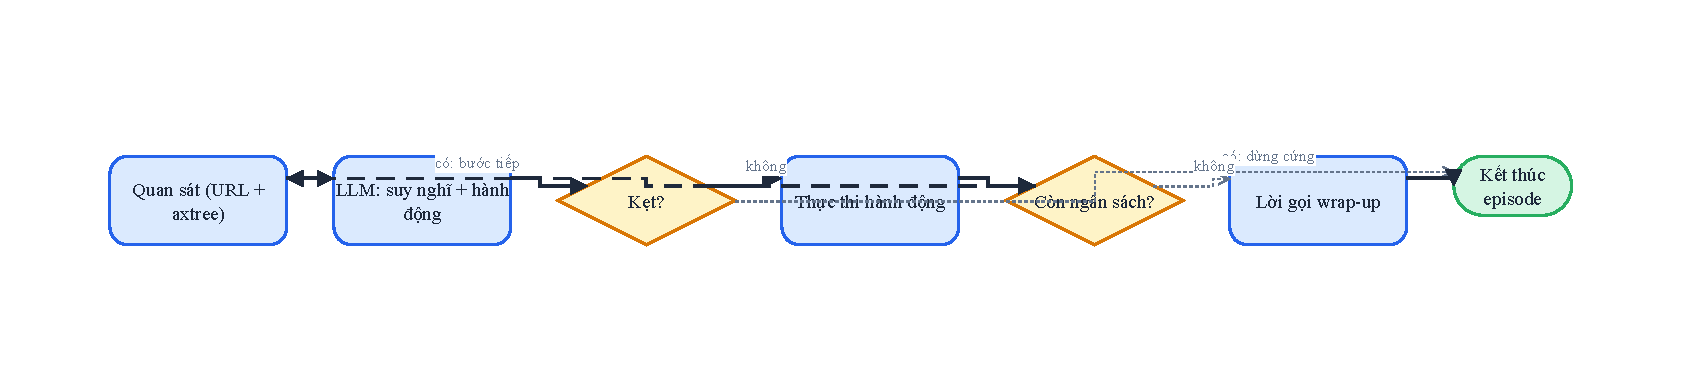
\includegraphics[width=\textwidth]{Figures/fig_solver.pdf}
\caption[Vòng lặp Solver với chốt chặn cấu trúc]{Vòng lặp quan sát, suy nghĩ, hành động của solver. Cơ chế chốt chặn vòng lặp kẹt (stuck-loop) sẽ chấm dứt ngay episode khi các hành động liên tục lặp lại trên cùng một đối tượng đích mà không tạo ra bất kỳ sự thay đổi quan sát nào; khi cạn kiệt ngân sách bước nhảy, hệ thống gọi một hàm tổng kết (wrap-up) duy nhất, chỉ cho phép tuyên bố hoàn thành hoặc báo cáo bất khả thi.}
\label{fig:solver}
\end{figure}

\emph{Solver} hoạt động dựa trên vòng lặp agent theo kiến trúc ReAct~\cite{yao2023react}, được phác họa ở Hình~\ref{fig:solver}. Tại mỗi bước, nó tiếp nhận mục tiêu, URL hiện tại (dạng tương đối), cây trợ năng (đã được giới hạn ở 6000 ký tự, kèm dấu hiệu cắt tường minh), một mục báo lỗi của hành động liền trước, và một khung cửa sổ chứa sáu hành động gần nhất. Mỗi hành động trong cửa sổ đó đều đi kèm kết quả quan sát được (``đang ở $\langle$url$\rangle$'', ``trang đã đổi'', ``không đổi'', hoặc ``hành động thất bại: $\langle$lỗi$\rangle$'') nhằm giúp mô hình phân biệt được sự tiến triển so với việc không tạo ra tiến triển. Mục báo lỗi \emph{luôn hiện diện} trong prompt và mang giá trị ``(none)'' khi không có lỗi, thay vì chỉ xuất hiện ở những bước hiếm hoi có lỗi; nhờ vậy nó là một phần cố định của định dạng mà mô hình học cách tra cứu. Tiếp theo, solver đưa ra dòng suy luận và thực thi một hành động thuộc Bảng~\ref{tab:actions}.

Một hành động bị lớp thực thi từ chối vẫn được ghi vào lịch sử như mọi hành động khác, với kết quả là ``thất bại'' và không có tiến triển. Chi tiết này quan trọng hơn vẻ ngoài của nó: trước đây một hành động lỗi được bỏ qua hoàn toàn, khiến cả hai cơ chế chống lặp bên dưới không nhìn thấy gì, và trong một lượt chạy thật đã có 118 phiên tiêu trọn ngân sách để phát đi phát lại một cú nhấp mà phần tử đích không bao giờ ở trạng thái thao tác được.

Vòng lặp của solver được kiểm soát bởi ba cơ chế chốt chặn cấu trúc, mỗi cơ chế bắt một dạng bế tắc khác nhau.

\textbf{Chốt chặn theo đối tượng đích.} Solver theo dõi xem mỗi hành động có làm thay đổi quan sát hay không và tác động lên đối tượng đích nào. Một chuỗi các hành động cuối cùng nhắm vào \emph{cùng một đối tượng đích} mà \emph{không tạo ra sự thay đổi quan sát} trước hết sẽ kích hoạt một cảnh báo chèn thẳng vào prompt (sau hai lần), rồi tới một lệnh chấm dứt lập tức (hard stop) nếu hành vi vẫn tiếp diễn (sau bốn lần). Thiết kế hai mức này xuất phát từ một quan sát trên website thật: cảnh báo bằng văn bản không đủ để mô hình ngừng click vào một phần tử trơ (unresponsive), như trình bày ở Mục~\ref{sec:disc-guardrails}. Việc ràng buộc thêm yếu tố ``không có sự thay đổi quan sát'', thay vì chỉ so khớp chuỗi hành động, giúp cơ chế chốt chặn không bị kích hoạt sai (false positive). Nhờ đó nó không cắt nhầm những chuỗi thao tác hợp lệ cần tái sử dụng một phần tử xuyên suốt nhiều trang khác nhau.

\textbf{Chốt chặn theo độ mới của quan sát.} Cơ chế trên chỉ nhận ra bế tắc khi mô hình lặp lại \emph{cùng} một đối tượng đích. Trong thực tế còn một dạng bế tắc khác, khi mô hình liên tục đổi đối tượng nhưng không bao giờ chạm tới một trang mới, tức nó đang loanh quanh chứ không đang tiến. Vì vậy solver ghi lại tập các quan sát đã đạt tới và đếm số bước liên tiếp không đưa lại quan sát nào mới; vượt qua ngưỡng cảnh báo (bốn bước) thì prompt được chèn một lời nhắc đổi hướng tiếp cận, vượt qua ngưỡng dừng (tám bước) thì episode kết thúc.

\textbf{Lời gọi tổng kết.} Khi vòng lặp kết thúc mà chưa có hành động kết thúc nào được chọn, dù vì cạn ngân sách bước hay vì một trong hai chốt chặn trên, solver thực thi một lời gọi \emph{tổng kết} (wrap-up call) cuối cùng. Lời gọi này thuần túy ở định dạng văn bản và chỉ được phép phản hồi \texttt{send\_msg\_to\_user} (tuyên bố hoàn thành) hoặc \texttt{report\_infeasible} (báo cáo bất khả thi); mọi phản hồi khác đều bị loại bỏ. Một chi tiết đáng lưu ý là prompt tổng kết nói đúng \emph{lý do thật} khiến episode dừng, bởi hai chốt chặn thường bắn sớm hơn ngân sách rất nhiều; nếu vẫn nói với mô hình rằng nó đã cạn ngân sách thì mô hình sẽ chép lại lời đó, và một lượt chạy thật đã ghi nhận những phiên dừng ở bước thứ năm nhưng báo cáo lý do bất khả thi là ``ngân sách hành động đã cạn''.

Lý do dừng này được lưu lại cùng episode, vì nó phân biệt hai tình huống trông giống hệt nhau trong dữ liệu. Một báo cáo bất khả thi mà tác nhân tự đưa ra \emph{trong lúc} đang giải là một kết luận; cũng câu đó nhưng đến từ lời gọi tổng kết sau khi tác nhân đã bị chặn lại chỉ là một lời biện minh sau sự việc. Trạng thái bất khả thi được xem là một kết quả hợp lệ ở mức cao nhất (first-class outcome): nó không bao giờ được thực thi trên trình duyệt, không bao giờ được thử lại và không tham gia vào quá trình phát hiện skill, nhưng loại thứ nhất được giữ lại làm tín hiệu huấn luyện dạy mô hình biết khi nào nên dừng, còn loại thứ hai bị loại khỏi tập dữ liệu (Mục~\ref{sec:method-data}).

Sau cùng, việc tác nhân tự tuyên bố hoàn thành không đủ để một phiên được ghi là thành công nếu tác vụ thuộc nhóm thay đổi trạng thái. Với một tác vụ \texttt{MOD} hoặc \texttt{COMPOSITE}, hệ thống yêu cầu thêm một điều kiện kiểm tra được bằng mã: phải có ít nhất một hành động đã thực sự làm trang thay đổi. Điều kiện này sinh ra từ một phiên thật, nơi tác vụ ``gửi email xác nhận cho đơn hàng \#000000299'' được tuyên bố hoàn thành ngay ở bước đầu tiên, không một thao tác trình duyệt nào, với lý do rằng email ``đã được gửi rồi''. Các tác vụ \texttt{INFO} và \texttt{NAV} không chịu ràng buộc này, bởi trả lời ngay trên trang đích chính là hình dạng đúng của chúng.

Cuối cùng, khi tác vụ là một mục tiêu ngữ nghĩa nhiều bước, solver có thể được vận hành ở chế độ \emph{bám subgoal}: một thành phần lập kế hoạch phân rã mục tiêu thành từ hai tới năm subgoal có thứ tự, và tại mỗi bước prompt chỉ trưng ra subgoal hiện tại kèm yêu cầu chỉ làm việc trên subgoal đó. Con trỏ subgoal tiến lên khi mô hình phát tín hiệu hoàn thành, hoặc tự động tiến sau một số bước trần, và chỉ subgoal cuối cùng mới được phép kết thúc episode.

\subsection{Lấy mẫu không tiền tố (unprefixed sampling)}
\label{sec:method-unprefixed}

Mọi phiên tương tác mô tả cho tới đây đều có \emph{tiền tố}: trước khi giải một
tác vụ, trình duyệt được đưa về đúng trang mà tác vụ đó gắn với, nên tác nhân
bắt đầu ở nơi cần thao tác. Cách làm này là hệ quả tự nhiên của việc explorer
đề xuất tác vụ theo từng trang, nhưng nó tạo ra một sai lệch nghiêm trọng cho
dữ liệu huấn luyện: phần khó nhất của một tác vụ web thật, tức tìm đường tới
đúng trang, đã bị lược bỏ. Số liệu của một lượt chạy thật cho thấy quy mô của
sai lệch đó: 287 trên 465 quỹ đạo thành công chỉ dài đúng \emph{một} bước, vì
tác nhân đã đứng sẵn ở đích ngay từ đầu.

Vì vậy, sau khi hoàn tất toàn bộ tác vụ mức thấp tại một node, hệ thống thực
hiện thêm một lượt \emph{không tiền tố} theo tinh thần của Go-Browse~\cite{gandhi2026gobrowse}:
mỗi tác vụ \emph{đã giải được} ở node đó được giải lại một lần nữa trên một
trình duyệt mới mở tại trang chủ của website. Quỹ đạo thu về vì thế chứa cả
phần điều hướng lẫn phần thao tác, và được ghi nhận với nhãn \texttt{UNPREFIXED}
ở mức độ khó 2. Vì một tác vụ không tiền tố thực chất là tác vụ cũ cộng thêm
phần tìm đường, nó dùng ngân sách bước của nhóm mục tiêu ngữ nghĩa thay vì
ngân sách của tác vụ cục bộ.

Chỉ những tác vụ đã thành công mới được giải lại. Một tác vụ mà tác nhân không
làm nổi ngay cả khi đứng đúng trang thì cũng không dễ hơn khi phải tự tìm
đường tới đó, nên trả tiền hai lần cho nó chỉ làm hao ngân sách. Đổi lại,
lượt không tiền tố có một tác dụng phụ đáng kể đối với khâu phát hiện kỹ năng:
giải cùng một tác vụ từ hai điểm xuất phát khác nhau cũng chính là cách một
cụm quỹ đạo tích đủ số lần tái xuất hiện để đạt độ chín và trở thành skill.

\section{Phát hiện kỹ năng (Skill Discovery)}
\label{sec:method-skills}

Mọi quỹ đạo tương tác (trajectory) sau khi hoàn tất sẽ đi qua chuỗi xử lý (pipeline) phát hiện gồm bốn giai đoạn: phân cắt quỹ đạo, gom cụm, trừu tượng hóa, và kiểm chứng (Hình~\ref{fig:discovery}).

\begin{figure}[htbp]
\centering
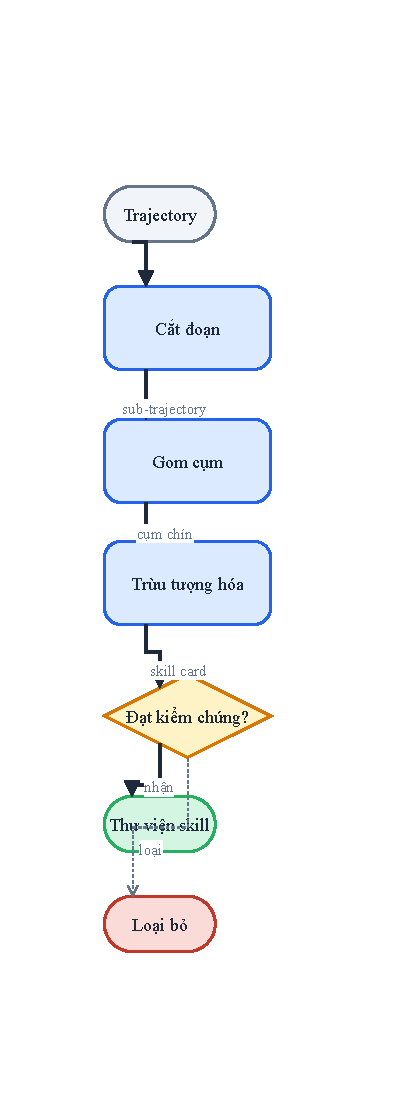
\includegraphics[width=0.48\textwidth]{Figures/fig_discovery.pdf}
\caption[Pipeline phát hiện skill]{Chuỗi xử lý phát hiện kỹ năng. Một trajectory hoàn tất sẽ được phân cắt thành các quỹ đạo con (sub-trajectory), gom cụm, trừu tượng hóa thành thẻ kỹ năng (skill card), và chỉ được lưu vào thư viện nếu vượt qua bước kiểm chứng; nếu không, nó sẽ bị loại bỏ.}
\label{fig:discovery}
\end{figure}

Thuật toán~\ref{alg:discovery} trình bày toàn bộ bốn giai đoạn dưới dạng mã
giả; các mục tiếp theo giải thích chi tiết từng giai đoạn. Điểm cần lưu ý là
pipeline chỉ được kích hoạt trên những quỹ đạo của tác vụ đã giải thành công:
một episode thất bại hoặc kết thúc bằng \texttt{report\_infeasible} không bao
giờ tham gia vào quá trình phát hiện kỹ năng.

\begin{algorithm}[H]
\caption{Phát hiện kỹ năng từ một quỹ đạo tương tác}
\label{alg:discovery}
\begin{algorithmic}[1]
\Require quỹ đạo $\tau$ gồm $n$ bước của một tác vụ đã giải thành công, với
quan sát $o_i = (u_i, x_i)$; thư viện skill $L$; ngưỡng axtree
$\theta_{\mathrm{ax}}$, ngưỡng gom cụm $\theta_{\mathrm{sim}}$, độ chín $m$
\Ensure tập các skill được thu nhận thêm vào $L$
\State $C \gets \emptyset$ \Comment{điểm cắt ứng viên}
\For{$i \gets 1$ \textbf{đến} $n-1$}
  \If{$u_i \neq u_{i-1}$ \textbf{hoặc} $\textsc{Sim}(x_{i-1}, x_i) < \theta_{\mathrm{ax}}$}
    \State $C \gets C \cup \{i\}$
  \EndIf
\EndFor
\State $S \gets \textsc{Arbitrate}(\tau, C)$ \Comment{LLM gộp/xác nhận; điểm cắt không hợp lệ bị bỏ, không phản hồi thì giữ nguyên $C$}
\State $S \gets \textsc{MergeNav}(S)$ \Comment{đoạn một bước thuần điều hướng gộp vào đoạn kề}
\State $A \gets \emptyset$
\For{mỗi quỹ đạo con $\sigma \in S$}
  \State $v \gets \textsc{Embed}(\sigma)$ \Comment{sentence embedding, đã chuẩn hóa $L_2$}
  \State $c \gets \arg\max_j \cos(v, \mu_j)$ \Comment{$\mu_j$ là tâm cụm $j$}
  \If{$L$ chưa có cụm nào \textbf{hoặc} $\cos(v, \mu_c) < \theta_{\mathrm{sim}}$}
    \State $c \gets$ cụm mới, tâm khởi tạo bằng $v$
  \Else
    \State thêm $\sigma$ vào cụm $c$; cập nhật $\mu_c$ theo trung bình lũy tiến rồi chuẩn hóa lại
  \EndIf
  \If{$|\textsc{Members}(c)| \ge m$ \textbf{và} $c$ chưa được trừu tượng hóa}
    \State đánh dấu $c$ đã trừu tượng hóa
    \State $\mathit{card} \gets \textsc{Abstract}(\textsc{Members}(c))$ \Comment{LLM sinh skill card}
    \If{$\textsc{Verify}(\mathit{card})$}
      \State $L \gets L \cup \{\mathit{card}\}$; \; $A \gets A \cup \{\mathit{card}\}$
    \EndIf
  \EndIf
\EndFor
\State \Return $A$
\end{algorithmic}
\end{algorithm}

\subsection{Phân cắt quỹ đạo (Segmentation)}

Một quỹ đạo tương tác thường là sự đan xen của nhiều hành vi khác nhau (như tìm kiếm, lọc, và mở kết quả). Bước phân cắt sẽ chia trajectory ban đầu thành các \emph{quỹ đạo con} (sub-trajectory) có tính liền mạch và đồng nhất về mặt ngữ nghĩa. Các điểm phân cắt tiềm năng (candidate cut points) được xác định dựa trên hai tín hiệu: sự thay đổi của URL và sự sụt giảm độ tương đồng giữa hai cây trợ năng (accessibility tree) liên tiếp. Tín hiệu thứ hai giúp hệ thống nắm bắt được các chuyển đổi trạng thái ngay bên trong một trang (ví dụ: một hộp thoại pop-up xuất hiện) mà không làm thay đổi URL. Sau đó, một LLM sẽ đóng vai trò phân xử các điểm cắt tiềm năng này để đưa ra quyết định gộp hoặc xác nhận phân cắt. Kết quả đầu ra sẽ được kiểm tra tính hợp lệ so với tập ứng viên ban đầu; đồng thời, các đoạn thao tác điều hướng đơn giản (chỉ gồm một bước) sẽ được gộp chung vào quỹ đạo con liền kề.

\subsection{Gom cụm trực tuyến (Streaming Clustering)}

Mỗi quỹ đạo con sẽ được biểu diễn dưới dạng vector nhúng (bằng kỹ thuật sentence embedding~\cite{reimers2019sbert}) và được phân bổ vào một cụm thông qua thuật toán gom cụm phi tham số, hoạt động trực tuyến (streaming) thuộc họ DP-means~\cite{kulis2012dpmeans}. Cụ thể, một đoạn dữ liệu mới sẽ gia nhập cụm gần nhất nếu độ tương đồng cosine (cosine similarity) vượt qua một ngưỡng cho trước; ngược lại, hệ thống sẽ khởi tạo một cụm mới. Cơ chế này cho phép số lượng kỹ năng không cần được khai báo hay cố định từ trước. Ngoài ra, quá trình gom cụm có thể diễn ra song song với pha khám phá, thay vì phải tách thành một bước xử lý theo lô (batch processing) riêng.

\subsection{Trừu tượng hóa (Abstraction)}

Khi một cụm đạt đến ``độ chín'' — tức là xuất hiện lặp lại đủ số lần theo cấu hình thông qua các quỹ đạo độc lập, mặc định là hai lần (Phụ lục~\ref{app:design-params}) — một LLM sẽ tiến hành trừu tượng hóa cụm đó thành một thẻ kỹ năng (\emph{skill card}). Thẻ này bao gồm: tên kỹ năng, mô tả, và các tham số được định kiểu nhằm tổng quát hóa những giá trị cụ thể xuất hiện trong các quỹ đạo thành phần (ví dụ: một chuỗi văn bản tìm kiếm cụ thể). Các đoạn quỹ đạo thành phần vẫn được giữ lại để làm minh chứng.

\subsection{Kiểm chứng (Verification)}

Tuân thủ theo nguyên tắc P1, một kỹ năng chỉ được chính thức đưa vào thư viện sau khi đã qua bước kiểm chứng. Trong môi trường giả lập tất định (deterministic mock environment) dùng ở giai đoạn phát triển, quá trình kiểm chứng thực thi lại kỹ năng đó trong một số bối cảnh được tách riêng (held-out contexts), và yêu cầu mọi lần chạy đều phải thành công. Tuy nhiên, trên các website thực tế, việc thực thi lại các hành động không chỉ tiêu tốn tài nguyên mà còn có thể gây ra những tác động phụ (side effects) làm thay đổi trạng thái của hệ thống. Do đó, quyết định thu nhận kỹ năng sẽ dựa trên tần suất lặp lại qua các quỹ đạo độc lập (đạt ngưỡng độ chín) kết hợp với việc kiểm tra kết quả của các phiên tương tác (episode) liên quan. Sự đánh đổi (trade-off) trong phương pháp này sẽ được thảo luận chi tiết tại Chương~\ref{ch:discussion}.

\section{Sinh semantic task bằng ghép chuỗi operator}
\label{sec:method-semantic}

Mục này trình bày cơ chế sinh \emph{semantic task} từ các operator đã được
kiểm chứng. Thay vì chỉ đề xuất các tác vụ gắn với từng trang riêng lẻ, hệ
thống khai thác các quan hệ giữa operator để tạo ra những mục tiêu nhiều bước
mang tính dài hạn. Tổng quan quá trình này được minh họa trong
Hình~\ref{fig:semantic}.

\begin{figure}[htbp]
\centering
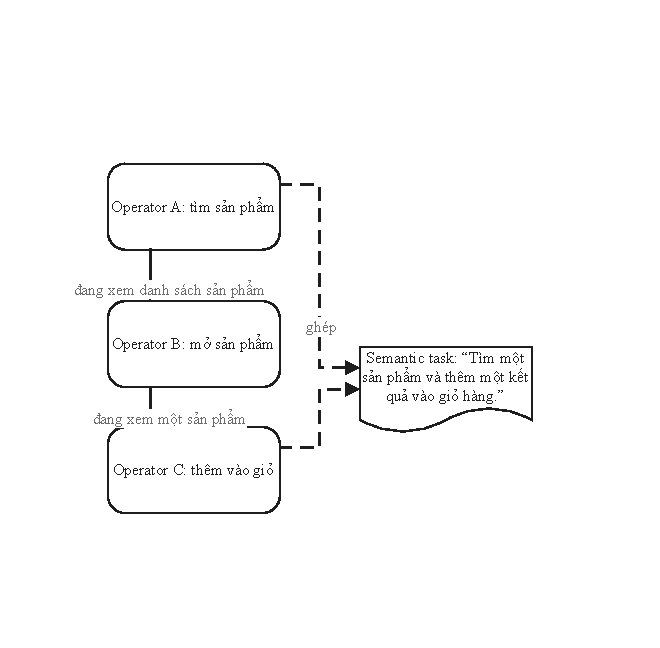
\includegraphics[width=0.78\textwidth]{Figures/fig_semantic.pdf}
\caption[Sinh semantic task bằng ghép chuỗi operator]{Sinh semantic task
bằng ghép chuỗi operator. Mỗi cạnh biểu diễn một trạng thái trung gian mà
effect của operator trước thỏa mãn precondition của operator kế tiếp. Các
chuỗi operator thu được tương ứng với những semantic task dài hạn, vượt ra
ngoài phạm vi của các task gắn với từng trang riêng lẻ.}
\label{fig:semantic}
\end{figure}

\subsection{Induction operator}

Sau khi một skill được thu nhận, thành phần \emph{inducer} sử dụng LLM để
suy ra \emph{precondition} và \emph{effect} của skill. Đầu vào gồm
\emph{SkillCard} cùng các quan sát ở đầu và cuối của một số trajectory đại
diện thuộc skill đó. Hai tập mệnh đề được sinh dưới dạng ngôn ngữ tự nhiên.

Prompt của bước này ràng buộc \emph{dạng} của mệnh đề chứ không chỉ nội dung,
và ràng buộc đó là điều kiện cần để việc ghép chuỗi về sau khả thi. Mỗi mệnh
đề phải mô tả một \emph{trạng thái trang} (``đang ở trang danh sách sản
phẩm'', ``trang giỏ hàng đang hiển thị'') chứ không phải sự hiện diện của một
phần tử đơn lẻ (``có một liên kết giỏ hàng trên trang''); phải có ít nhất một
precondition đặt tên cho trạng thái trang lúc vào và ít nhất một effect đặt
tên cho trạng thái trang lúc ra; và trạng thái lúc ra bắt buộc phải \emph{khác}
trạng thái lúc vào. Với một skill diễn ra gọn trong một trang, cách diễn đạt
được yêu cầu là giữ nguyên tên trang nhưng bổ nghĩa bằng điều mà skill vừa
thiết lập (``trang sửa sản phẩm \emph{đã có xác nhận lưu}''), tuyệt đối không
lùi về mức phần tử. Lý do của ràng buộc cuối này nằm ở chỗ chỉ một mệnh đề ở
mức trạng thái trang mới có cơ hội trùng với precondition của một skill khác;
lý do nó được viết thẳng vào prompt, thay vì được kỳ vọng, là kết quả của cổng
lọc ngay dưới đây (chi tiết ở Mục~\ref{sec:disc-operators}).

Nếu để LLM diễn đạt hoàn toàn tự do, các mệnh đề tương đương về ngữ nghĩa
thường được viết theo nhiều cách khác nhau, làm phân mảnh bộ từ vựng. Thực
nghiệm trên một lượt chạy cho thấy hiện tượng này xảy ra ngay cả khi sử dụng
sentence embedding để chuẩn hóa. Một cặp mệnh đề thực sự đồng nghĩa chỉ đạt
độ tương đồng 0{,}570, thấp hơn ngưỡng gộp 0{,}6, trong khi một cặp khác
nghĩa lại đạt 0{,}606; số liệu chi tiết được trình bày ở
Mục~\ref{sec:disc-operators}. Vì vậy, quá trình induction được thiết kế theo hướng \emph{vocabulary-aware}
(có nhận biết từ vựng đã dùng). Prompt cung cấp trước một tập các mệnh đề đã
có trong registry (sổ đăng ký mệnh đề, ưu tiên các mục được sử dụng nhiều và
mới nhất), đồng thời yêu cầu LLM tái sử dụng nguyên văn các mệnh đề tương
đương thay vì diễn đạt lại.

Operator sau khi sinh tiếp tục đi qua một bước kiểm tra
\emph{tautology} (mệnh đề hiển nhiên đúng). Các effect trùng hoàn toàn với
precondition sẽ bị loại bỏ

\[
\mathit{eff} \leftarrow \mathit{eff} \setminus \mathit{pre},
\]

và những skill không còn effect mới sau bước này sẽ không được nâng thành
operator. Mục đích của bước lọc là loại bỏ các operator không biểu diễn bất
kỳ thay đổi trạng thái nào, vì chúng không tạo ra cạnh mới trong đồ thị toán
tử và không thể tham gia vào quá trình ghép chuỗi.

Cổng lọc thứ hai kiểm tra một câu hỏi khác: mệnh đề vừa sinh ra có thực sự
đúng trên dữ liệu hay không. Khác với bước induction, vốn chỉ lấy hai
trajectory làm ngữ cảnh, bước này đối chiếu từng mệnh đề với trạng thái trang
trước và sau của \emph{mọi} thành viên trong cụm, rồi tính tỷ lệ số thành viên
mà mệnh đề đó thực sự đúng. Một effect được xác nhận trên dưới một nửa số
thành viên sẽ bị loại bỏ, và một operator không còn effect nào sau bước này sẽ
bị từ chối hoàn toàn. Ngưỡng này được đặt ở mức thận trọng, tương đương với
``chỉ loại những effect không đúng trên bất kỳ thành viên nào'', và nó có
nguyên nhân cụ thể: một lượt chạy trên Shopping Admin đã thu nhận một operator
với effect đạt độ chính xác 0{,}0, tức không đúng ở bất kỳ đâu, rồi vẫn lập kế
hoạch dựa trên nó.

Cần lưu ý rằng cổng này chỉ áp dụng cho effect. Các precondition cũng được
chấm điểm và ghi lại, nhưng không bao giờ bị loại bỏ, bởi việc gỡ đi một
precondition đáng ngờ sẽ khiến operator trở nên áp dụng được ở mọi nơi -- một
sai lầm nguy hiểm hơn nhiều so với việc quá thận trọng. Trong trường hợp cụm
không còn thành viên nào có dữ liệu trang để đối chiếu, cổng được bỏ qua thay
vì từ chối tất cả.

Một operator được đánh dấu là \emph{terminal} nếu ít nhất một trajectory thành
viên kết thúc tại trạng thái mục tiêu đã cấu hình, hoặc khi inducer xác định
skill đó tương ứng với việc hoàn thành mục tiêu.

\subsection{Chuẩn hóa mệnh đề}

Các mệnh đề sinh ra từ induction được chuẩn hóa thông qua
\emph{predicate registry} (sổ đăng ký mệnh đề). Thành phần này sử dụng cùng
cơ chế tính độ tương đồng cosine như thư viện skill, với ngưỡng mặc định
0{,}6 (Phụ lục~\ref{app:design-params}), nhưng không cho phép gộp các cụm đã
tồn tại, nhằm đảm bảo mỗi mã định danh sau khi cấp phát sẽ không thay đổi.

Đối với mỗi mệnh đề mới, hệ thống hoặc ánh xạ nó vào một cụm chuẩn hiện có và
kế thừa mã định danh của cụm đó, hoặc tạo một cụm mới nếu không tìm thấy
ứng viên phù hợp. Theo thời gian, registry xây dựng một tập predicate chung

\[
P=\{p_0,p_1,\ldots\},
\]

được chia sẻ bởi toàn bộ operator. Nhờ đó, việc so khớp giữa effect và
precondition chỉ còn là so sánh mã định danh thay vì so sánh trực tiếp chuỗi
văn bản, trong khi vẫn giữ được khả năng mở rộng bộ từ vựng thông qua LLM.

\subsection{Ghép chuỗi operator thành semantic task}

Đồ thị toán tử tạo một cạnh
$\omega_1 \rightarrow \omega_2$
nếu một effect của
$\omega_1$
khớp với một precondition của
$\omega_2$
sau bước chuẩn hóa. Trên đồ thị này, hệ thống sử dụng tìm kiếm theo chiều sâu
có chặn để liệt kê các đường đi đơn có độ dài từ hai trở lên. Các giới hạn về
độ dài chuỗi và số lượng đường đi được áp dụng nhằm tránh hiện tượng bùng nổ
tổ hợp khi đồ thị trở nên dày đặc.

Mỗi chuỗi operator thu được sẽ được chuyển thành một \emph{goal task} (tác vụ
mục tiêu). Nội
dung của task được tổng hợp từ mô tả của các skill trong chuỗi, còn điểm bắt
đầu lấy từ URL ghi nhận của operator đầu tiên. Chẳng hạn, nếu hệ thống đã
phát hiện hai skill ``tìm kiếm trong danh mục sản phẩm'' và ``thêm sản phẩm
đang hiển thị vào giỏ'', việc ghép hai operator tương ứng sẽ tạo ra một task
dạng \emph{``tìm một sản phẩm rồi thêm kết quả tìm được vào giỏ hàng''}.
Task này không được đề xuất từ bất kỳ trang riêng lẻ nào, mà được hình thành
từ quan hệ giữa các năng lực đã được kiểm chứng.

Các semantic task được thực thi theo chiến lược bảo thủ nhằm hạn chế lặp lại.
Trong mỗi lượt khám phá, mỗi chuỗi operator chỉ được thử tối đa một lần và
mỗi node chỉ sinh thêm một số lượng hữu hạn chuỗi mới. Thuật
toán~\ref{alg:semantic} mô tả toàn bộ quá trình này, từ việc liệt kê chuỗi
trên đồ thị toán tử cho tới cách chọn cơ chế kiểm chứng cho từng task.

\begin{algorithm}[H]
\caption{Sinh semantic task bằng ghép chuỗi operator}
\label{alg:semantic}
\begin{algorithmic}[1]
\Require đồ thị toán tử $G = (\Omega, E)$ với
$E = \{(\omega_1, \omega_2) : \mathit{eff}(\omega_1) \cap \mathit{pre}(\omega_2) \neq \emptyset\}$;
ngân sách $b$ chuỗi mới cho mỗi node; tập chuỗi đã thử trong lượt chạy $X$;
mục tiêu kết thúc $g_T$ (có thể không được cấu hình, ký hiệu $\bot$)
\Ensure danh sách semantic task kèm cơ chế kiểm chứng tương ứng
\State $P \gets \emptyset$
\For{mỗi $\omega \in \Omega$ theo thứ tự tất định}
  \State $\textsc{Dfs}([\omega])$
\EndFor
\State $T \gets \emptyset$
\For{mỗi chuỗi $p \in P$}
  \If{$|T| \ge b$} \textbf{break} \EndIf
  \If{$p \in X$} \textbf{continue} \Comment{mỗi chuỗi chỉ thử một lần trong một lượt chạy} \EndIf
  \State $X \gets X \cup \{p\}$
  \State $\mathit{instr} \gets$ URL khởi đầu ghi nhận của $p_1$, nối với mô tả các skill trong $p$ theo đúng thứ tự
  \If{$p_{|p|}$ được đánh dấu terminal \textbf{và} $g_T \neq \bot$}
    \State $\mathit{verify} \gets \textsc{Reached}(g_T)$ \Comment{kiểm chứng tất định}
  \Else
    \State $\mathit{verify} \gets$ kết luận của solver, judge kiểm tra lại ngay trong vòng lặp
  \EndIf
  \State $T \gets T \cup \{(\mathit{instr}, \mathit{verify}, |p|)\}$ \Comment{$|p|$ là độ khó}
\EndFor
\If{$T = \emptyset$ \textbf{và} $g_T \neq \bot$} \Comment{đồ thị còn quá thưa để ghép chuỗi}
  \State $p \gets \textsc{Plan}(G, \emptyset, g_T)$ \Comment{BFS tiến trên precondition/effect}
  \If{$p \neq \bot$}
    \State $T \gets \{(\text{tác vụ đạt mục tiêu kết thúc}, \textsc{Reached}(g_T), |p|)\}$
  \EndIf
\EndIf
\State \Return $T$
\Statex
\Function{Dfs}{$p$} \Comment{trả về \textbf{đúng} khi đã đủ số chuỗi cần liệt kê}
  \If{$|p| \ge \mathit{min\_len}$}
    \State $P \gets P \cup \{p\}$ \Comment{chuỗi con cũng là một task hợp lệ, ngắn hơn}
    \If{$|P| \ge \mathit{max\_paths}$} \State \Return \textbf{đúng} \EndIf
  \EndIf
  \If{$|p| \ge \mathit{max\_len}$} \State \Return \textbf{sai} \EndIf
  \For{mỗi $\omega'$ kế tiếp của $p_{|p|}$ theo thứ tự tất định, với $\omega' \notin p$}
    \If{$\textsc{Dfs}(p \text{ nối thêm } \omega')$} \State \Return \textbf{đúng} \EndIf
  \EndFor
  \State \Return \textbf{sai}
\EndFunction
\end{algorithmic}
\end{algorithm}

Việc đánh giá kết quả ưu tiên các tiêu chí tất định khi có thể. Nếu operator
cuối cùng là \emph{terminal} và website cung cấp điều kiện kết thúc có thể
kiểm tra bằng chương trình (chẳng hạn URL xác nhận đơn hàng), trạng thái
thành công sẽ được xác minh trực tiếp. Trong các trường hợp còn lại, episode
được đánh giá qua kết luận của solver và tiếp tục được một judge độc lập kiểm
tra lại \emph{ngay trong vòng lặp khám phá}: một phán quyết \textsc{Fail} sẽ
hạ episode xuống thất bại trước khi nó kịp đi vào bất kỳ khâu nào phía sau,
nên không episode nào được ghi nhận thành công chỉ dựa trên lời tự tuyên bố
của tác nhân (Mục~\ref{sec:method-data}, \ref{sec:disc-slm}).

Ở giai đoạn đầu khi đồ thị toán tử còn thưa và chưa hình thành được các chuỗi
hợp lệ, hệ thống tạm thời lập kế hoạch trực tiếp tới các trạng thái kết thúc
đã biết nếu có. Cơ chế này cho phép quá trình thu thập dữ liệu tiếp tục diễn
ra ngay cả trước khi đồ thị đủ phong phú để sinh semantic task.

\subsection{Seed năng lực website: nguồn mục tiêu từ trên xuống}
\label{sec:method-seed}

Cơ chế ghép chuỗi ở trên là một cơ chế \emph{từ dưới lên}: nó chỉ sinh được
task khi đồ thị toán tử đã có cạnh, mà cạnh lại chỉ hình thành khi hai
operator độc lập tình cờ phát biểu trùng một mệnh đề. Trong thực tế, điều
kiện này thưa hơn dự kiến rất nhiều (Mục~\ref{sec:disc-operators}), khiến
việc thu thập dữ liệu dài hạn bị treo vào tài sản khó xây dựng nhất của hệ
thống.

Vì vậy, hệ thống bổ sung một nguồn mục tiêu thứ hai, hoạt động \emph{từ trên
xuống} và không phụ thuộc đồ thị. Ở node đầu tiên của mỗi lượt khám phá,
thành phần \emph{site seeder} tóm tắt trang chủ thành một \emph{seed} gồm mô
tả website và một danh sách từ bốn tới tám năng lực mà website đó cho phép
người dùng thực hiện (chẳng hạn ``đặt hàng'', ``theo dõi trạng thái đơn
hàng'', ``quản lý sổ địa chỉ''). Mỗi năng lực trong seed trở thành một goal
task nhiều bước.

Prompt của seeder mang ba ràng buộc đáng chú ý, cả ba đều nhằm bảo đảm mục
tiêu sinh ra là thứ có thể chấm được. Thứ nhất, mỗi mục tiêu phải kết thúc ở
một trạng thái \emph{cụ thể và kiểm chứng được} từ trang kết quả, nên các hoạt
động mở như ``dạo xem danh mục điện tử'' bị cấm: đó là loại mục tiêu mà tuyên
bố hoàn thành gần như không tốn gì. Thứ hai, mọi giá trị đầu vào mà mục tiêu
cần phải hoặc được nêu thẳng trong mục tiêu, hoặc suy ra được từ trang (``sản
phẩm rẻ nhất'', ``đơn hàng gần nhất''); một mục tiêu để ngỏ giá trị cho tác
nhân tự nghĩ ra là mục tiêu mà tác nhân sẽ từ chối một cách hoàn toàn hợp lý.
Thứ ba, mọi năng lực phải bám vào những gì trang thật sự có, chứ không được
suy diễn ra các tính năng không nhìn thấy.

Ngân sách dành cho các mục tiêu này được phân bổ theo hai quy tắc. Một năng
lực có thể được thử lại tối đa ba lần trong một lượt chạy, mỗi lần từ một
\emph{loại} trang khác nhau (theo khuôn dạng URL), bởi cùng một mục tiêu theo
đuổi từ một điểm xuất phát khác thực sự là một quỹ đạo khác; ràng buộc theo
loại trang là thứ ngăn toàn bộ ngân sách bị tiêu hết trong vài node đầu tiên.
Ngược lại, một năng lực liên tiếp thất bại sẽ bị cho nghỉ sớm, và trường hợp
tác nhân tự tuyên bố bất khả thi thì bị cho nghỉ ngay lập tức: khi tác nhân đã
nhìn trang và kết luận rằng tính năng đó không tồn tại trên bản triển khai
này, kết luận ấy sẽ không đúng hơn ở trang thứ ba.

Seed đồng thời được đưa vào prompt của explorer làm ngữ cảnh, giúp các task
bậc thấp bám sát mục đích thật của website thay vì chỉ mô tả những gì trang
hiện tại hiển thị.

Hai nguồn này bổ trợ nhau và dùng chung ngân sách goal task của mỗi node:
ghép chuỗi cho ra các mục tiêu \emph{đã được kiểm chứng là khả thi} vì mọi
mắt xích đều là skill đã thu nhận, còn seed cho ra các mục tiêu \emph{đúng
mục đích của website} kể cả khi đồ thị còn trống. Tỷ trọng thực tế giữa hai
nguồn trong các lượt chạy thật được báo cáo ở Mục~\ref{sec:exp-data}.

So với các task được đề xuất độc lập trên từng trang, semantic task mang lại
hai lợi ích chính. Thứ nhất, chúng tạo ra các trajectory dài hơn, bao phủ
những chuỗi hành động nhiều bước thay vì chỉ các tương tác cục bộ. Thứ hai,
mỗi trajectory phản ánh việc phối hợp nhiều skill đã được kiểm chứng, từ đó
cung cấp các mẫu hành vi có cấu trúc phong phú hơn cho quá trình fine-tuning
mô hình ngôn ngữ nhỏ.

\section{Tinh lọc dữ liệu}
\label{sec:method-data}

Các episode thu được sau quá trình khám phá chưa thể sử dụng trực tiếp để
huấn luyện mô hình. Chúng tiếp tục trải qua ba giai đoạn xử lý nhằm kiểm soát
chất lượng và chuyển đổi thành tập dữ liệu fine-tuning, đồng thời duy trì
nguyên tắc \emph{prompt parity} trong toàn bộ pipeline
(Hình~\ref{fig:curation}).

\begin{figure}[htbp]
\centering
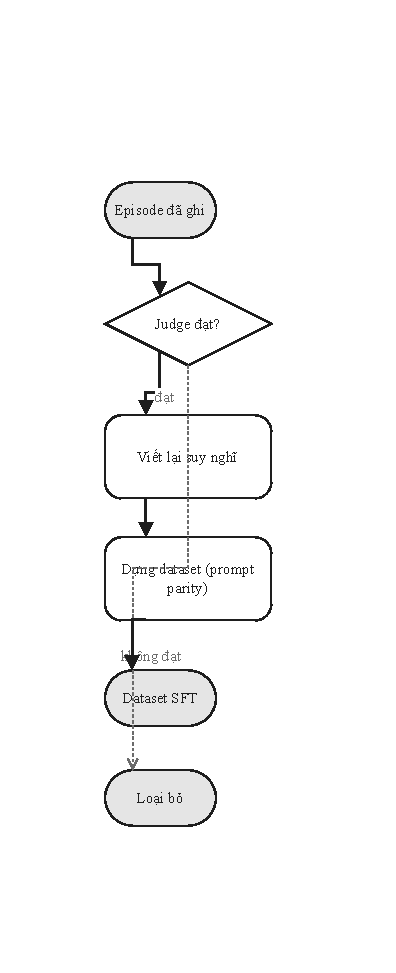
\includegraphics[width=0.50\textwidth]{Figures/fig_curation.pdf}
\caption[Pipeline tinh lọc dữ liệu]{Pipeline tinh lọc dữ liệu. Các episode
được một judge độc lập đánh giá lại, phần suy luận được chuẩn hóa, sau đó
được chuyển thành dữ liệu huấn luyện theo nguyên tắc prompt parity. Những
episode tự tuyên bố thành công nhưng không được judge xác nhận sẽ bị loại
khỏi tập dữ liệu.}
\label{fig:curation}
\end{figure}

\subsection{Chấm độc lập các thành công tự tuyên bố}

Một episode được solver kết luận là hoàn thành chưa đủ để xem là dữ liệu
đúng. Vì vậy, bước \emph{judge} sử dụng một LLM mạnh hơn để đánh giá lại tất
cả các episode tự tuyên bố thành công, theo cách tiếp cận dùng LLM làm bộ
chấm đã được kiểm chứng trong các nghiên cứu trước~\cite{zheng2023judge}.
Judge đối chiếu mục tiêu với trạng thái cuối của episode, bao gồm URL và nội
dung trang tại thời điểm kết thúc, rồi đưa ra một phán quyết độc lập. Những
phiên được xác minh bằng hàm kiểm tra tất định (\texttt{reached}) không đi qua
bước này, vì kết quả của chúng vốn đã đáng tin.

Điểm quan trọng là bước chấm này chạy \emph{ngay trong vòng lặp khám phá}, chứ
không phải sau khi lượt chạy kết thúc. Một phán quyết \textsc{Fail} hạ ngay
episode xuống thất bại \emph{trước khi} bất kỳ khâu nào phía sau nhìn thấy nó:
episode đó không được ghi là thành công, không đi vào khâu phát hiện kỹ năng,
và không được chọn cho lượt lấy mẫu không tiền tố. Vị trí của bước chấm là một
quyết định thiết kế có chủ đích: một phán quyết ngoại tuyến là phán quyết mà
lượt chạy \emph{không bao giờ hành động theo}, nên nó có thể sửa được tập dữ
liệu nhưng không sửa được những gì lượt chạy đã làm dựa trên kết luận sai.
Quyết định gọi judge cũng được đặt bên trong hàm giải một tác vụ thay vì ở các
nơi gọi hàm đó, để không một điểm gọi mới nào có thể vô tình bỏ qua nó. Hệ
thống vẫn giữ một kịch bản chấm ngoại tuyến độc lập, dùng chung prompt với bộ
chấm trực tuyến, để chấm lại các lượt chạy cũ thu thập trước khi cơ chế này
tồn tại.

Kết quả đánh giá của judge được lưu bổ sung bên cạnh kết luận ban đầu thay vì
ghi đè lên kết quả do solver tạo ra. Khi dựng dataset, hệ thống có thể lựa
chọn chỉ giữ lại các episode đã được judge xác nhận thành công, đồng thời
loại bỏ những episode chưa từng trải qua bước đánh giá này.

\subsection{Viết lại suy nghĩ (thought re-annotation)}

Chuỗi suy luận do solver sinh ra có chất lượng không đồng đều, trong khi đây
lại là tín hiệu mà mô hình fine-tune sẽ học theo. Do đó, mỗi bước suy luận
được viết lại theo một khuôn dạng thống nhất gồm bốn thành phần: (i) đánh giá
ngắn gọn về trạng thái hiện tại, (ii) phản tư nếu hành động trước đó không
đem lại tiến triển, (iii) \emph{subgoal} (mục tiêu con) của bước hiện tại và
(iv) ở bước kết thúc, một phép kiểm tra tường minh xem mục tiêu của task đã
được hoàn thành hay chưa.

Thành phần \emph{subgoal} được khôi phục bằng cách áp dụng lại chính thuật
toán phân đoạn trajectory sử dụng trong giai đoạn phát hiện skill. Quan trọng
hơn, thông tin này chỉ xuất hiện trong phần phản hồi của assistant
(\emph{assistant target}) và không được đưa vào prompt đầu vào. Thiết kế này
đảm bảo dữ liệu huấn luyện phản ánh đúng điều kiện suy luận thực tế, nơi mô
hình không được cung cấp trước subgoal của bước hiện tại.

\subsection{Dựng dataset với prompt parity}

Ở giai đoạn cuối, các episode được chuyển thành các mẫu instruction-tuning
(tinh chỉnh theo chỉ dẫn) theo nguyên tắc \emph{prompt parity}: cấu trúc
prompt sử dụng khi huấn luyện phải trùng khớp với prompt mà solver nhận được
trong quá trình suy luận.

Để đảm bảo tính nhất quán, system prompt được sử dụng trực tiếp từ solver thay
vì sao chép thủ công. Quan sát trang được cắt bằng đúng thủ tục tiền xử lý sử
dụng khi chạy agent, bao gồm cả các dấu hiệu cắt tường minh. Lịch sử tương
tác cũng được dựng theo đúng định dạng và chú thích kết quả mà agent quan sát
trong quá trình thực thi.

Những bước có hành động thực thi thất bại sẽ bị loại khỏi dữ liệu đích, vì
chúng là sai lầm chứ không phải cách khắc phục. Tuy nhiên chúng \emph{không}
bị xóa khỏi lịch sử của các bước sau: hành động đó đã thực sự xảy ra, và thông
báo lỗi mà nó sinh ra chính là thứ giải thích vì sao bước kế tiếp lại chọn một
hướng khác. Bỏ dòng lịch sử này đi thì mẫu huấn luyện của bước khắc phục sẽ
trông như được rút ra từ một trang chưa hề bị đụng tới, tức không còn khớp với
prompt mà mô hình thực sự nhìn thấy lúc suy luận.

Ngoài hai cổng đã nêu, khâu dựng dataset còn áp dụng ba bộ lọc ở mức episode.

\textbf{Cổng hành động hữu hiệu.} Một episode thuộc nhóm thay đổi trạng thái
hoặc điều hướng (\texttt{MOD}, \texttt{NAV}, \texttt{COMPOSITE}, hoặc một mục
tiêu ngữ nghĩa) sẽ bị loại nếu trong số các bước còn sống sau khi xuất ra
không có bất kỳ hành động nào thuộc nhóm có thể tác động lên trang. Nói cách
khác, một episode chỉ cuộn trang, di chuột hoặc chờ rồi tuyên bố hoàn thành là
một thành công giả, không phải một thành công ngắn. Cổng này bổ khuyết đúng
điểm mù của bộ chấm ngữ nghĩa: judge chỉ nhìn trạng thái cuối, mà trạng thái
cuối của một tác vụ ``sửa đổi'' không sửa gì thì trông hoàn toàn bình thường.
Nhóm \texttt{INFO} được miễn trừ, bởi trả lời ngay trên trang được đưa tới
chính là hình dạng đúng của nó.

\textbf{Loại bỏ báo cáo bất khả thi kiểu biện minh.} Chỉ những episode mà tác
nhân tự kết luận bất khả thi \emph{trong lúc} đang giải mới được giữ lại làm
mẫu huấn luyện. Những episode bị một chốt chặn dừng lại rồi mới phát ra
\texttt{report\_infeasible} ở lời gọi tổng kết đều bị loại, dựa trên lý do
dừng đã được lưu cùng episode (Mục~\ref{sec:method-solver}). Huấn luyện trên
nhóm sau là dạy mô hình bỏ cuộc, và hiệu ứng đó đo được: một tập dữ liệu chưa
lọc chứa 136 lần bỏ cuộc như vậy, chiếm 23\% số mẫu và tập trung vào đúng nhóm
tác vụ khó nhất, còn mô hình huấn luyện trên nó báo bất khả thi ở 39\% số tác
vụ Reddit khi đánh giá, đúng bằng tỷ lệ có trong dữ liệu.

\textbf{Loại bỏ hành động rời khỏi website.} Một hành động \texttt{goto} trỏ
tới một tên miền khác với trang hiện tại không bao giờ được dùng làm đích
huấn luyện. WebArena là tập hợp các bản sao tự triển khai của những website
thật, nên điều hướng sang chính website công khai mà bản sao đó mô phỏng sẽ
kết thúc phiên đánh giá với điểm 0. Khâu thu thập đã để lọt một hành động như
vậy, và mô hình sau fine-tune tái hiện đúng khuôn mẫu đó ở 10 trên 57 phiên
Reddit. Hành động này vẫn được giữ trong phần lịch sử, vì nó đã thực sự được
thực thi.

Mỗi mẫu dữ liệu đều mang theo mã trajectory, chỉ số bước và tổng số bước tương
ứng nhằm hỗ trợ quá trình gom lô theo trajectory. Cuối cùng, các mẫu được sắp
xếp theo mức độ khó tăng dần, với quy ước độ khó 1 cho quỹ đạo \texttt{LOCAL},
2 cho quỹ đạo \texttt{UNPREFIXED} và bằng độ dài chuỗi operator cho các mục
tiêu ngữ nghĩa, qua đó hình thành một curriculum cho quá trình fine-tuning
theo tinh thần của học theo chương trình (curriculum
learning)~\cite{bengio2009curriculum}.

\section{Fine-tune mô hình ngôn ngữ nhỏ}
\label{sec:method-sft}

Mô hình được sử dụng để fine-tune là Qwen3.5-9B~\cite{qwen2026qwen35}. Quá
trình huấn luyện áp dụng phương pháp
LoRA~\cite{hu2022lora} thông qua framework
LLaMA-Factory~\cite{zheng2024llamafactory}.

Việc chia tập huấn luyện và tập kiểm định được thực hiện theo đơn vị
\emph{tác vụ}, cụ thể là theo cặp (website, nội dung mục tiêu), chứ không theo
từng bước và cũng không theo từng quỹ đạo. Chia theo bước là sai hiển nhiên,
vì các bước trong cùng một episode quan hệ chặt với nhau. Nhưng chia theo quỹ
đạo cũng chưa đủ, và đây là điểm dễ bỏ sót: cơ chế lấy mẫu không tiền tố
(Mục~\ref{sec:method-unprefixed}) ghi lại mỗi tác vụ đã giải được \emph{hai}
lần, một lần từ chính trang của nó và một lần từ trang chủ, nên một mục tiêu
sở hữu hai quỹ đạo và một phép chia ở mức quỹ đạo sẽ đặt bản sao này vào tập
huấn luyện còn bản sao kia vào tập kiểm định. Đo trên chính tập dữ liệu của
khóa luận, cách chia đó làm rò rỉ 29 trên 56 quỹ đạo kiểm định, tương đương
một nửa số mẫu kiểm định: mô hình đã học đúng mục tiêu ấy, trên đúng website
ấy, tới đúng trang đích ấy. Hệ quả là giá trị \texttt{eval\_loss} trở nên lạc
quan và việc chọn checkpoint giữa các epoch dựa trên nó không còn đáng tin.

Hai xử lý phụ đi kèm phép chia. Thứ nhất, các bản lặp thừa bị loại bỏ: một mục
tiêu có đúng một quỹ đạo \texttt{LOCAL} và một quỹ đạo \texttt{UNPREFIXED} là
cặp đúng như thiết kế và được giữ nguyên, nhưng hai quỹ đạo \emph{cùng} mức độ
khó cho cùng một mục tiêu, vốn phát sinh khi một năng lực seed được đề xuất
lại ở node khác, chỉ giữ lại quỹ đạo dài nhất. Thứ hai, tập kiểm định được lấy
mẫu phân tầng theo từng website với cùng một tỷ lệ, thay vì lấy một lượt chung
trên toàn bộ dữ liệu; nếu không, website nào sở hữu các quỹ đạo dài nhất sẽ
chiếm phần lớn hạn mức kiểm định và \texttt{eval\_loss} sẽ chủ yếu phản ánh
riêng website đó.

Một điểm cần lưu ý khác là Qwen3.5-9B mặc định sinh ra các đoạn suy luận
tường minh (thinking), trong khi dữ liệu của khóa luận chỉ chứa các cặp
suy nghĩ--hành động đã được chuẩn hóa. Vì vậy, chat template được cấu hình
để vô hiệu hóa chế độ thinking trong cả quá trình huấn luyện lẫn suy luận,
đảm bảo định dạng đầu ra của mô hình nhất quán với dữ liệu huấn luyện.

Sau khi fine-tune, các trọng số LoRA được hợp nhất với mô hình gốc và triển
khai bằng vLLM~\cite{kwon2023vllm}. Cấu hình serving (phục vụ suy luận) tiếp
tục duy trì việc tắt chế độ thinking trên mọi yêu cầu. Nhờ đó, phân phối
prompt và đầu ra trong giai đoạn triển khai vẫn khớp với dữ liệu được sử dụng
khi huấn luyện, tương ứng với phía triển khai của nguyên tắc
\emph{prompt parity}.

\section{Ghi chú hiện thực hóa}
\label{sec:method-impl}

HSGE được hiện thực bằng Python. Bảng~\ref{tab:modules} trình bày sự tương
ứng giữa các giai đoạn của pipeline và các module trong hệ thống.

Một đặc điểm của kiến trúc là mỗi vai trò sử dụng LLM (site seeder, explorer,
solver, solver riêng cho tác vụ ngữ nghĩa, bộ lập kế hoạch subgoal, bộ cắt
đoạn, bộ trừu tượng hóa, bộ kiểm chứng, inducer, judge và bộ viết lại suy
luận) đều có thể cấu hình mô hình độc lập. Nhờ đó, các thành phần được gọi
thường xuyên có thể sử dụng những mô hình chi phí thấp hơn, trong khi các mô
hình mạnh hơn được dành cho những bước yêu cầu chất lượng cao như giải tác vụ
ngữ nghĩa, operator induction và judge. Hai vai trò tương tác trực tiếp với
trang, tức explorer và solver, còn có thể được bật chế độ thị giác: khi đó
prompt được đính kèm ảnh chụp màn hình, tùy chọn phủ thêm lớp đánh dấu
Set-of-Marks vẽ khung bao quanh các phần tử theo đúng mã định danh xuất hiện
trong cây trợ năng. Vì một lời gọi có đính ảnh đôi khi bị phía nhà cung cấp
trả về rỗng, cả hai vai trò đều thử lại một lần ở chế độ thuần văn bản trước
khi chấp nhận thất bại.

Việc đăng nhập vào các website có xác thực được thực hiện một lần và lưu lại
trạng thái phiên; các lượt chạy sau nạp lại trạng thái đã lưu và bắt đầu trong
tình trạng đã đăng nhập, thay vì lặp lại luồng đăng nhập. Đây cũng là lý do
mọi tác vụ liên quan tới tài khoản đều bị cấm ở khâu đề xuất
(Mục~\ref{sec:method-lowlevel}): tài khoản là tài nguyên dùng chung giữa các
lượt chạy, và một thao tác đăng xuất hay đổi mật khẩu có thể khóa toàn bộ các
lượt chạy sau ra ngoài.

Toàn bộ pipeline cũng được thiết kế theo hướng tách biệt giữa thuật toán và
backend (lớp thực thi bên dưới). Hệ thống hỗ trợ cả backend thật và các
backend mô phỏng tất định (LLM theo kịch bản, embedding giả lập và website mô
phỏng), trong đó backend thật chỉ là một hiện thực khác của cùng giao diện. Thiết kế này
cho phép kiểm thử đơn vị các thành phần cốt lõi bằng các điều kiện kiểm tra
xác định, đồng thời giảm sự phụ thuộc vào chi phí API cũng như trạng thái
hoạt động của website trong quá trình phát triển.

Để hỗ trợ khả năng khôi phục sau khi gián đoạn, các sản phẩm trung gian như
skill, operator, đồ thị toán tử, kết quả khám phá của từng node và nhật ký sự
kiện đều được lưu sau mỗi node khám phá. Ngoài các sản phẩm ở dạng đọc được,
hệ thống còn ghi một điểm kiểm tra (checkpoint) nhị phân chứa toàn bộ trạng
thái vòng lặp, gồm hàng đợi frontier, tập đã thăm, các bộ đếm và toàn bộ đối
tượng của khâu phát hiện. Điểm kiểm tra được ghi theo cơ chế thay thế nguyên
tử sau mỗi node, nên một lần dừng đột ngột chỉ mất đúng node đang xử lý dở, và
lượt chạy có thể nối tiếp từ đúng chỗ đã dừng thay vì bắt đầu lại. Các đối
tượng backend (khách LLM, bộ nhúng) không tuần tự hóa được nên được tháo ra
trước khi ghi và gắn lại sau khi nạp.

Ngoài ra, mọi thao tác trình duyệt trong vòng lặp đều được thiết kế theo hướng
hỏng mềm (fail-soft): một node không tải được sẽ được ghi log, ghi nhận kèm
lỗi rồi bỏ qua, thay vì làm dừng cả lượt chạy nhiều giờ. Ngược lại, một ngoại
lệ thật sự bất ngờ ở bất kỳ nơi nào khác vẫn được để cho lan lên và làm dừng
lượt chạy một cách ồn ào, sau khi đã ghi lại trạng thái lỗi.

\begin{table}[H]
\centering
\caption[Các giai đoạn pipeline và module hiện thực]{Các giai đoạn pipeline
và module hiện thực tương ứng.}
\label{tab:modules}
\begin{tabular}{@{}L{5.2cm} L{8.0cm}@{}}
\toprule
\textbf{Giai đoạn} & \textbf{Module} \\
\midrule
Vòng khám phá, frontier &
\texttt{webarena/runtime},
\texttt{webarena/browser} \\

Đề xuất và giải task &
\texttt{webarena/agents} \\

URL độc lập máy chủ &
\texttt{webarena/urls} \\

Đăng nhập và phiên đã lưu &
\texttt{webarena/auth} \\

Cắt đoạn &
\texttt{segmentation},
\texttt{discovery} \\

Gom cụm, thư viện skill &
\texttt{clustering},
\texttt{abstraction},
\texttt{library} \\

Operator và lập kế hoạch &
\texttt{operators},
\texttt{operator\_induction},
\texttt{predicate\_registry} \\

Chấm lại episode (trực tuyến và ngoại tuyến) &
\texttt{webarena/verify},
\texttt{judge\_episodes} \\

Tinh lọc dữ liệu &
\texttt{reannotate\_thoughts},
\texttt{build\_sft\_dataset} \\

Chia train/val, gộp nhiều website &
\texttt{training/prepare\_dataset},
\texttt{training/merge\_datasets} \\

Huấn luyện và serving &
cấu hình LLaMA-Factory, script vLLM \\
\bottomrule
\end{tabular}
\end{table}

\vspace{1em}
\noindent
Sau khi trình bày toàn bộ phương pháp, chương tiếp theo đánh giá hiệu quả của
pipeline trên môi trường WebArena. Nội dung thực nghiệm tập trung vào hai câu
hỏi: pipeline thu thập được bao nhiêu dữ liệu huấn luyện từ website thực tế,
và việc fine-tune trên tập dữ liệu này có cải thiện khả năng thực hiện task
của mô hình trên benchmark WebArena hay không.


\chapter{Thực nghiệm}
\label{ch:experiments}

Chương này (1) mô tả môi trường thực nghiệm và quy trình đánh giá, (2) báo
cáo kết quả thu thập dữ liệu, (3) báo cáo kết quả fine-tuning, (4) trình
bày đánh giá chính trên bộ task chính thức của bốn website WebArena, và
(5) phân tích kết quả.

% GHI CHÚ: chương này dựng khung trước và sẽ được bổ sung khi các thực
% nghiệm còn lại hoàn tất (các mốc [BỔ SUNG]). Số liệu hiện có lấy từ đợt
% đánh giá GitLab ngày 15/07/2026.

\section{Môi trường thực nghiệm}
\label{sec:exp-setup}
% TODO: các instance WebArena tự triển khai; vast.ai A100-80GB cho huấn
% luyện và serving; bảng cấu hình LLM theo vai trò; tham số run; đánh giá
% qua BrowserGym scored environments + bộ chấm chính thức, phát lại hành
% động trả lời cuối.
\textit{[Sẽ viết — xem dàn ý 07, mục 4.1.]}

\section{Kết quả thu thập dữ liệu}
\label{sec:exp-data}
% TODO: thống kê từng run (node, task đề xuất/giải được/bất khả thi,
% skill, operator, chuỗi); dataset cuối: 370 mẫu (352 train / 18 val);
% 1-2 ví dụ tiêu biểu về skill và semantic task.
\textit{[Sẽ viết — xem dàn ý 07, mục 4.2.]}

\section{Kết quả fine-tuning}
\label{sec:exp-sft}
% TODO: đường loss (train 0.32 / eval 0.24), bảng thời gian và chi phí.
\textit{[Sẽ viết — xem dàn ý 07, mục 4.3.]}

\section{Đánh giá chính trên WebArena}
\label{sec:exp-main}
% Đánh giá trên BỐN website: Shopping, Shopping Admin, GitLab, Reddit.
% Hiện có: GitLab — mô hình gốc 10/180 (5,56%) vs fine-tune 12/180 (6,67%).
% Trình bày là tín hiệu định hướng (mỗi task chạy 1 lần) cho tới khi có 4.5.
% [BỔ SUNG] kết quả Shopping / Shopping Admin / Reddit + bảng theo website.
\textit{[Sẽ viết — xem dàn ý 07, mục 4.4.]}

\section{Lặp lại thống kê}
\label{sec:exp-stats}
% [BỔ SUNG] chạy lặp >=3-5 lần (hoặc nhiều seed) mỗi mô hình -> mean +/- SD,
% 95% CI, kiểm định phi tham số. Ưu tiên số 1.
\textit{[Dự kiến — xem dàn ý 07, mục 4.5.]}

\section{Nghiên cứu ablation}
\label{sec:exp-ablation}
% [BỔ SUNG] (a) dữ liệu khám phá theo graph vs khám phá phẳng cùng ngân
% sách; (b) có/không judge; (c) có/không viết lại suy nghĩ; (d) phân tích
% liên-website từ kết quả 4 website.
\textit{[Dự kiến — xem dàn ý 07, mục 4.6.]}

\section{Phân tích}
\label{sec:exp-analysis}
% TODO: phân rã theo loại task, ví dụ thành công/thất bại định tính,
% phân loại lỗi (nối sang Chương 5).
\textit{[Sẽ viết — xem dàn ý 07, mục 4.7.]}


\chapter{Thảo luận}
\label{ch:discussion}

Chương này (1) diễn giải các kết quả thực nghiệm của
Chương~\ref{ch:experiments}, sau đó chưng cất kinh nghiệm kỹ thuật thu được
khi xây dựng và vận hành pipeline thành các bài học về (2) khám phá website
thật, (3) dựng chốt chặn cấu trúc cho LLM agent thay vì chỉ nhắc nhở qua
prompt, (4) induction các operator chất lượng cao, và (5) huấn luyện và
serving mô hình ngôn ngữ nhỏ, trước khi (6) tổng hợp thành các best
practice và (7) bàn về các nguy cơ đối với tính hợp lệ. Mỗi bài học theo
cùng một khuôn: một vấn đề gặp thật trong các run của chúng tôi, chẩn đoán,
cách khắc phục, và nguyên tắc tổng quát rút ra. Chi tiết đầy đủ các sự cố
được tập hợp ở Phụ lục~\ref{app:runs}.

\section{Diễn giải kết quả}
\label{sec:disc-results}

% TODO: làm mới mục này khi có kết quả ba website còn lại và các lần lặp
% thống kê (Mục 4.5-4.6).

Con số nổi bật nhất đến nay, cải thiện từ 5{,}56\% lên 6{,}67\% tỷ lệ
hoàn thành trên bộ task GitLab chính thức, cần được đọc thận trọng thay
vì đắc thắng. Về tuyệt đối, mức tăng là nhỏ, và với mỗi task chỉ chạy một
lần, nó phải được coi là tín hiệu định hướng cho tới khi các lần chạy lặp
của Mục~\ref{sec:exp-stats} hoàn tất. Điều khiến tín hiệu này đáng chú ý là
hồ sơ chi phí của nó: nó thu được từ vỏn vẹn 352 mẫu huấn luyện, thu thập
tự động từ một website không có nhãn, và bản thân việc fine-tune mất chưa
đầy nửa giờ trên một GPU. Nói cách khác, pipeline đã dịch chuyển một mô
hình nhỏ đúng hướng với lượng dữ liệu nhỏ đáng kinh ngạc; câu hỏi mở là xu
hướng này kéo dài tới đâu khi thu thập dữ liệu mở rộng quy mô, điều mà
kết quả liên-website ở Mục~\ref{sec:exp-main} sẽ bắt đầu trả lời.

Ba yếu tố nhiều khả năng đang chặn mức tăng hiện tại. Thứ nhất, cỡ dữ
liệu: 352 mẫu thấp hơn các kho fine-tune agent điển hình hai đến ba bậc,
nên mô hình chỉ thấy mỗi khuôn tương tác vài lần. Thứ hai, độ phủ: dữ liệu
huấn luyện thu từ một phần website, trong khi benchmark rút task từ toàn
site. Thứ ba, chính mô hình gốc: một mô hình 9B tham số fine-tune thuần
giám sát không thể được kỳ vọng khôi phục các năng lực (lập kế hoạch dài
hạn, tự sửa lỗi) mà trajectory chỉ minh họa thưa thớt. Không yếu tố nào
trong ba điều trên quy lỗi cho thiết kế pipeline; cả ba đều chỉ về khối
lượng và độ phủ dữ liệu như ràng buộc trói buộc, đúng ràng buộc mà
pipeline được sinh ra để nới lỏng.

Quan trọng không kém là những gì lần chạy đầu--cuối đã \emph{chứng minh}:
mọi công đoạn (khám phá, phát hiện, ghép chuỗi operator, tinh lọc, huấn
luyện, serving, đánh giá chính thức) đều chạy trên website thật không
cần can thiệp tay, và các cổng chất lượng đã chặn được những dữ liệu lẽ ra
sẽ làm bẩn huấn luyện (Mục~\ref{sec:disc-slm}). Phần còn lại của chương kể
lại cái giá để câu vừa rồi đúng.

\section{Bài học khi khám phá website thật}
\label{sec:disc-exploration}

\subsection{Frontier cạn kiệt}

\textbf{Vấn đề.} Một run khám phá sớm trên website kiểu Reddit khựng lại ở
57 trên ngân sách 500 node: frontier đơn giản là cạn.
\textbf{Chẩn đoán.} Khi đó frontier chỉ lớn lên từ các URL solver tình cờ
điều hướng tới. Trang nào mà mọi task đề xuất đều thuộc dạng tra cứu thì
không sinh điều hướng nào, nên nguyên vùng website không bao giờ vào hàng
đợi; khám phá bị bắt làm con tin bởi việc explorer tình cờ đề xuất gì.
\textbf{Khắc phục.} Bổ sung khai thác hyperlink làm tầng frontier thứ hai,
kèm URL template và trần mỗi-template để trang gần trùng không tràn hàng
đợi (Mục~\ref{sec:method-frontier}).
\textbf{Bài học.} Trên website thật, \emph{khả năng chạm tới không được
phụ thuộc hành vi giải task}. Tín hiệu cấu trúc (link) và tín hiệu hành vi
(điều hướng) là hai nguồn frontier bổ trợ, và nguồn cấu trúc cần kiểm soát
đa dạng tường minh vì nó đến theo lô.

\subsection{Đề xuất task bị suy sụp}

\textbf{Vấn đề.} Trong một run thực tế, 46\% tổng số task đề xuất gần như
trùng nhau giữa các trang; các biến thể của ``vào trang Diễn đàn'' được
đề xuất lại ở hầu như mọi node.
\textbf{Chẩn đoán.} Mọi trang của một website chung menu điều hướng toàn
cục, còn một explorer bị prompt theo từng trang thì không nhớ mình đã đề
xuất gì ở nơi khác.
\textbf{Khắc phục.} Explorer giờ tồn tại suốt run: các đề xuất gần đây được
đưa ngược vào prompt làm ngữ cảnh phủ định, các bản gần trùng bị loại thêm
ở mức mã (Mục~\ref{sec:method-lowlevel}).
\textbf{Bài học.} Sự đa dạng của task sinh ra là thuộc tính \emph{cấp
run}, không phải cấp trang; nó phải được thi hành bằng trạng thái sống lâu
hơn bất kỳ lời gọi LLM đơn lẻ nào.

\subsection{Trang không đáng tin}

\textbf{Vấn đề.} Một trang chậm duy nhất, timeout điều hướng trên một
URL khai thác được, làm sập nguyên một run khám phá nhiều giờ.
\textbf{Chẩn đoán.} Các thao tác trình duyệt được tin tưởng ngầm định; một
ngoại lệ không bắt ở bất kỳ đâu trong xử lý node lan thẳng lên đỉnh.
\textbf{Khắc phục.} Mọi thao tác trình duyệt giờ đều fail-soft: node không
mở được thì ghi log, lưu kèm lỗi, rồi bỏ qua; còn ngoại lệ thật sự bất ngờ
vẫn làm run dừng có tiếng động. Sản phẩm trung gian được lưu sau mỗi node,
nên run bị ngắt vẫn để lại bản chụp nhất quán, nối lại được.
\textbf{Bài học.} Hãy coi mọi tương tác với website thật là thao tác
\emph{rồi sẽ} thất bại, và quyết định cho từng thao tác xem thất bại có
sống sót được không; làm cho tiến độ của run bền vững ở mức hạt mịn nhất
ngân sách cho phép.

\subsection{Trạng thái dùng chung, có thể bị sửa}

\textbf{Vấn đề.} Website benchmark là tài nguyên dùng chung và có trạng
thái: một agent bất cẩn có thể làm bẩn (hoặc phá hủy) môi trường mà
các run khác phụ thuộc.
\textbf{Khắc phục.} Ba lớp kỷ luật. Lớp thứ nhất là chế độ read-only, loại
các task thay đổi trạng thái theo nguyên tắc fail-closed: task không phân
loại được thì bị coi là có thay đổi. Lớp thứ hai là một luật cứng cấm các
task phá hoại cấp tài khoản bất kể chế độ. Lớp thứ ba áp dụng khi đánh giá
trên instance sống dùng chung: task benchmark được phân loại theo ý định
thành hai tập read-only và read-write, để hai máy có thể quét cùng website đồng
thời mà không giẫm chân nhau (Mục~\ref{sec:disc-slm}).
\textbf{Bài học.} Trên hạ tầng dùng chung, an toàn phải
\emph{fail-closed}: gánh nặng chứng minh thuộc về việc một task vô hại,
chứ không phải việc nó có hại.

\section{Chốt chặn cấu trúc thay vì nhắc nhở qua prompt}
\label{sec:disc-guardrails}

Một chủ đề lặp lại trong các run của chúng tôi: bảo mô hình cư xử đúng
không đồng nghĩa hệ thống cư xử đúng. Các sự cố dưới đây đều khởi đầu là
một quy ước mức prompt bị mô hình thật lặng lẽ vi phạm, và đều kết thúc
bằng một cơ chế cấu trúc không phụ thuộc sự vâng lời của mô hình.

\subsection{Quy ước gắn thẻ không sống sót khi gặp mô hình thật}

\textbf{Vấn đề.} Đề xuất task ban đầu được phân loại bằng thẻ
\texttt{[INFO]}\slash\texttt{[NAV]}\slash\texttt{[MOD]} đặt đầu câu mà
explorer được chỉ thị phải ghi. Trong một run thực tế, 89\% đề xuất không mang thẻ nào.
\textbf{Chẩn đoán.} Xu hướng tự nhiên của mô hình là trả phân loại trong
một trường \texttt{type} có cấu trúc (thứ mà parser vứt bỏ) thay vì
một cặp ngoặc trong chuỗi. Tệ hơn, phép kiểm tra an toàn cho task thay đổi
trạng thái là so khớp chuỗi ký tự trên \texttt{[MOD]}, nên một task phá
hoại không gắn thẻ sẽ lọt qua êm ái.
\textbf{Khắc phục.} Đề xuất giờ được yêu cầu và phân tích như đối tượng có
cấu trúc với trường phân loại tường minh; thứ gì không phân loại được gắn
\texttt{UNKNOWN} và bị loại trong chế độ read-only.
\textbf{Bài học.} Hãy xin mô hình \emph{cấu trúc}, đừng xin quy ước định
dạng bên trong văn bản tự do, và tuyệt đối đừng xây phép kiểm tra an
toàn trên một quy ước mà mô hình có thể không theo.

\subsection{Vòng kẹt, qua hai lần lặp}

\textbf{Vấn đề.} Solver đốt trọn ngân sách bước để lặp một hành động rõ
ràng không có tác dụng; trong một episode ghi lại được, nó click cùng
một phần tử trơ suốt cả mười lăm bước.
\textbf{Chẩn đoán và khắc phục lần một.} Chúng tôi thêm một cảnh báo, tiêm
vào prompt sau hai hành động liên tiếp không hiệu ứng trên cùng đích. Run
thật kế tiếp bác bỏ cách sửa này: mô hình tiếp tục click dù cảnh báo hiện
diện từ lời gọi thứ ba trở đi. Nó cũng lộ ra một điểm tinh vi: mô hình
đôi khi thử lại một dropdown bị kẹt bằng các đối số trông-khác-nhưng-sai-
như-nhau, nên so trùng nguyên văn chuỗi hành động sẽ bỏ lọt vòng kẹt.
\textbf{Khắc phục lần hai.} Bộ phát hiện kẹt giờ khóa theo \emph{đích} bị
tác động và theo việc quan sát có đổi không; sau một số lần lặp không tiến
triển có giới hạn, episode bị chấm dứt thẳng, không tốn thêm lời gọi LLM
nào. Yêu cầu ``không thay đổi quan sát được'' giữ chốt chặn khỏi kích hoạt
nhầm trên các chuỗi hợp lệ tái dùng một phần tử qua các trang thay đổi.
\textbf{Bài học.} Cảnh báo trong prompt là một lời gợi ý; ngân sách là một
cơ chế. Khi mô hình chứng minh nó phớt lờ gợi ý, hãy leo thang thành cơ chế
và kiểm chứng bước leo thang trên hành vi thật, không phải trên hành vi
mà prompt yêu cầu.

\subsection{Các sự cố nhỏ hơn, cùng một khuôn}

Ba sự cố nữa theo đúng khuôn trên và nhận cùng kiểu sửa. Task tra cứu do
explorer đề xuất đôi khi chứa sẵn đáp án (``tìm bài đăng có tiêu đề X''),
thứ solver ``giải'' được mà không học gì; khâu sinh giờ có chỉ thị chống
điều đó và các task lộ đáp án bị lọc. Lời gọi có đính kèm ảnh thỉnh thoảng
trả về rỗng (từ chối phía thượng nguồn); agent thử lại một lần ở chế độ
thuần văn bản thay vì hỏng cả bước. Và các episode cạn ngân sách trước đây
kết thúc bằng một thất bại câm lặng. Giờ chúng nhận một lời gọi wrap-up
cuối, thuần văn bản, mà đầu ra hợp lệ \emph{duy nhất} là tuyên bố hoàn
thành hoặc báo cáo bất khả thi, biến một lần hết giờ im lặng thành một
kết cục có nhãn mà dataset dùng được.

\section{Bài học từ induction operator}
\label{sec:disc-operators}

Cơ chế semantic task của Mục~\ref{sec:method-semantic} chỉ tốt ngang các
operator nó ghép. Hai chế độ hỏng lộ ra khi chúng tôi kiểm toán các
operator sinh trong một run thực tế sớm, và cả hai đều dẫn tới các cổng
chặn cấu trúc thay vì chỉnh prompt.

\subsection{Operator tautology}

\textbf{Vấn đề.} Ba trong bốn operator sinh ra trong run đó có tập effect
trùng hệt tập precondition.
\textbf{Chẩn đoán.} Khi được yêu cầu mô tả precondition và effect của một
skill, LLM thấy dễ nhất là nhắc lại bối cảnh: ``đang ở danh sách issue''
trước, ``đang ở danh sách issue'' sau. Operator như vậy không mã hóa thay
đổi trạng thái nào, nên không bao giờ đứng giữa chuỗi và không dẫn tới đâu
mới; nếu bỏ mặc, tautology sẽ lấp đầy đồ thị toán tử bằng các node chết.
\textbf{Khắc phục.} Cổng chặn tautology: effect nào lặp lại precondition bị
bỏ, và skill không còn effect mới bị từ chối nâng cấp, có ghi log lý do.
\textbf{Bài học.} Với các sản phẩm ký hiệu do LLM viết, \emph{hãy định
nghĩa tính hợp lệ theo lý thuyết tập hợp và thi hành nó bằng mã}; đừng
trông cậy prompt cấm được các câu trả lời thoái hóa.

\subsection{Mệnh đề đồng nghĩa mà embedding không gộp nổi}

\textbf{Vấn đề.} Ghép chuỗi đòi hỏi effect của operator này khớp
precondition của operator kia, nhưng các operator induction độc lập diễn
đạt cùng một điều kiện theo những cách khác nhau.
\textbf{Chẩn đoán.} Chúng tôi đo độ tương đồng embedding của các cặp mệnh
đề trong cùng run: một cặp diễn đạt tương đương thật chấm 0{,}570, 
\emph{dưới} ngưỡng chuẩn hóa 0{,}6, trong khi một cặp khác nghĩa chấm
0{,}606, trên ngưỡng. Không ngưỡng nào tách được hai trường hợp; chuẩn hóa
thuần hình học không thể khôi phục một bộ từ vựng chung sau khi sự đã rồi.
\textbf{Khắc phục.} Phòng thay vì chữa: induction nhận biết từ vựng. Prompt
trình các nhãn mệnh đề sẵn có của registry kèm chỉ thị tái sử dụng nguyên
văn mệnh đề tương đương, để việc thống nhất diễn ra lúc \emph{viết} (nơi
mô hình có đủ ngữ cảnh) thay vì lúc so embedding, nơi chỉ còn bề mặt câu
chữ.
\textbf{Bài học.} Khi hai đầu ra LLM về sau phải \emph{khớp} nhau, hãy chia
sẻ bộ từ vựng ngay lúc sinh; đừng ủy thác việc thống nhất ngữ nghĩa cho một
thước đo tương đồng.

\section{Cạm bẫy khi huấn luyện và serving SLM}
\label{sec:disc-slm}

\subsection{Chat template là một phần của mô hình}

Họ mô hình đích mặc định phát các đoạn suy nghĩ tường minh, trong khi đích
huấn luyện của chúng tôi là các cặp thought-action trần. Chat template
đúng (đã tắt thinking) phải được tìm từ registry template của framework
huấn luyện thay vì đoán theo tài liệu, và cùng thiết lập đó phải được áp
lại, trên từng request, lúc serving. Lệch ở bất kỳ phía nào là âm thầm huấn
luyện hoặc đánh giá một phân phối khác với dự định. Điểm tổng quát:
\emph{template và cấu hình giải mã là một phần của sản phẩm mô hình}, và
cấu hình lúc huấn luyện với lúc serving phải được ghim cùng nhau.

\subsection{Lỗi prompt-fidelity}

Thất bại nhiều bài học nhất của khâu huấn luyện không sinh ra lỗi nào. Một
bài kiểm nhanh sau huấn luyện, viết bằng một prompt \emph{xấp xỉ} prompt
của solver, khiến mô hình fine-tune phát ra mô tả bằng lời thay vì hành
động thực thi được, trông y hệt một lần fine-tune hỏng. Mô hình không
sao cả; prompt kiểm thử mới là thứ không trung thực. Kiểm lại bằng prompt
sản xuất (import từ solver, không gõ lại) cho hành động đúng. Sự cố
này là lý do prompt parity (Mục~\ref{sec:method-data}) được thi hành bằng
cách \emph{import} system prompt thật và các hàm phụ trợ của nó vào trình
dựng dataset lẫn bộ đánh giá, không bao giờ bằng cách chép tay. Mọi bài
kiểm một agent fine-tune chỉ đáng tin ngang độ trung thực của prompt kiểm
so với sản xuất.

\subsection{Cách ly phụ thuộc}

Hỗ trợ một kiến trúc mô hình mới phát hành đòi hỏi bản phát triển của thư
viện mô hình hóa, xung đột với yêu cầu ghim phiên bản của engine serving.
Ba môi trường cách ly (huấn luyện, serving, đánh giá) giải quyết điều
mà không môi trường đơn nào thỏa mãn nổi. Tầm thường, nhưng nó biến một
xung đột phiên bản vô phương thành một bước cài đặt thường quy.

\subsection{Agent tự chấm bài mình}

Bước judge được đưa vào vì thành công do solver tự tuyên bố không thể được xem là bằng chứng đáng tin cậy về việc hoàn thành tác vụ. Khi solver trả lời rằng tác vụ đã “hoàn tất”, nó đồng thời tự đánh giá kết quả của chính mình. Vì vậy, các episode được tuyên bố thành công cần được đánh giá lại dựa trên trạng thái cuối thực tế.

Cơ chế này giúp phát hiện những trường hợp solver tự kết luận sai rằng tác vụ đã thành công trước khi các trajectory tương ứng được đưa vào tập dữ liệu huấn luyện. Trong chế độ nghiêm ngặt, trình dựng dataset mặc định loại bỏ mọi trajectory được tuyên bố thành công nhưng chưa qua judge, thay vì mặc nhiên chấp nhận chúng.

Theo nguyên tắc P1, \emph{dữ liệu chưa được kiểm chứng không phải là dữ liệu trung tính; đó là một khoản nợ chất lượng có thể bị khuếch đại trong quá trình huấn luyện}.

\subsection{Đánh giá an toàn trên website sống dùng chung}

Chạy hai lượt đánh giá (gốc và fine-tune) trên một instance website sống
bình thường sẽ phải xếp hàng trọn một ngày làm việc. Phân loại task
benchmark theo ý định thành hai tập read-only và read-write cho phép máy thứ hai
đánh giá tập read-only song song với lượt quét không hạn chế của máy thứ
nhất. Bản thân việc phân loại chứa hai cái bẫy đáng ghi lại: va chạm cụm
danh từ (``merge request'' chứa động từ chỉ về mặt cú pháp; ``report bugs''
không gọi tên hành động báo cáo mà regex chờ đợi) và việc chèn từ đánh bại
các mẫu so cụm ngây thơ (``open \emph{a new} issue''). Chi phí truyền tải
cũng đáng kể: chuyển adapter LoRA 1{,}7\,GB rồi gộp lại tại chỗ thắng việc
chuyển checkpoint đã gộp 18\,GB.

\section{Best practice}
\label{sec:disc-practices}

Bảng~\ref{tab:practices} cô đọng các bài học của chương thành những thực
hành chúng tôi sẽ áp dụng từ ngày đầu của một dự án tương tự.

\begin{table}[H]
\centering
\caption[Các best practice đã chưng cất]{Các best practice cho pipeline
thu thập dữ liệu bằng LLM agent trên website thật.}
\label{tab:practices}
\small
\begin{tabular}{@{}L{4.4cm} L{8.8cm}@{}}
\toprule
\textbf{Thực hành} & \textbf{Lý do (mục)} \\
\midrule
Kiểm chứng rồi mới thu nhận & Skill, operator, thành công đều là khoản nợ
cho tới khi được kiểm độc lập (\ref{sec:disc-slm}, \ref{sec:disc-operators}) \\
Prompt parity bằng import & Dữ liệu huấn luyện, agent thật, bộ đánh giá
dùng chung một nguồn prompt; chép tay sẽ trôi dạt (\ref{sec:disc-slm}) \\
Cấu trúc thay vì quy ước & Xin mô hình trường có kiểu; đừng bao giờ trích
thông tin an toàn từ văn bản tự do (\ref{sec:disc-guardrails}) \\
Cơ chế thay vì cảnh báo & Chuyển vi phạm lặp lại của mô hình thành ngân
sách và lệnh dừng cứng, kiểm chứng trên run thật (\ref{sec:disc-guardrails}) \\
Duyệt web fail-soft & Thao tác trang nào cũng có thể hỏng; bỏ qua và ghi
log cục bộ, chỉ sập với điều thật sự bất ngờ (\ref{sec:disc-exploration}) \\
Lưu bền theo từng node & Run bị ngắt phải để lại sản phẩm nhất quán, nối
lại được (\ref{sec:disc-exploration}) \\
An toàn fail-closed & Task không phân loại được tính là phá hoại; hành động
phá hoại cấp tài khoản bị cấm thẳng (\ref{sec:disc-exploration}) \\
Chia sẻ từ vựng lúc sinh & Sản phẩm ký hiệu phải khớp nhau về sau nên được
sinh trên một bộ nhãn chung (\ref{sec:disc-operators}) \\
Ghim template cùng mô hình & Chat template và cờ giải mã là một phần của
sản phẩm, cho cả huấn luyện lẫn serving (\ref{sec:disc-slm}) \\
Ghi mọi thứ thành sự kiện & Nhật ký sự kiện từng run là thứ khiến phân
tích hậu kỳ (phần lớn chương này) khả thi (\ref{sec:disc-exploration}) \\
\bottomrule
\end{tabular}
\end{table}

\section{Nguy cơ đối với tính hợp lệ}
\label{sec:disc-validity}

\textbf{Hợp lệ nội tại.} Đánh giá đến nay chạy mỗi task benchmark một lần
mỗi mô hình; kết cục từng task trên website sống có nhiễu, nên khoảng cách
đo được có thể dịch chuyển khi lặp lại. Các lần chạy lặp dự kiến
(Mục~\ref{sec:exp-stats}) xử lý trực diện điều này. Vài cổng chất lượng
(judge, bộ viết lại suy nghĩ) bản thân là LLM và thừa kế thiên kiến LLM;
chúng tôi giảm thiểu nhưng không loại trừ bằng cách đối chiếu phán quyết
với trạng thái cuối cụ thể thay vì chỉ với bản ghi hội thoại.

\textbf{Hợp lệ ngoại vi.} Toàn bộ dữ liệu và đánh giá đến từ các website
WebArena tự triển khai: thực tế, nhưng là bốn website của một họ
benchmark, và từ một mô hình 9B duy nhất. Các tuyên bố được giới hạn
tương ứng: chúng tôi báo cáo pipeline cải thiện \emph{mô hình này} trên
\emph{các website này}, và coi khái quát hóa rộng hơn là việc tương lai
thay vì một hệ quả ngầm định.

\textbf{Hợp lệ cấu trúc.} Tỷ lệ hoàn thành tác vụ theo bộ chấm chính thức là thước đo tiêu chuẩn trong lĩnh vực, nhưng đây là một chỉ số nhị phân và chỉ phản ánh trạng thái cuối cùng. Do đó, chỉ số này không ghi nhận mức độ tiến bộ từng phần trong quá trình thực hiện. Bên cạnh đó, các semantic task được xác nhận thông qua tự báo cáo của solver kết hợp với judge ngoại tuyến có mức độ tin cậy thấp hơn so với các tác vụ được kiểm chứng trực tiếp bằng chương trình. Vì vậy, chúng tôi lưu tách biệt hai chế độ kiểm chứng trong dữ liệu, qua đó cho phép thực hiện các phân tích nghiêm ngặt hơn về sau.

\vspace{1em}
\noindent
Các bài học này, cùng những kết quả mà chúng đặt trong ngữ cảnh, khép lại
phần thực nghiệm của khóa luận. Chương cuối tổng kết những gì đã xây dựng
và học được, và nơi công việc này sẽ đi tiếp.


\chapter{Kết luận}
\label{ch:conclusion}

Chương này tổng kết những đóng góp chính của khóa luận, đối chiếu kết quả đạt
được với các mục tiêu đã đề ra ở Chương~\ref{ch:intro}, đồng thời thảo luận
một số hướng nghiên cứu có thể tiếp tục phát triển trong tương lai.

\section{Tổng kết đóng góp và sản phẩm}
\label{sec:conc-summary}

Mục tiêu của khóa luận là nâng cao khả năng sử dụng mô hình ngôn ngữ nhỏ
trong vai trò web agent thông qua việc xây dựng một quy trình thu thập dữ
liệu huấn luyện tự động từ các website không có nhãn. Để đạt mục tiêu này,
khóa luận đề xuất HSGE, một pipeline khám phá có cấu trúc, trong đó quá
trình tương tác với website được tổ chức dựa trên biểu diễn graph thay vì
chỉ khai thác các task độc lập.

Trong quá trình khám phá, hệ thống phát hiện các skill lặp lại từ trajectory,
kiểm chứng chúng trước khi đưa vào thư viện skill, rồi trừu tượng hóa thành
các operator có precondition và effect tường minh. Trên cơ sở các operator
đã thu nhận, pipeline tiếp tục xây dựng operator graph và ghép chuỗi các
operator tương thích để sinh ra các semantic task nhiều bước. Cách tiếp cận
này cho phép tạo ra những mục tiêu huấn luyện mới dựa trên các năng lực đã
được kiểm chứng thay vì chỉ dựa trên các task gắn với từng trang web riêng
lẻ. Trước khi được sử dụng để fine-tune mô hình, toàn bộ trajectory đều trải
qua các bước đánh giá và tinh lọc tự động nhằm đảm bảo chất lượng dữ liệu,
đồng thời duy trì nguyên tắc \emph{prompt parity} giữa giai đoạn huấn luyện
và suy luận.

Khóa luận tạo ra năm sản phẩm chính như sau.

\begin{enumerate}

\item \textbf{Pipeline HSGE.}
Hệ thống hiện thực đầy đủ quy trình khám phá có cấu trúc, bao gồm khám phá
website theo graph, phát hiện và kiểm chứng skill, induction operator với cơ
chế chuẩn hóa predicate, sinh semantic task từ operator graph và thu thập dữ
liệu huấn luyện. Pipeline có thể vận hành trên cả backend mô phỏng phục vụ
kiểm thử và website thực thông qua trình duyệt.

\item \textbf{Pipeline tinh lọc và tập dữ liệu huấn luyện.}
Khóa luận xây dựng đầy đủ pipeline hậu xử lý dữ liệu gồm judge đánh giá độc
lập các episode, bước viết lại suy luận và trình dựng dataset theo nguyên
tắc prompt parity. Từ đó thu được tập dữ liệu fine-tuning được xây dựng hoàn
toàn tự động trên các website WebArena tự triển khai.

\item \textbf{Mô hình web agent đã fine-tune.}
Qwen3.5-9B được fine-tune bằng LoRA trên tập dữ liệu do pipeline thu thập và
được triển khai bằng vLLM với cùng cấu hình tắt chế độ thinking như trong
quá trình huấn luyện, bảo đảm sự nhất quán giữa huấn luyện và suy luận.

\item \textbf{Đánh giá trên benchmark WebArena.}
Khóa luận xây dựng pipeline đánh giá sử dụng cùng prompt với agent triển khai
thực tế để so sánh mô hình gốc và mô hình sau fine-tune. Trên website
GitLab, mô hình sau fine-tune đạt tỷ lệ thành công
6{,}67\% so với 5{,}56\% của mô hình gốc khi chỉ sử dụng 352 mẫu huấn luyện.
Do mỗi task mới được đánh giá một lần, kết quả này được xem như một tín hiệu
ban đầu về hiệu quả của phương pháp thay vì một kết luận có ý nghĩa thống kê
(Mục~\ref{sec:disc-results}).

\item \textbf{Báo cáo kinh nghiệm triển khai.}
Trong quá trình xây dựng hệ thống, khóa luận tổng hợp các kinh nghiệm và
best practice liên quan đến khám phá website, điều khiển agent, induction
operator, xây dựng dữ liệu và fine-tune mô hình. Các kinh nghiệm này được
trình bày trong Chương~\ref{ch:discussion} cùng hướng dẫn tái lập thực
nghiệm ở Phụ lục~\ref{app:repro}.

\end{enumerate}

Bên cạnh các sản phẩm cụ thể, khóa luận cũng đề xuất một cách tổ chức quá
trình thu thập dữ liệu cho web agent dựa trên biểu diễn graph. Thay vì sinh
trực tiếp các task huấn luyện từ từng trang web, phương pháp trước hết xây
dựng một biểu diễn có cấu trúc về các skill đã được kiểm chứng, sau đó khai
thác biểu diễn này để tạo ra các semantic task nhiều bước. Cách tiếp cận đó
giúp tách biệt quá trình khám phá website với quá trình sinh dữ liệu huấn
luyện, đồng thời mở rộng không gian các task có thể tạo ra từ cùng một tập
trải nghiệm.

\section{Đối chiếu mục tiêu và kết quả}
\label{sec:conc-objectives}

Bảng~\ref{tab:objectives} đối chiếu các mục tiêu đã đề ra trong
Mục~\ref{sec:intro-contrib} với những kết quả đạt được của khóa luận.

\begin{table}[H]
\centering
\caption[Mục tiêu của khóa luận và kết quả đạt được]{Đối chiếu các mục tiêu
đặt ra trong Mục~\ref{sec:intro-contrib} với kết quả đạt được.}
\label{tab:objectives}
\small
\begin{tabular}{@{}L{1.0cm} L{5.6cm} L{6.4cm}@{}}
\toprule
 & \textbf{Mục tiêu} & \textbf{Kết quả} \\
\midrule

O1 &
Thu thập trajectory tự động, bền vững và an toàn từ website không nhãn &
Hoàn thành. Hệ thống hiện thực cơ chế frontier hai tầng kết hợp giới hạn
template, chiến lược duyệt web fail-soft và chế độ an toàn fail-closed,
cho phép pipeline vận hành ổn định trong thời gian dài trên các website
thực (Mục~\ref{sec:method-exploration},
\ref{sec:exp-data}). \\

\addlinespace

O2 &
Sinh semantic task nhiều bước từ graph các skill đã kiểm chứng &
Hoàn thành. Khóa luận xây dựng quy trình phát hiện và kiểm chứng skill,
trừu tượng hóa thành operator có precondition và effect, sau đó sinh
semantic task bằng cách ghép chuỗi các operator tương thích. Việc kiểm
chứng được thực hiện bằng điều kiện tất định hoặc thông qua judge khi cần
thiết (Mục~\ref{sec:method-semantic}). \\

\addlinespace

O3 &
Xây dựng pipeline tinh lọc dữ liệu theo nguyên tắc prompt parity &
Hoàn thành. Pipeline bao gồm bước judge đánh giá độc lập, viết lại chuỗi
suy luận và dựng dataset với cùng cấu trúc prompt sử dụng trong quá trình
suy luận. Các bước thực thi lỗi được loại bỏ và dữ liệu được sắp xếp theo
curriculum trước khi fine-tune
(Mục~\ref{sec:method-data}). \\

\addlinespace

O4 &
Fine-tune và đánh giá một mô hình ngôn ngữ nhỏ trên benchmark chính thức &
Hoàn thành một phần. Mô hình đã được fine-tune và đánh giá trên website
GitLab của WebArena, đạt tỷ lệ thành công tăng từ
5{,}56\% lên 6{,}67\% với 352 mẫu huấn luyện. Tuy nhiên, việc đánh giá trên
các website còn lại và các phép lặp thống kê vẫn đang được tiếp tục
(Mục~\ref{sec:exp-main}--\ref{sec:exp-stats}). \\

\addlinespace

O5 &
Đúc kết các bài học kỹ thuật trong quá trình xây dựng hệ thống &
Hoàn thành. Khóa luận tổng hợp các kinh nghiệm và best practice thu được
trong quá trình phát triển hệ thống, bao gồm khám phá website, điều khiển
agent, induction operator, xây dựng dữ liệu và huấn luyện mô hình
(Chương~\ref{ch:discussion}). \\

\bottomrule
\end{tabular}
\end{table}

\section{Hướng phát triển}
\label{sec:conc-future}

Mặc dù đã đạt được các mục tiêu chính của khóa luận, phương pháp đề xuất vẫn
còn nhiều hướng có thể tiếp tục mở rộng nhằm cải thiện cả quy mô dữ liệu lẫn
hiệu quả của mô hình.

\textbf{Mở rộng quy mô thu thập dữ liệu.}
Kết quả thực nghiệm cho thấy quy mô và độ phủ của dữ liệu vẫn là yếu tố có
ảnh hưởng đáng kể đến chất lượng của mô hình sau fine-tuning. Pipeline HSGE
không phụ thuộc vào một website cụ thể và đã hỗ trợ cơ chế chuyển giao skill
giữa các website có cấu trúc tương đồng. Việc mở rộng quá trình thu thập sang
nhiều website hơn, đồng thời khai thác khả năng tái sử dụng các skill đã học,
có thể tạo ra tập dữ liệu đa dạng và phong phú hơn mà không cần xây dựng lại
toàn bộ quá trình khám phá từ đầu.

\textbf{Khai thác tín hiệu kiểm chứng để huấn luyện.}
Bên cạnh tập dữ liệu dùng cho supervised fine-tuning, pipeline còn tạo ra
nhiều tín hiệu đánh giá như các trajectory đã được judge xác nhận thành công,
các trường hợp thất bại và các episode kết thúc bằng
\texttt{report\_infeasible}. Những tín hiệu này có thể được khai thác trong
các phương pháp tối ưu theo sở thích hoặc học tăng cường nhằm tận dụng cả
những trajectory chưa thành công thay vì chỉ sử dụng các mẫu đúng như trong
SFT.

\textbf{Mở rộng sang các mô hình nhỏ hơn.}
Mặc dù Qwen3.5-9B đã có quy mô nhỏ hơn nhiều mô hình ngôn ngữ lớn đang được
sử dụng cho web agent, chi phí triển khai vẫn còn tương đối cao đối với một
số môi trường thực tế. Một hướng nghiên cứu tiếp theo là chưng cất hành vi
của agent đã fine-tune xuống các mô hình có quy mô từ 1B đến 3B nhằm đánh
giá mức độ duy trì hiệu quả của phương pháp khi dung lượng mô hình tiếp tục
giảm.

\textbf{Khai thác skill graph trong giai đoạn suy luận.}
Trong phạm vi khóa luận, skill graph chỉ được sử dụng để sinh dữ liệu huấn
luyện. Tuy nhiên, cùng một biểu diễn này cũng có thể được khai thác ở thời
điểm suy luận nhằm truy xuất các skill hoặc subgoal liên quan để bổ sung ngữ
cảnh cho mô hình. Điều này mở ra khả năng kết hợp giữa dữ liệu đã học và tri
thức có cấu trúc trong cùng một hệ thống web agent.

\textbf{Mở rộng đánh giá thực nghiệm.}
Một hướng phát triển khác là hoàn thiện đánh giá trên toàn bộ các website của
WebArena với nhiều lần lặp để tăng độ tin cậy thống kê. Ngoài ra, phương pháp
cũng có thể được đánh giá trên các benchmark web agent khác và với các thước
đo chi tiết hơn ngoài tỷ lệ thành công nhị phân nhằm đánh giá đầy đủ hơn khả
năng tổng quát hóa của hệ thống.

\vspace{1em}
\noindent
Khóa luận đã đề xuất HSGE, một pipeline tự động thu thập dữ liệu huấn luyện
cho web agent từ các website không có nhãn thông qua quá trình khám phá có
cấu trúc. Kết quả thực nghiệm ban đầu cho thấy dữ liệu được tạo ra từ
pipeline có thể được sử dụng để cải thiện hiệu quả của một mô hình ngôn ngữ
nhỏ trên benchmark WebArena. Mặc dù vẫn còn nhiều hướng cần tiếp tục nghiên
cứu và đánh giá ở quy mô lớn hơn, phương pháp này cho thấy việc đầu tư vào
chất lượng và cấu trúc của dữ liệu huấn luyện là một hướng tiếp cận khả thi
để nâng cao năng lực của các web agent sử dụng mô hình ngôn ngữ nhỏ.


% Bibliography
\addcontentsline{toc}{chapter}{Tài liệu tham khảo}
\printbibliography[title={Tài liệu tham khảo}]

% Appendices
\appendix
\chapter{Thiết kế chi tiết}
\label{app:design}

Phụ lục này ghi lại phần chi tiết cài đặt mà Chương~\ref{ch:method} cố ý lược
bỏ: bản đồ module, lược đồ dữ liệu mà mọi giai đoạn trao đổi với nhau, lớp
trừu tượng backend cho phép cùng một pipeline chạy trên mock hoặc trên trình
duyệt thật, và cấu hình chính xác đã dùng cho các run báo cáo ở
Chương~\ref{ch:experiments}.

\section{Bản đồ module}
\label{app:design-modules}

Bảng~\ref{tab:app-modules} liệt kê mọi module của phần cài đặt kèm vai trò của
nó. Phần lõi của pipeline được giữ nhỏ một cách có chủ đích: toàn bộ đường đi
từ một trajectory thô đến một skill được chấp nhận chưa tới 700 dòng, và chính
điều đó làm cho bộ test mock tất định trở nên khả thi.

{\footnotesize
\begin{longtable}{@{}L{4.3cm}rL{8.0cm}@{}}
\caption[Bản đồ module của phần cài đặt HSGE]{Bản đồ module. Số dòng chỉ tính
phần cài đặt, không tính test.}
\label{tab:app-modules}\\
\toprule
\textbf{Module} & \textbf{Dòng} & \textbf{Vai trò} \\
\midrule
\endfirsthead
\toprule
\textbf{Module} & \textbf{Dòng} & \textbf{Vai trò} \\
\midrule
\endhead
\bottomrule
\endfoot
\multicolumn{3}{@{}l}{\emph{Lõi pipeline (\texttt{hsge/})}} \\
\midrule
\texttt{schema.py}      & 129 & Các kiểu dữ liệu dùng chung: \texttt{Step},
\texttt{SubTrajectory}, \texttt{SkillCard}, \texttt{ParamSlot}, \texttt{Task} \\
\texttt{segmentation.py} & 138 & Điểm cắt ứng viên (đổi URL + sụt độ tương tự
axtree), LLM phân xử, gộp đoạn navigation một bước \\
\texttt{clustering.py}  & 100 & Bộ gom cụm phi tham số theo luồng
(ngưỡng cosine / DP-means), không cần biết trước số cụm \\
\texttt{abstraction.py} &  59 & Nâng một cụm chín thành \texttt{SkillCard}
có tham số \\
\texttt{verification.py} &  62 & Ground, thực thi và chỉ chấp nhận skill khi
đạt $\geq k$ lần thành công ở ngữ cảnh held-out \\
\texttt{library.py}     & 105 & \texttt{SkillLibrary}: quan sát $\rightarrow$
gom cụm $\rightarrow$ trừu tượng hóa $\rightarrow$ kiểm chứng $\rightarrow$
chấp nhận; truy hồi và tỉa bớt \\
\texttt{discovery.py}   &  90 & \texttt{Discovery.on\_trajectory}: hook trực
tuyến điều khiển pipeline từ bên trong mọi vòng lặp khám phá \\
\texttt{graph.py}       &  61 & \texttt{HierarchicalGraph}: node skill và cạnh
compose skill$\rightarrow$skill \\
\texttt{operators.py}   & 128 & Operator precondition/effect, planner BFS,
DFS có chặn \texttt{all\_chains} trên đồ thị toán tử \\
\texttt{operator\_induction.py} & 140 & LLM induce precondition/effect từ
skill card cùng các quan sát biên; kiểm tra grounding \\
\texttt{predicate\_registry.py} &  66 & Chuẩn hóa predicate NL tự do thành id
ổn định theo ngưỡng cosine \\
\texttt{curriculum.py}  &  60 & Ghép skill thành chuỗi task dễ$\rightarrow$khó \\
\texttt{transfer.py}    &  53 & Truy hồi, ground lại và kiểm chứng một skill
trên site mới \\
\texttt{llm.py}         & 149 & Giao diện \texttt{LLM.complete\_json} và
\texttt{Embedder.encode}; \texttt{MockLLM}, \texttt{HashingEmbedder} \\
\texttt{backends.py}    & 128 & Backend thật: \texttt{OpenAILLM} (có retry,
tùy chọn vision) và \texttt{STEmbedder} \\
\texttt{env.py}         &  95 & Giao diện \texttt{WebEnv}
(\texttt{reset}/\texttt{step}/\texttt{check}) và các site mock \\
\midrule
\multicolumn{3}{@{}l}{\emph{Runtime WebArena (\texttt{hsge/webarena/})}} \\
\midrule
\texttt{runtime.py}     & 681 & \texttt{WebArenaExplorer}: vòng lặp frontier,
thăng skill$\rightarrow$operator, goal task, lưu trữ \\
\texttt{agents.py}      & 363 & \texttt{PageExplorer} (đề xuất task) và
\texttt{Solver} (vòng lặp hành động), prompt, phát hiện kẹt \\
\texttt{browser.py}     & 143 & \texttt{WebArenaBrowser}: lớp bọc BrowserGym,
quan sát, ảnh chụp màn hình, khai thác href \\
\texttt{auth.py}        & 138 & Luồng đăng nhập theo site và phiên
\texttt{storage\_state} được cache \\
\texttt{predicates.py}  &  61 & Bộ kiểm tra mục tiêu cuối theo URL/DOM, dùng
để chấm thành công của episode \\
\midrule
\multicolumn{3}{@{}l}{\emph{Script ngoại tuyến (thư mục gốc)}} \\
\midrule
\texttt{run\_webarena.py} & 362 & Điểm vào: phân giải cấu hình, nối LLM theo
vai trò, điều phối run \\
\texttt{build\_sft\_dataset.py} & 224 & Episode $\rightarrow$ \texttt{jsonl}
SFT sắp theo curriculum, giữ prompt parity \\
\texttt{judge\_episodes.py} & 108 & LLM kiểm chứng lại các episode tự nhận
thành công \\
\texttt{replay\_segmentation.py} & 131 & Chạy lại segmentation ngoại tuyến trên
các episode đã ghi \\
\end{longtable}}

\section{Lược đồ dữ liệu lõi}
\label{app:design-schema}

Năm dataclass mang toàn bộ dữ liệu đi qua pipeline;
Bảng~\ref{tab:app-schema} liệt kê các trường của chúng. Việc gom chúng vào một
module là điều làm cho các artifact do LLM sinh ra có thể soi xét được, và nhờ
đó mới có được vết kiểm chứng của khâu verification.

\begin{table}[H]
\centering
\caption[Lược đồ dữ liệu lõi]{Các kiểu dữ liệu lõi và trường của chúng.}
\label{tab:app-schema}
\small
\begin{tabular}{@{}L{3.1cm}L{3.6cm}L{6.8cm}@{}}
\toprule
\textbf{Kiểu} & \textbf{Trường} & \textbf{Ý nghĩa} \\
\midrule
\multirow{5}{*}{\texttt{Step}}
 & \texttt{action}         & Chuỗi hành động đã thực thi, vd. \texttt{click('12')} \\
 & \texttt{url}            & URL \emph{sau} hành động \\
 & \texttt{obs\_summary}   & Tóm tắt ngắn bằng ngôn ngữ tự nhiên về kết quả \\
 & \texttt{dom\_signature} & Vân tay cấu trúc rẻ tiền của trang \\
 & \texttt{axtree}         & Axtree đầy đủ (chỉ có ở backend thật) \\
\midrule
\multirow{5}{*}{\texttt{SubTrajectory}}
 & \texttt{steps}        & Lát cắt liên tục của một trajectory \\
 & \texttt{subgoal}      & Mô tả subgoal bằng ngôn ngữ tự nhiên \\
 & \texttt{source\_site} & Tên miền nơi lát cắt được thu \\
 & \texttt{source\_task} & Task sinh ra trajectory cha \\
 & \texttt{success}      & Chỉ các lần thành công mới đủ điều kiện khám phá \\
\midrule
\multirow{4}{*}{\texttt{ParamSlot}}
 & \texttt{name}        & Tên slot được nâng ra, vd. \texttt{username} \\
 & \texttt{slot\_type}  & \texttt{value} $\mid$ \texttt{selector} $\mid$ \texttt{url} \\
 & \texttt{description} & Slot đại diện cho cái gì \\
 & \texttt{example}     & Một giá trị cụ thể đã quan sát được \\
\midrule
\multirow{7}{*}{\texttt{SkillCard}}
 & \texttt{name}, \texttt{description} & Danh tính người đọc hiểu được \\
 & \texttt{precondition}       & Tập khởi tạo $I$, dạng NL kiểm tra được \\
 & \texttt{action\_template}   & Chính sách có tham số $\pi$ \\
 & \texttt{slots}              & Tham số của template \\
 & \texttt{success\_predicate} & Điều kiện kết thúc $\beta$ \\
 & \texttt{stats}              & Số thành viên, số lần kiểm chứng, các site \\
 & \texttt{verified}           & Cờ đã được chấp nhận \\
\midrule
\multirow{3}{*}{\texttt{Task}}
 & \texttt{instruction}  & Mục tiêu ngôn ngữ tự nhiên giao cho solver \\
 & \texttt{skill\_chain} & Các skill id được ghép, theo thứ tự \\
 & \texttt{difficulty}   & Mặc định bằng độ dài chuỗi \\
\bottomrule
\end{tabular}
\end{table}

\noindent
{\sloppy
Sự tương ứng với khung options là trực tiếp và có chủ đích: một
\texttt{SkillCard} chính là một option $\langle I, \pi, \beta \rangle$ với ba
thành phần lần lượt là \texttt{precondition}, \texttt{action\_template} cùng
các \texttt{slots}, và \texttt{success\_predicate}. Còn
\texttt{action\_signature} của một \texttt{SubTrajectory}, chỉ gồm dãy động
từ hành động, là thứ làm cho việc gom cụm không phụ thuộc site: đăng nhập
trên hai site khác nhau cho cùng một signature dù mọi selector và giá trị đều
khác.\par}

\section{Lớp tách backend}
\label{app:design-backends}

Ba giao diện tách pipeline khỏi mọi thứ tốn tiền, cần GPU, hoặc cần site thật:

\begin{itemize}
  \item \texttt{LLM.complete\_json(system, user)} dùng bởi segmentation,
        abstraction, grounding, operator induction và cả hai agent.
        \texttt{MockLLM} trả về đáp án kịch bản; \texttt{OpenAILLM} gọi bất kỳ
        endpoint tương thích OpenAI nào, thử lại tối đa ba lần với backoff mũ
        cho các lỗi tạm thời (rate limit, kết nối, timeout, 5xx - không bao
        giờ thử lại lỗi xác thực hay bad request), và có thể đính kèm ảnh chụp
        màn hình cho model hỗ trợ vision.
  \item \texttt{Embedder.encode(texts)} dùng bởi clustering và predicate
        registry. \texttt{HashingEmbedder} là tất định; \texttt{STEmbedder}
        bọc một model sentence-transformers.
  \item \texttt{WebEnv} với \texttt{reset}, \texttt{step} và \texttt{check}
        pipeline không cần gì hơn từ môi trường. Bản mock cung cấp các site
        kịch bản; \texttt{WebArenaBrowser} điều khiển trình duyệt thật qua
        BrowserGym.
\end{itemize}

\noindent
Nhờ lớp tách hẹp này, toàn bộ pipeline khám phá được kiểm thử bằng các test
tất định khẳng định chính xác số skill và số cạnh compose, mà không cần API
key, GPU hay trình duyệt nào.

\section{Cấu hình model theo vai trò}
\label{app:design-config}

Mỗi thành phần dùng LLM được cấu hình độc lập, nhờ đó phần việc rẻ có thể giao
cho model rẻ trong khi induction và judging dùng model mạnh hơn. Một vai trò
thừa kế mọi trường nó không ghi đè từ khối cấu hình chung; một cờ dòng lệnh
toàn cục ghi đè mọi vai trò cùng lúc. Bảng~\ref{tab:app-roles} ghi lại cách
phân bổ đã dùng cho các run ở Chương~\ref{ch:experiments}.

\begin{table}[H]
\centering
\caption[Phân bổ model theo vai trò]{Phân bổ model theo vai trò. Cột ``Số lần
gọi'' là bậc độ lớn số lần gọi trên mỗi node, chính nó biện minh cho đánh
đổi chi phí/độ mạnh ở từng dòng.}
\label{tab:app-roles}
\footnotesize
\begin{tabular}{@{}L{3.6cm}L{2.8cm}L{2.6cm}L{4.4cm}@{}}
\toprule
\textbf{Vai trò} & \textbf{Model} & \textbf{Số lần gọi} & \textbf{Ghi chú} \\
\midrule
\texttt{page\_explorer} & GPT-4o & một lần/node & Vision + Set-of-Marks,
\texttt{detail=low}, temperature 0,7 để đề xuất đa dạng \\
\texttt{solver} & GPT-4o-mini & tối đa
\texttt{max\_steps}/episode & Vision + Set-of-Marks, temperature 0,0 \\
\texttt{trajectory\_segmenter} & DeepSeek & mỗi trajectory & Chỉ văn bản \\
\texttt{skill\_abstractor} & DeepSeek & mỗi cụm chín & Chỉ văn bản \\
\texttt{skill\_verifier} & DeepSeek & mỗi skill ứng viên & Chỉ văn bản \\
\texttt{operator\_inducer} & DeepSeek & mỗi skill được nhận & Chỉ văn bản \\
\texttt{episode\_judge} & DeepSeek & mỗi lần tự nhận đạt & Chỉ văn bản \\
\bottomrule
\end{tabular}
\end{table}

\section{Tham số chạy}
\label{app:design-params}

Bảng~\ref{tab:app-params} liệt kê các tham số chạy không thuộc diện bí mật.
Các bí mật (API key, mật khẩu tài khoản và URL của site) nằm ngoài kho
mã nguồn, trong một tập tin môi trường. Thứ tự ưu tiên là cờ dòng lệnh, rồi
tập tin cấu hình, rồi giá trị mặc định.

\begin{table}[H]
\centering
\caption[Tham số chạy]{Tham số chạy và giá trị đã dùng.}
\label{tab:app-params}
\small
\begin{tabular}{@{}L{4.4cm}L{1.4cm}L{7.2cm}@{}}
\toprule
\textbf{Tham số} & \textbf{Giá trị} & \textbf{Ý nghĩa} \\
\midrule
\texttt{max\_nodes}     & 500 & Ngân sách node cho một run \\
\texttt{max\_depth}     & 300 & Độ sâu frontier tối đa \\
\texttt{max\_steps}     & 15  & Ngân sách hành động của solver mỗi episode \\
\texttt{goal\_max\_steps} & 25 & Ngân sách bước cho task GOAL và task không tiền tố \\
\texttt{max\_tasks}     & 9   & Số task đề xuất mỗi node \\
\texttt{maturity}       & 2   & Số lần tái xuất hiện để một cụm thành skill \\
\texttt{task\_retries}  & 0   & Số lần thử lại task thất bại (nhân chi phí) \\
\texttt{unprefixed\_sampling} & true & Giải lại mỗi task đã giải được từ trang chủ \\
\texttt{verify\_episodes} & true & Judge chấm lại mọi lần tự tuyên bố thành công \\
\texttt{plan\_subgoals} & true & Phân rã task GOAL thành chuỗi subgoal \\
\texttt{use\_site\_seed} & true & Sinh task GOAL từ seed năng lực của website \\
\texttt{seed\_capability\_repeats} & 3 & Số lần thử lại một năng lực seed trong một run \\
\texttt{goal\_chains\_per\_node} & 3 & Số task GOAL mới thử mỗi node (chuỗi + seed) \\
\texttt{predicate\_sim} & 0,6 & Ngưỡng cosine của predicate registry \\
\texttt{mine\_hrefs}    & true & Khai thác liên kết \texttt{<a href>} vào frontier \\
\texttt{per\_template\_cap} & 3 & Số node nhận vào cho mỗi template URL (tầng 1) \\
\texttt{reached\_template\_cap} & 8 & Trần tương ứng cho tầng 0 (URL đã đi tới) \\
\texttt{max\_hrefs\_per\_page} & 100 & Số liên kết khai thác mỗi trang \\
\texttt{denylist} & - & Chặn URL đăng xuất, phân trang và sắp xếp \\
\bottomrule
\end{tabular}
\end{table}

\chapter{Các prompt}
\label{app:prompts}

Mọi prompt được chép lại nguyên văn, đúng dạng model thực sự nhận được, và giữ
nguyên tiếng Anh vì đó chính là văn bản chạy thật. Chúng được đặt ở đây thay vì
trong Chương~\ref{ch:method} vì cách diễn đạt chính xác của chúng là kết quả
của những sửa chữa hành vi bàn ở Chương~\ref{ch:discussion}: việc phân loại
task có cấu trúc, điều cấm lộ đáp án và điều cấm đề xuất trùng lặp ở
Mục~\ref{app:prompt-explorer} mỗi thứ đều thay thế cho một cách diễn đạt đã bị
một run thật chứng minh là hỏng.

\section{Không gian hành động}
\label{app:prompt-actions}

Được dùng chung bởi prompt của solver và bộ dựng dataset ngoại tuyến, nhờ đó
một mẫu huấn luyện không bao giờ trưng ra tập hành động khác với tập có sẵn lúc
suy luận.

\begin{lstlisting}[style=mystyle,numbers=none,basicstyle=\scriptsize\ttfamily]
Allowed actions (return exactly one): click('bid'), fill('bid','text'),
select_option('bid','opt'), press('bid','key_comb') - e.g. press('12','Enter')
to submit a search box or form when there is no separate submit button,
goto('/path') - a SITE-RELATIVE path on the current site, e.g. goto('/f/books');
never a full http(s):// URL and never another website,
go_back(), new_tab(), tab_focus(index), tab_close(),
scroll(0, 400) - scroll the page down (negative to go up),
hover('bid'), noop(500) - wait 500ms for the page to settle.
If an action failed with a Timeout, the element exists but was not clickable yet
(off-screen, covered, or still loading): scroll(0, 400) or hover it first, or use
a different element - repeating the same click will time out again.
send_msg_to_user('done message'),
report_infeasible('reason') - report_infeasible ONLY when the task is genuinely
impossible on this site, NOT when you are stuck, out of ideas, or cannot find
something yet. If an element is not visible, navigate or look elsewhere first.
\end{lstlisting}

\section{Page explorer}
\label{app:prompt-explorer}

\begin{lstlisting}[style=mystyle,numbers=none,basicstyle=\scriptsize\ttfamily]
PROPOSE concrete, feasible tasks a typical user could do on THIS page.
Return JSON {"tasks": [{"text": "...", "type":
"INFO"|"NAV"|"MOD"|"COMPOSITE"}, ...]}.
Phrase every task the way a real user would state their GOAL or intent - a
natural request, NOT a click-by-click script. Say WHAT they want, not which
buttons to press.
  GOOD: 'How much did I spend on shopping in March?', 'Add a Samsung Galaxy
  S21 to my wish list'.
  BAD (too rigid / step-by-step): 'Click the March filter, then read the
  total'.
Rules:
- Be SPECIFIC using names/values visible on the page (e.g. 'Add the Sony PS5
  to the cart', 'Open the post titled "Best budget GPU"'), NOT generic
  templates like 'add item to cart' or 'search for a product'.
- "type" must be exactly one of: INFO (find/extract a fact), NAV (reach a
  specific page), MOD (change content/state - post, vote, add to cart, edit),
  COMPOSITE (a goal that inherently needs SEVERAL actions to satisfy, stated
  as ONE natural intent - e.g. 'Buy the cheapest in-stock wireless mouse' -
  name the concrete targets from THIS page, but do NOT spell out the
  individual steps). List COMPOSITE tasks FIRST, then MOD, then INFO. Include
  at least 2-3 COMPOSITE tasks whenever the page affords a multi-step goal -
  these are how reusable, chainable skills get discovered - and include a few
  INFO fact-lookup tasks specific to this page. Propose AT MOST ONE NAV task
  (list it LAST), and only to reach an important page that no COMPOSITE/MOD
  task here would visit.
- INFO tasks must name WHAT to find (e.g. 'Find the number of submissions for
  r/relationship_advice'), but must NEVER state the value/answer itself in the
  task text (NOT 'Find the number of submissions for r/relationship_advice
  (5,718 submissions)'). If the answer is already written in the task, it isn't
  a task - whoever solves it must still have to read the page to answer it.
- Do NOT propose a NAV task to a page the user is already on (check the URL
  given below) - e.g. if URL already ends in /wiki, do not propose 'Go to the
  Wiki page'.
- Do NOT re-propose a task you (or an earlier page) already proposed this run
  - see 'ALREADY PROPOSED' below if present. Sitewide nav-menu links
  (header/footer, present on every page) are especially prone to this: once a
  destination has been proposed from one page, do not propose 'go to <that
  same destination>' again from a different page. Prefer content unique to
  THIS page.
- Prefer tasks that make progress or reveal new pages over pure
  search/sort/filter.
- If THIS page has a form with MULTIPLE input fields (e.g. checkout, create a
  listing/post, edit profile, contact/review form), do NOT propose a task that
  fills just one field in isolation ('Enter an email in the email box').
  Propose ONE task that completes the WHOLE form to accomplish its purpose.
  Such a task is naturally COMPOSITE.
- Focus on common things a real user of THIS site would do; skip niche tasks.
- NEVER propose an account/authentication task - log in, log out, sign in,
  sign up, register, create an account, change/reset/forgot password, edit
  email/username, manage security settings, or delete/deactivate/close the
  account. The session is already authenticated and the account is shared
  across exploration runs, so these are useless and risk locking the run out.
\end{lstlisting}

\noindent
Ở chế độ read-only, đoạn ghi chú sau được nối thêm, và mọi task mà bộ phân tích
không phân loại được đều bị loại cùng với mọi task \texttt{MOD}:

\begin{lstlisting}[style=mystyle,numbers=none,basicstyle=\scriptsize\ttfamily]
READ-ONLY MODE: propose ONLY tasks with type INFO or NAV. Do NOT propose any
type MOD / content-modification tasks (no posting, commenting, voting, adding
to cart, or checkout).
\end{lstlisting}

\section{Site seeder}
\label{app:prompt-seeder}

Được gọi đúng một lần cho mỗi lượt chạy, trên trang chủ. Ba ràng buộc
``kiểm chứng được'', ``mọi giá trị đầu vào phải được nêu hoặc suy ra được'' và
``chỉ dùng thứ trang thật sự có'' đều là phản ứng với các mục tiêu seed mà
lượt chạy trước sinh ra rồi không ai chấm được (Mục~\ref{sec:method-seed}).

\begin{lstlisting}[style=mystyle,numbers=none,basicstyle=\scriptsize\ttfamily]
SUMMARIZE this website into a reusable profile for an exploration agent. You
are shown the landing page (its URL and accessibility tree). Infer what KIND of
site this is and the main GOALS a real user comes here to accomplish.
Return JSON: {"description": "<one or two sentences: what this site is and who
uses it>", "capabilities": [{"name": "<short slug, e.g. 'checkout'>", "goal":
"<one natural user intent that exercises this capability>"}, ...]}.
Rules:
- List 4-8 capabilities, ordered from most central to most peripheral.
- Each "goal" must be a concrete, self-contained user intent phrased the way a
  real user would state it (WHAT they want), NOT a click-by-click script.
- Each "goal" must inherently take SEVERAL actions to satisfy - a multi-step
  flow, not a one-shot lookup.
- Each "goal" must END in a CONCRETE, VERIFIABLE state that a checker (or a
  person) could confirm from the resulting page. AVOID open-ended activities
  whose completion is TRIVIAL TO CLAIM: never phrase a goal around 'explore',
  'browse', 'look around', 'view the site/category', or 'find items of
  interest'.
- Every INPUT the goal needs must either be STATED in the goal itself or be
  derivable from the page (e.g. 'the cheapest one', 'the most recent order').
  NEVER leave a value for the agent to invent - it cannot know which one you
  meant and will correctly refuse.
- Ground every capability in what THIS site actually offers - use section/menu
  names visible in the tree. Do NOT invent features you cannot see.
- Prefer capabilities whose completion CHANGES site state or reaches a NEW page
  over pure read-only lookups.
- NEVER include an account/authentication goal.
\end{lstlisting}

\section{Bộ lập kế hoạch subgoal}
\label{app:prompt-planner}

Chỉ được gọi cho các task GOAL, khi \texttt{plan\_subgoals} được bật.

\begin{lstlisting}[style=mystyle,numbers=none,basicstyle=\scriptsize\ttfamily]
DECOMPOSE the user's GOAL into an ordered list of concrete subgoals a web agent
will complete one at a time, in order, to achieve the GOAL on the current site.
You are given the GOAL and the current page (URL + accessibility tree).
Return JSON {"subgoals": ["<subgoal 1>", "<subgoal 2>", ...]}.
Rules:
- 2-5 subgoals. Each is a single, concrete, checkable step stated as an intent,
  NOT a click-by-click script.
- Order them so each subgoal leaves the page in the state the next needs.
- The LAST subgoal must correspond to the GOAL's final end-state (what a grader
  would check), so completing it means the whole GOAL is done.
- Ground subgoals in what THIS page/site actually offers; do not invent steps
  for features you cannot see.
- If the GOAL is already a single concrete step, return it as one subgoal.
\end{lstlisting}

\section{Solver}
\label{app:prompt-solver}

Đây chính là prompt mà model fine-tune được huấn luyện theo; bộ dựng dataset
import trực tiếp hằng số này thay vì chép lại, và đó là điều bảo đảm prompt
parity giữa huấn luyện và suy luận.

\begin{lstlisting}[style=mystyle,numbers=none,basicstyle=\scriptsize\ttfamily]
You are a web agent. Reach the GOAL by choosing the single best next action
from the page accessibility tree (elements shown as [bid] role 'name').
<ACTION SPACE, see B.1>
Think step by step; reflect on your past actions and any error from your last
action before deciding. Output ONE action as JSON
{"thought": "...", "action": "<one action>"}.
Examples: {"thought": "Open the product", "action": "click('12')"} ;
{"thought": "My last action failed because bid 41 does not exist on this page.
Looking at the tree again, the search box is bid 57, so I will type there
instead.", "action": "fill('57','wireless mouse')"} ;
{"thought": "My click on bid 41 timed out, so the element is on the page but
not clickable yet - it is probably below the fold. I will scroll down to bring
it into view before clicking it again.", "action": "scroll(0, 400)"} ;
{"thought": "Goal met", "action": "send_msg_to_user('done: price is $19')"}.
When the `# Error Message from Last Action` section is not (none), your thought
MUST say what went wrong and what you are doing differently - never repeat the
action that just failed.
Call send_msg_to_user ONLY when the goal is fully achieved.
For 'go to page X' goals: once the URL/page has changed to the requested
destination the goal is DONE - call send_msg_to_user immediately; do NOT
click the same link again.
\end{lstlisting}

\section{Induction operator}
\label{app:prompt-operator}

Chỉ dẫn buộc tái dùng nguyên văn một predicate đã biết chính là cơ chế
vocabulary-aware ở Mục~\ref{sec:method-semantic}: chỉ dựa vào độ tương tự
embedding thì không gộp được synonym một cách đáng tin, nên prompt được cung
cấp sẵn bộ từ vựng hiện có và được yêu cầu dùng lại nguyên văn.

\begin{lstlisting}[style=mystyle,numbers=none,basicstyle=\scriptsize\ttfamily]
You convert a reusable web skill into a PLANNING OPERATOR. Given the skill and
the page state before/after it ran on a few sites, state the world conditions
in short, site-agnostic natural language. Preconditions = what must already be
true to apply the skill; effects = what becomes true after.
State preconditions and effects as PAGE STATES - what page or screen the user
is on and what is visible on it (e.g. 'on the product listing page', 'the cart
page is shown') - NOT the mere presence of one element ('a cart link is
present'). Include at least one precondition naming the ENTRY page-state and at
least one effect naming the EXIT page-state, worded so a later skill starting
from that exit state would phrase its own entry precondition identically.
The EXIT page-state MUST DIFFER from the ENTRY page-state. If the skill stays
on the same page, do not repeat the entry phrase - name the same page QUALIFIED
by what the skill established on it, e.g. entry 'on the product edit page' ->
exit 'on the product edit page with a save confirmation'. An effect that merely
restates a precondition is discarded and the whole operator is thrown away, so
a bare repetition wastes the skill. A qualified page-state is still a
page-state: never fall back to an element-level effect ('the description field
is filled') to make it differ - no other skill can phrase that as its entry
precondition. Keep each predicate a terse phrase.
Mark terminal=true only if an effect is a final/transactional state (order
placed, purchase confirmed). A list of KNOWN predicates from previously induced
operators may be provided. If a precondition or effect you want to state is
semantically equivalent to a known predicate, you MUST reuse that predicate's
exact text verbatim instead of rephrasing it. Only coin a new phrase when no
known predicate matches.
Return JSON {"preconditions": ["..."], "effects": ["..."], "terminal": bool}.
\end{lstlisting}

\noindent
Một bước kiểm tra grounding riêng sẽ kiểm lại từng predicate được induce trên
trạng thái trang của \emph{mọi} thành viên trong cụm. Kết quả của nó vừa là
phần đánh giá chất lượng operator ở Chương~\ref{ch:discussion}, vừa là một
cổng chặn thật: effect nào được xác nhận trên dưới một nửa số thành viên sẽ bị
loại, và operator không còn effect nào thì bị từ chối
(Mục~\ref{sec:method-semantic}).

\begin{lstlisting}[style=mystyle,numbers=none,basicstyle=\scriptsize\ttfamily]
You verify PLANNING PREDICATES against real page states. You are given a list
of predicates (each tagged precondition or effect) and, for each occurrence of
the skill, the page's accessibility tree BEFORE and AFTER the skill ran. For a
precondition, check it against the BEFORE tree of every occurrence; for an
effect, check it against the AFTER tree of every occurrence.
Return JSON {"results": [{"predicate": "<exact text>", "type":
"precondition"|"effect", "member_holds": [true|false, ...]}, ...]}, one entry
per predicate, with member_holds having exactly one boolean per occurrence in
the order given.
\end{lstlisting}

\section{Judge cho episode}
\label{app:prompt-judge}

Judge được yêu cầu một cách có chủ đích là chấm trạng thái cuối chứ không chấm
lời tự nhận của agent, đúng thất bại mà nó sinh ra để bắt.

\begin{lstlisting}[style=mystyle,numbers=none,basicstyle=\scriptsize\ttfamily]
You are a strict grader of a web agent's completed task. You are given the GOAL
the agent was told to accomplish, the actions it took before declaring the task
done, and the FINAL page (URL + accessibility tree) where it declared done.
Decide whether the goal was genuinely achieved by the final state - not
whether the agent SAID it was done. Common false positives: the agent gave up
and declared done anyway; it answered an INFO question with a guess not
actually shown on the final page; it navigated to the wrong page.
Return JSON {"verdict": "PASS"|"FAIL", "reason": "<one sentence>"}.
\end{lstlisting}

\chapter{Thống kê run chi tiết}
\label{app:runs}

Phụ lục này ghi lại thống kê đầy đủ của các run khám phá, kể cả những run
ngắn và bị ngắt giữa chừng, để công sức thu thập hiện ra trọn vẹn chứ không
chỉ qua những run đẹp nhất.

Cần phân biệt rõ hai bộ run, vì chúng phục vụ hai mục đích khác nhau và số
liệu của chúng không được cộng gộp ở bất kỳ đâu trong khóa luận:

\begin{itemize}
  \item \textbf{Bốn đợt thu thập chính thức} (Mục~\ref{app:runs-final}) trên
  bốn website của WebArena. Đây là nguồn của mọi con số ở
  Mục~\ref{sec:exp-data} và của toàn bộ tập dữ liệu huấn luyện.
  \item \textbf{Mười hai run phát triển} (Mục~\ref{app:runs-dev}) chỉ trên
  Reddit và GitLab, chạy trong lúc pipeline còn đang được sửa. Chúng không
  đóng góp mẫu huấn luyện nào; giá trị của chúng là các lỗi mà chúng phơi ra,
  và phần lớn cơ chế chốt chặn mô tả ở Chương~\ref{ch:method} ra đời từ đây.
\end{itemize}

\section{Bốn đợt thu thập chính thức}
\label{app:runs-final}

Bảng~\ref{tab:app-runs-final} bổ sung cho Bảng~\ref{tab:runs} của
Mục~\ref{sec:exp-data} những số liệu vận hành mà chương chính không trình
bày: node bị bỏ vì lỗi, số lần khôi phục, và cơ cấu operator bị từ chối.

\begin{table}[H]
\centering
\caption[Số liệu vận hành của bốn đợt thu thập]{Số liệu vận hành của bốn đợt
thu thập chính thức. ``Node lỗi tải'' là node mà trình duyệt không mở được và
cơ chế hỏng mềm đã bỏ qua; ``Reset lỗi'' là số lần đưa trình duyệt về trang
của node trước một task bị thất bại. Hai cột cuối tách số operator bị từ chối
theo lý do.}
\label{tab:app-runs-final}
\small
\begin{tabular}{@{}lrrrrrrrr@{}}
\toprule
& & \multicolumn{2}{c}{\textbf{Sự cố}} & & &
\multicolumn{2}{c}{\textbf{Operator bị loại}} \\
\cmidrule(lr){3-4}\cmidrule(lr){7-8}
\textbf{Website} & \textbf{Node} & \textbf{lỗi tải} & \textbf{reset} &
\textbf{Nối lại} & \textbf{Skill} & \textbf{lặp thừa} & \textbf{vô căn} &
\textbf{Op.} \\
\midrule
Shopping       & 79 & 38 & 166 & 1 & 14 &  1 &  5 &  8 \\
Reddit         & 68 &  0 &   8 & 1 & 16 &  5 &  7 &  4 \\
GitLab         & 63 &  1 &  16 & 1 & 16 &  5 &  3 &  8 \\
Shopping Admin & 48 &  3 &  22 & 2 & 13 &  3 &  5 &  5 \\
\midrule
\textbf{Tổng} & \textbf{258} & \textbf{42} & \textbf{212} & \textbf{5} &
\textbf{59} & \textbf{14} & \textbf{20} & \textbf{25} \\
\bottomrule
\end{tabular}
\end{table}

\noindent
Ba điểm đáng ghi nhận. Thứ nhất, \textbf{cơ chế khôi phục đã được dùng thật
chứ không chỉ được kiểm thử}: sau khoảng hai giờ rưỡi, cả bốn đợt cùng dừng
vì tài khoản API hết hạn mức, và cả năm lần nối lại đều chạy tiếp từ điểm
kiểm tra của node cuối cùng (Mục~\ref{sec:method-impl}). Nếu không có cơ chế
này, toàn bộ phần dữ liệu thu được trong hai giờ rưỡi đầu đã mất.

Thứ hai, \textbf{sự cố trang tập trung gần như trọn vẹn ở Shopping}: 38 trên
42 node lỗi tải và 166 trên 212 lần reset hỏng đều thuộc website này, đều là
timeout điều hướng của trình duyệt. Cơ chế hỏng mềm chuyển từng sự cố thành
một node bị bỏ qua có ghi log, nên không đợt nào bị dừng giữa chừng vì lý do
này.

Thứ ba, \textbf{phần lớn kỹ năng không trở thành operator}: 34 trên 59 kỹ
năng bị chặn lại, 14 vì hiệu ứng lặp lại chính điều kiện tiên quyết và 20 vì
hiệu ứng không được dữ liệu của cụm xác nhận. Mục~\ref{sec:disc-operators}
phân tích thế giằng co giữa hai cổng lọc này.

Số episode ở Bảng~\ref{tab:runs} lấy theo bản tóm tắt cuối cùng mà mỗi đợt
ghi ra (2178 episode). Trên đĩa có 2184 thư mục episode: sáu episode chênh
lệch được ghi ở node đang xử lý dở khi đợt chạy bị dừng, sau lần ghi tóm tắt
cuối cùng, nên chúng không được tính vào bất kỳ thống kê nào.

\section{Mười hai run phát triển}
\label{app:runs-dev}

Bảng~\ref{tab:app-runs} báo cáo các run của giai đoạn phát triển. Run 1-9
khám phá instance Reddit; run 10-12 khám phá GitLab. Run 4-6 là các lượt sinh
task dùng lại đồ thị có sẵn nên không có số node riêng. Trạng thái \emph{bị
ngắt} nghĩa là run được dừng thủ công, không phải là run hỏng; run~10 là run
duy nhất kết thúc bằng lỗi (một timeout điều hướng của trình duyệt mà cơ chế
xử lý lỗi ở mức node đã chuyển thành một node bị bỏ qua trước khi run được
dừng).

\begin{table}[H]
\centering
\caption[Thống kê khám phá theo từng run]{Thống kê khám phá theo từng run. Cột
``Task'' đếm mỗi task đúng một lần, theo kết cục cuối cùng.}
\label{tab:app-runs}
\small
\begin{tabular}{@{}lrrrrrrrr@{}}
\toprule
& & & \multicolumn{3}{c}{\textbf{Task}} & & & \\
\cmidrule(lr){4-6}
\textbf{Run} & \textbf{Node} & \textbf{Ep.} & \textbf{đạt} & \textbf{hỏng} &
\textbf{bất khả} & \textbf{Skill} & \textbf{Op.} & \textbf{Site} \\
\midrule
1  &   1 &   6 &   3 &   3 &  0 &  1 &  1 & Reddit \\
2  &   1 &   8 &   7 &   1 &  0 &  1 &  1 & Reddit \\
3  &  38 & 108 &  71 &  37 &  0 &  5 &  4 & Reddit \\
7  & 128 & 514 & 316 & 198 &  0 & 13 & 13 & Reddit \\
8  &  11 &  43 &  23 &  20 &  0 &  1 &  1 & Reddit \\
9  &  62 & 228 & 182 &  18 & 28 &  4 &  4 & Reddit \\
10 &   7 &  31 &  29 &   1 &  1 &  3 &  3 & GitLab \\
11 &  27 & 134 & 109 &  22 & 15 &  5 &  5 & GitLab \\
12 &  26 & 102 &  87 &  30 &  4 &  4 &  3 & GitLab \\
\midrule
\textbf{Tổng} & \textbf{301} & \textbf{1174} & \textbf{827} & \textbf{330} &
\textbf{48} & \textbf{37} & \textbf{35} & \\
\bottomrule
\end{tabular}
\end{table}

\noindent
Có hai điểm đáng ghi nhận. Thứ nhất, run lớn nhất (run~7, 128 node) ra đời
trước khi có kết cục \emph{bất khả thi}, và đó là lý do tỉ lệ thất bại của nó
cao nhất: những episode mà một run về sau sẽ xếp là bất khả thi thì ở đây bị
tính là thất bại. Thứ hai, hiện tượng trùng lặp node là có thật nhưng ở mức vừa
phải: 29 node trên toàn bộ các run bị bỏ qua vì axtree ban đầu của chúng băm
ra trùng với một node đã thăm, xác nhận rằng chuyện các URL khác nhau hiển thị
cùng nội dung là có thật trên những site này, nhưng không phải là chi phí chi
phối.

\section{Các lượt sinh task của giai đoạn phát triển}
\label{app:runs-gen}

Run 4-6, vẫn thuộc bộ run phát triển, đo riêng khâu đề xuất và kiểm chứng
task trên một đồ thị đã khám phá sẵn. Bảng~\ref{tab:app-gen} tách kết cục của chúng theo loại task. Quy luật
nhất quán ở cả ba lượt: task \texttt{INFO} kiểm chứng đạt ổn định nhất, task
\texttt{MOD} kém nhất, và khoảng một đề xuất trong mười bị bỏ vì đã cũ (trang
mà nó nhắc tới đã thay đổi kể từ lúc đồ thị được ghi.

\begin{table}[H]
\centering
\caption[Sinh và kiểm chứng task theo loại]{Sinh và kiểm chứng task theo loại,
run 4-6.}
\label{tab:app-gen}
\small
\begin{tabular}{@{}lrrrrrrrr@{}}
\toprule
& & \multicolumn{2}{c}{\textbf{INFO}} & \multicolumn{2}{c}{\textbf{NAV}} &
\multicolumn{2}{c}{\textbf{MOD}} & \\
\cmidrule(lr){3-4}\cmidrule(lr){5-6}\cmidrule(lr){7-8}
\textbf{Run} & \textbf{Thử} & \textbf{đạt} & \textbf{hỏng} & \textbf{đạt} &
\textbf{hỏng} & \textbf{đạt} & \textbf{hỏng} & \textbf{Cũ} \\
\midrule
4 & 92 & 43 &  9 & 12 & 8 & 16 & 4 &  8 \\
5 & 89 & 45 &  4 & 18 & 2 & 13 & 7 & 11 \\
6 & 85 & 37 &  8 & 13 & 7 & 15 & 5 & 15 \\
\midrule
\textbf{Tổng} & \textbf{266} & \textbf{125} & \textbf{21} & \textbf{43} &
\textbf{17} & \textbf{44} & \textbf{16} & \textbf{34} \\
\bottomrule
\end{tabular}
\end{table}

\noindent
Gộp lại, task \texttt{INFO} kiểm chứng đạt 86\%, \texttt{NAV} đạt 72\% và
\texttt{MOD} đạt 73\%. Việc \texttt{NAV} không hề dễ hơn \texttt{MOD} mới là
điều phản trực giác: task điều hướng thất bại không phải vì đích đến khó tới,
mà vì agent thường không nhận ra là mình đã tới nơi, đúng hành vi mà mệnh đề
``một khi URL đã đổi thì mục tiêu ĐÃ XONG'' trong prompt của solver
(Mục~\ref{app:prompt-solver}) được thêm vào để sửa.

\section{Goal task được ghép}
\label{app:runs-goal}

Trong suốt \emph{mười hai run phát triển}, không một goal task ghép nào được
thử: bộ đếm chuỗi của cả mười hai bản tóm tắt đều bằng không, và mọi episode
đã ghi đều mang nhãn task mức thấp. Run~7, đồ thị lớn nhất của giai đoạn đó
với mười ba operator, chỉ chứa đúng một cạnh
effect$\rightarrow$precondition, và cạnh ấy chỉ hình thành khi operator thứ
mười ba, cũng là operator cuối cùng, được quy nạp -- thời điểm mà run đã bị
dừng.

\textbf{Bốn đợt thu thập chính thức thì khác: cơ chế ghép chuỗi đã kích hoạt
được trên website sống.} Bảy chuỗi đã được thử, và
Bảng~\ref{tab:app-chains} liệt kê trọn vẹn cả bảy, vì đây là bằng chứng
trực tiếp cho đóng góp lõi của khóa luận nên không nên chỉ báo cáo dưới dạng
một con số tổng.

\begin{table}[H]
\centering
\caption[Bảy chuỗi operator đã thử]{Toàn bộ các chuỗi operator được ghép và
đưa vào thực thi trong bốn đợt thu thập chính thức. Hai lần ``hỏng, 0 bước''
là episode không mở được trang xuất phát, không phải tác nhân thao tác sai.}
\label{tab:app-chains}
\small
\begin{tabular}{@{}lL{7.3cm}rl@{}}
\toprule
\textbf{Website} & \textbf{Chuỗi skill được ghép} & \textbf{Mắt} &
\textbf{Kết cục} \\
\midrule
Shopping & \texttt{navigate\_to\_product\_page} $\rightarrow$
\texttt{add\_variant\_to\_cart} & 2 & đạt, 5 bước \\
Shopping & \texttt{clear\_filter\_via\_clear\_a} $\rightarrow$
\texttt{navigate\_to\_product\_page} & 2 & đạt, 12 bước \\
Shopping & \texttt{navigate\_to\_product\_cate} $\rightarrow$
\texttt{navigate\_to\_product\_page} $\rightarrow$
\texttt{add\_variant\_to\_cart} & 3 & đạt, 7 bước \\
Shopping & \texttt{clear\_filter\_via\_clear\_a} $\rightarrow$
\texttt{navigate\_to\_product\_page} $\rightarrow$
\texttt{add\_variant\_to\_cart} & 3 & hỏng, 0 bước \\
Shopping & \texttt{navigate\_to\_product\_cate} $\rightarrow$
\texttt{navigate\_to\_product\_page} & 2 & hỏng, 0 bước \\
Sh.\ Admin & \texttt{wait\_for\_checkout} $\rightarrow$
\texttt{fill\_checkout\_form} & 2 & đạt, 15 bước \\
GitLab & \texttt{navigate\_to\_fork\_form} $\rightarrow$
\texttt{report\_default\_project\_n} & 2 & hỏng, 1 bước \\
\bottomrule
\end{tabular}
\end{table}

\noindent
Bốn trên bảy chuỗi hoàn thành, trong đó có một chuỗi ba mắt đi trọn đường từ
danh mục sản phẩm tới giỏ hàng trong bảy bước. Điều này trả lời đúng câu hỏi
mà giai đoạn phát triển còn để ngỏ: một website thật \emph{có} cho ra đồ thị
toán tử đủ liên thông để cơ chế ghép chuỗi chạy được.

Nhưng số bảy cũng nói lên giới hạn: 25 operator chỉ sinh ra bảy chuỗi, và ba
trong bốn website đóng góp nhiều nhất một chuỗi. Hệ quả cho tập dữ liệu là
trực tiếp -- chỉ 6 mẫu huấn luyện ở mức độ khó 3 (Bảng~\ref{tab:dataset}),
tức các quỹ đạo dài hạn có mặt trong dữ liệu nhưng quá thưa để chi phối quá
trình huấn luyện. Nguyên nhân nằm ở chỗ một cạnh của đồ thị toán tử đòi hỏi
effect của operator này trùng precondition của operator kia, trong khi sổ
đăng ký mệnh đề chỉ chuẩn hóa bằng độ tương đồng embedding -- thứ mà
Mục~\ref{sec:disc-operators} cho thấy không tách nổi cặp đồng nghĩa thật khỏi
cặp không liên quan ở bất kỳ ngưỡng đơn lẻ nào.

\section{Kết quả đánh giá theo từng task}
\label{app:runs-eval}

\textit{[Sẽ bổ sung khi các lượt đánh giá cho những site còn lại và các lần lặp
thống kê ở Mục~\ref{sec:exp-stats} hoàn tất. Mục này sẽ liệt kê, cho từng task
trong 180 task chính thức của mỗi site, kết cục của bản gốc và bản fine-tune,
để tỉ lệ thành công tổng hợp ở Mục~\ref{sec:exp-main} có thể được soi lại theo
từng task.]}

\chapter{Hướng dẫn tái lập}
\label{app:repro}

Pipeline có thể tái lập trọn vẹn từ một bản checkout sạch. Phụ lục này đưa ra
chuỗi lệnh chính xác; kho mã nguồn đi kèm khóa luận chứa mã, tập tin cấu hình
đã dùng cho các run được báo cáo, và bản hướng dẫn mà mục này cô đọng lại.

\section{Môi trường}
\label{app:repro-env}

Pipeline mock chỉ cần \texttt{numpy} và chạy được mà không cần API key, GPU hay
trình duyệt, đây là cách nên dùng để xem xét hành vi của pipeline trước khi
tiêu tốn bất cứ khoản nào:

\begin{lstlisting}[style=mystyle,numbers=none,basicstyle=\scriptsize\ttfamily]
pip install numpy
python demo.py             # discover -> cluster -> abstract -> verify -> transfer
python explore.py          # exploration loop: frontier -> discover -> compose
python compare_three_way.py  # Flat vs AWM vs HSGE on identical input
python -m pytest hsge/tests/ -q
\end{lstlisting}

\noindent
Pipeline thật cần thêm \texttt{sentence-transformers}, \texttt{openai},
\texttt{browsergym}, \texttt{pyyaml}, \texttt{python-dotenv} và
\texttt{requests}, một instance WebArena tự dựng, cùng thông tin xác thực API
đặt trong một tập tin môi trường không bao giờ được commit.

\section{Thu thập trajectory}
\label{app:repro-collect}

\begin{lstlisting}[style=mystyle,numbers=none,basicstyle=\scriptsize\ttfamily]
# Kiem tra noi day: LLM kich ban va browser gia, khong ton phi, khong can site.
python run_webarena.py -dry-run -out /tmp/wa_dry -max-nodes 2

# Smoke test tren instance dung chung ma khong ghi gi len no.
python run_webarena.py -read-only -max-nodes 2 -max-steps 4

# Run thu thap day du (moi tham so lay tu config.yaml).
python run_webarena.py
\end{lstlisting}

\noindent
Việc đăng nhập cho bốn site có tài khoản chỉ diễn ra một lần và được cache dưới
dạng storage state của trình duyệt; bản cache này là một thông tin phiên còn
sống nên bị loại khỏi quản lý phiên bản. Chỉ chạy một worker: các site WebArena
là trạng thái chia sẻ có thể thay đổi, các run song song sẽ giẫm lên nhau.
Artifact (skill, operator, đồ thị, predicate, kết cục task theo node và một
bản tóm tắt) được ghi sau mỗi node, nên một run bị ngắt vẫn để lại ảnh chụp
nhất quán, và mọi sự kiện đều được ghi song song ra một log JSON lines.

\section{Tinh lọc dataset}
\label{app:repro-curate}

Cả hai lượt kiểm soát chất lượng đều sửa các episode đã ghi tại chỗ, theo kiểu
bổ sung; hãy chạy chúng trên một bản sao nếu cần giữ nguyên artifact gốc.

\begin{lstlisting}[style=mystyle,numbers=none,basicstyle=\scriptsize\ttfamily]
python judge_episodes.py outputs/<run>          # kiem lai cac lan tu nhan dat
python build_sft_dataset.py outputs/<run>/episodes train.jsonl --require-judge
\end{lstlisting}

\noindent
\texttt{--require-judge} loại mọi episode tự nhận thành công nhưng chưa từng
được judge hoặc bị judge đánh trượt, đồng thời vẫn giữ những episode agent báo
là bất khả thi; việc chấm không áp dụng cho chúng và chúng vẫn là mục tiêu
huấn luyện hợp lệ.

\section{Fine-tune, phục vụ và đánh giá}
\label{app:repro-train}

Việc fine-tune dùng LoRA trên model gốc, với phép chia tập được thực hiện theo
trọn trajectory chứ không theo từng bước, để không trajectory nào góp bước cho
cả hai phía. Chat template phải tắt chế độ thinking: dữ liệu thu được không
chứa vết suy luận theo dạng template mong đợi, và để bật sẽ huấn luyện model
sinh ra một phần mà nó chưa từng thấy mục tiêu nào. Sau khi trộn adapter,
model được phục vụ cục bộ và được đánh giá bằng bộ công cụ chính thức của
benchmark chứ không phải một bản cài lại, nhờ vậy số liệu báo cáo mới so sánh
được với các kết quả đã công bố.

\section{Artifact được báo cáo}
\label{app:repro-artifacts}

Sau đây là các artifact cụ thể đứng sau Chương~\ref{ch:experiments}: bốn thư
mục của các đợt thu thập chính thức (Mục~\ref{app:runs-final}) cùng mười hai
thư mục của các run phát triển (Mục~\ref{app:runs-dev}), mỗi thư mục kèm
skill, operator, đồ thị, sổ đăng ký mệnh đề, kết cục theo node, log sự kiện
và điểm kiểm tra nhị phân; các episode đã ghi; tập dữ liệu SFT đã dựng;
adapter LoRA cùng model đã trộn; và kết quả đánh giá của bộ công cụ chính
thức. Mọi con số ở Chương~\ref{ch:experiments} đều lấy từ bốn thư mục đầu;
mười hai thư mục còn lại chỉ được trích dẫn khi nói về các lỗi mà chúng phơi
ra.


\end{document}
